\documentclass[9pt,a4paper,twoside]{memoir}
\usepackage[utf8]{inputenc}
\usepackage[francais]{babel}
%\usepackage[T1]{fontenc}
\usepackage{makeidx}
%\renewcommand*\familydefault{\sfdefault} %% Only if the base font of the document is to be sans serif
\usepackage[pdftex]{graphicx}
\usepackage{epstopdf}
\usepackage{subfig}
\usepackage{multicol}
\usepackage{amssymb}
\usepackage{wasysym}
\usepackage{txfonts}
\usepackage{listings}
\usepackage{color}
\definecolor{darkgray}{rgb}{0.25,0.25,0.25}
\definecolor{gray}{rgb}{0.5,0.5,0.5}
\definecolor{lightgray}{rgb}{0.75,0.75,0.75}
\definecolor{lightlightgray}{rgb}{0.98,0.98,0.98}
%\usepackage{cmbright}
%\textwidth 17cm
%\oddsidemargin 0cm
%\evensidemargin -1cm

\renewcommand{\rmdefault}{ppl}	%Palatino
%\renewcommand{\rmdefault}{bch}	%Bitstream charter
%\renewcommand{\sfdefault}{ppl}
%\renewcommand{\ttdefault}{ppl}

%Subsection style
\setsubsecheadstyle{\scshape \raggedright}

%SubSubsection style
\setsubsubsecheadstyle{\itshape \raggedright}
\setsubsubsecindent{0pt}

\maxsecnumdepth{subsection}
\setsecnumdepth{subsection}

%LISTINGS
%\renewcommand{\lstlistingname}{Algorithme}
\lstdefinestyle{algorithm}{language=C,backgroundcolor=\color{lightlightgray},basicstyle=\ttfamily,stringstyle=\ttfamily,keywordstyle=\ttfamily\bfseries,commentstyle=\itshape\color{gray},numbers=left,numberstyle=\color{lightgray}}
\lstset{style=algorithm}
%\begin{lstlisting}[float,caption={Un exemple d'algorithme},frame=tb,label=testalgo]


\title{Conception, implémentation et analyse d'un framework d'édition interactive d'images gigapixel.}
\author{Frédéric van der Essen \\ Promoteurs: Philip Dutré, Marc Lobelle.}
\makeindex
\begin{document}
	\rmfamily
	\maketitle
	%
\chapter*{Abstract}
	Les images gigapixel ont un grand nombre d'applications, de l'art à la médecine en passant par la cartographie. Et plus 
	récemment, les jeux vidéos. Les techniques photographiques permettant de les générer ne manquent pas, l'espace stockage 
	et la bande passante non plus. Cependant les possibilités d'édition et de retouche numérique étaient jusqu'à présent 
	très limitées, aucun framework d'édition d'image ne se révélant satisfaisant. Une ébauche d'un nouveau concept de framework,
	conçu et réalisé par l'auteur, promettait des performances quasi indépendantes de la taille de l'image éditée, permettant ainsi 
	l'édition interactive d'images gigapixel

	Afin de vérifier ces promesses, l'implémentation du framework fut partiellement complétée, afin de se concentrer sur un problème restreint;
	la peinture d'images gigapixel. Cela révéla des problèmes de qualité et de performances,
	qui furent pour la plupart résolus de manière satisfaisante. Un logiciel de peinture utilisant ce framework fut ensuite 
	complété puis testé par 3 professionels de l'art numérique afin d'évaluer la performance du framework et de son implémentation. 

	Les tests se sont conclus par la satisfaction des testeurs et la réalisation de plusieurs peintures gigapixel. 

	De nombreuses fonctionalités du framework restent cependant à implémenter et à tester, de même que de nombreuses pistes
	d'amélioration des performances ont été ouvertes et restent à explorer.
	

\chapter*{Préface}
	Ce rapport présente le résultat de mon mémoire réalisé au département de recherche en infographie de la \emph{Katholieke Universiteit Leuven}.
	Ce mémoire est également la conclusion de mon master d'ingénieur en informatique à L'\emph{Université Catholique de Louvain}.

	J'aimerais remercier les personnes suivantes: Philip Dutré qui fut mon superviseur à la KUL, Benedict J. Brown pour l'avoir assisté dans cette
	tâche, et Marc Lobelle pour avoir été mon promoteur à l'UCL. J'aimerais également remercier les mémorants du département de recherche en infographie
	de la KUL pour leurs discussions et commentaire à propos de ce mémoire. 

	Enfin j'aimerais remercier Brice Vandemoortele, Jean-François Brogniet et Jean-Philippe Servais pour avoir participé aux tests utilisateur.

\chapter{Introduction}
	Les images gigapixel sont des images bitmap constituées de plus d'un milliard de pixel. Ces images apparaissent dans plusieurs domaines: la cartographie,
	avec les photographies satellites; la médecine, avec les images issues des microscopes; l'histoire et la préservation de l'art, avec des scans haute 
	résolutions de tableaux et fresques de grande taille; L'art numérique et également le jeu vidéo qui utilisent de telles images pour la création
	de larges environnements. 

	Les algorithmes de compression et le faible coût de l'espace disque permettent de stocker sans encombre de telles images. Il existe également des logiciels
	de visualisation efficace. Cependant, lorsqu'il s'agit de les éditer, les logiciels existant ne proposent qu'une sélection très réduite des fonctionalités
	proposées habituellement pour l'édition d'image mégapixel.  

	L'édition de telles images requiert une approche et des algorithmes différents. C'est ce que propose le framework nommé \emph{Himalaya}, conçu et
	partiellement implémenté au préalable par l'auteur de ce mémoire.  \emph{Himalaya} est un framework conçu pour pouvoir proposer la plupart des
	fonctionalités des frameworks existants, avec des performances quasi indépendantes de la taille de l'image à éditer. 

	Cependant il y a un pas entre la conception et la réalisation, pas que nous avons partiellement franchi avec ce mémoire. En effet, l'implémentation
	complète du framework est une tâche d'une trop grande empleur pour être envisagée ici. Nous avons donc fait le choix de se concentrer sur un
	sous-problème difficile, qui est de permettre de peindre de manière interactive une image gigapixel, fonctionalité qui n'est proposée par aucun
	framework existant.

	Avant d'examiner en détail le framework \emph{Himalaya} il est important de se demander ce qu'est un framework d'édition d'image, quelles sont les
	fonctionalités utiles et nécessaires de ceux-ci. Enfin il faudra regarder de quelle manière les frameworks existant proposent ces fonctionalités,
	afin de comprendre les enjeux de conception. C'est ce que nous allons faire au prochain chapitre. 
	
	
\chapter{Présentation des frameworks d'édition d'images}
	

	Un framework est une librairie présentant une interface logicielle permettant a un utilisateur d'éditer des images. 
	
	\index{Framework d'edition d'images}
	Le terme utilisateur sera employé pour désigner en toute généralité des choses assez différentes. Ainsi il désignera parfois 
	l'artiste qui utilise le logiciel d'éditon, le programmeur qui utilise le framework pour
	concevoir un logiciel, mais aussi un autre programme qui ferait appel à celui ci.  

	Nous allons tout d'abord examiner quels sont les éléments qui constituent un tel framework, ensuite quels sont
	les fonctionalités qu'ils doivent présenter à l'utilisateur. 

	Ensuite un survol des différents frameworks permettra des principes généraux de la conception d'un framework d'édition d'image.
	
	Pour réaliser cette présentation je me suis basé sur une lecture du code source des différents frameworks open-source, afin d'évaluer
	les structures de données et les algorithmes utilisés. J'ai également étudié les fonctionalités et performances des logiciels fermés,
	qui bien que gardant secret leur fonctionnement, proposent généralement de meilleures performances et un plus large panel de fonctionalités.
	
	Enfin, une étude des spécifications des principaux formats de fichiers standards permet de se rendre compte des fonctionalités qui sont 
	attendues dans les frameworks. 

	Après chaque description de chaque framework on trouvera la liste des formats et logiciels ainsi examinés.

	\section{Architecture d'un framework d'édition d'image}
		Un framework d'édition d'images est composé de trois éléments principaux : 
		\begin{description}
			\item[Schéma de représentation de l'image]: Ce schéma est consititué de structures de données qui 
			décrivent l'image et les modifications qui lui sont apportées. 
			\item[Algorithme de rasterisation]: Cet algorithme permet d'obtenir une version matricielle de l'image,
			ou d'une partie de celle-ci. Une telle opération est indispensable car seule la forme matricielle de l'image
			peut être affichée à l'écran.
			\item[Algorithmes d'édition du schéma]: Ces algorithmes vont modifier la représentation de l'image afin 
			d'implémenter les différentes fonctionalités du framework.
		\end{description}

	\section{Fonctionalités d'un framework d'édition d'image}
		\subsection{Opérations de dessin}
			L'opération de base d'un framework d'édition d'image est bien évidemment de permettre de 
			modifier une image. On distingue plusieurs manières de le faire qui seront traitées différemment
			selon les implémentations.
			\subsubsection{Dessin de primitives}
				Par dessin de primitive on entend l'ajout sur l'image de primitives géométriques, comme
				des polygones, des lignes, des points, des ellipses, du texte, etc. Ces primitives ont généralement un 
				effet local sur l'image, c'est à dire qu'elles ne la modifient pas dans son intégralité. 

				On différencie deux approches du dessin de primitive: L'approche dite vectorielle ou l'on utilise un 
				nombre réduit de primitives complexes (texte, courbes de bézier,...), et l'approche bitmap ou l'on utilise
				un très grand nombre de primitives très simples(ellipses, petits bitmaps, ...) Pour cette seconde approche
				il est important que cette opération soit peu couteuse en temps et en mémoire, étant donné qu'une peinture
				peut être constituée de plusieurs millions de telles primitives. 

				C'est cette seconde approche que nous explorerons avec la peinture d'images gigapixel.

				\index{Primitives, dessin de}
				\begin{figure}[h]
					\centering
					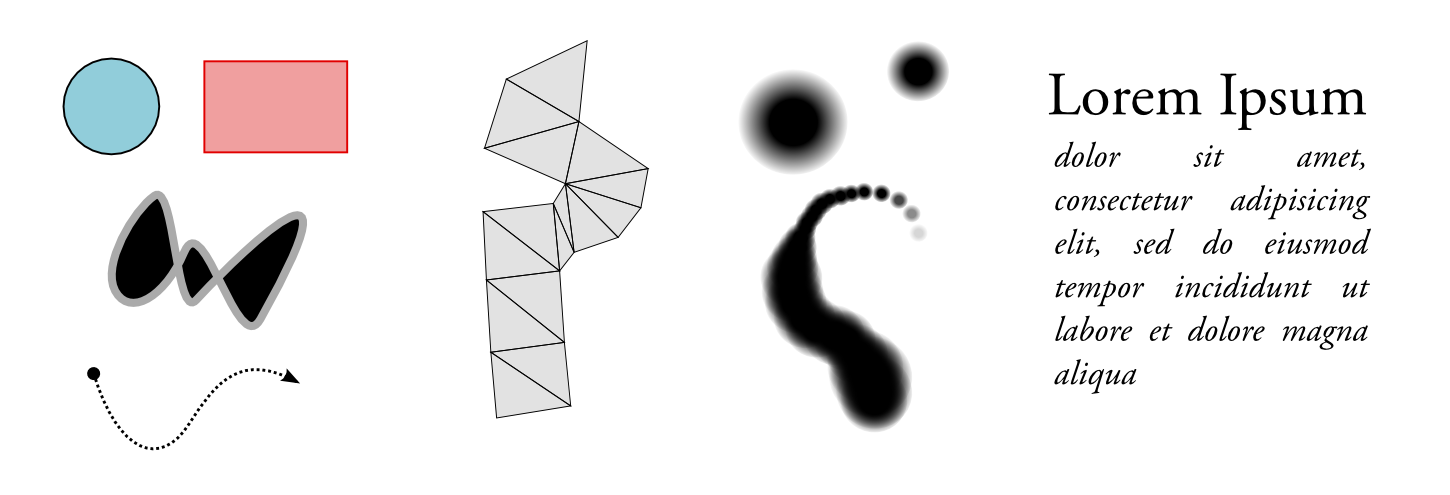
\includegraphics[width=\textwidth]{images/primitives}
					\caption{Examples de dessins de primitives}
					\label{fig:primitives}
				\end{figure}
			\subsubsection{Filtres}
				\index{Filtres}
				Un filtre est une opération qui modifie l'aspect de l'entièreté d'une image. Le temps de calcul d'un filtre varie
				énormément d'un filtre à l'autre. Les plus simples prennent quelques microsecondes et peuvent aisément être exécutés
				en temps réel. D'autres prennent plusieurs dixaines de minutes. Certains frameworks ne sauront intégrer que les filtres
				les plus rapides. 

				Les filtres peuvent être également partagés en deux catégories,\index{Filtres!colorimetriques} les filtres colorimétriques qui transforment
				la couleur d'un pixel sans se soucier de la couleur des pixels voisins, \index{Filtres!spatiaux} et les filtres spatiaux nécessitant 
				eux d'en connaître plusieurs. 
				\begin{figure}[h]
					\centering
					\subfloat[Image originale]{ \label{fig:lenna} 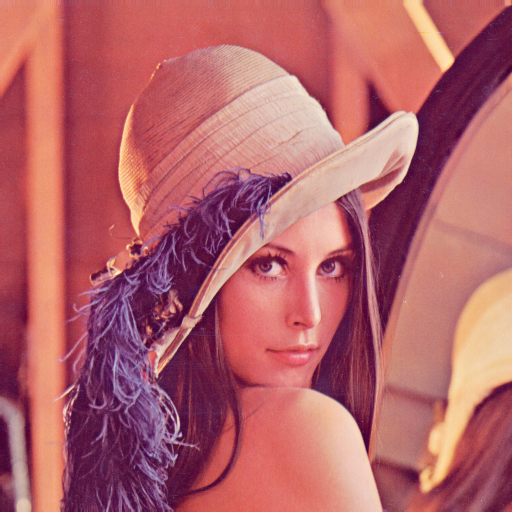
\includegraphics[width=0.3\textwidth]{images/Lenna} }
					\subfloat[Filtre colorimétrique]{ \label{fig:lenna} 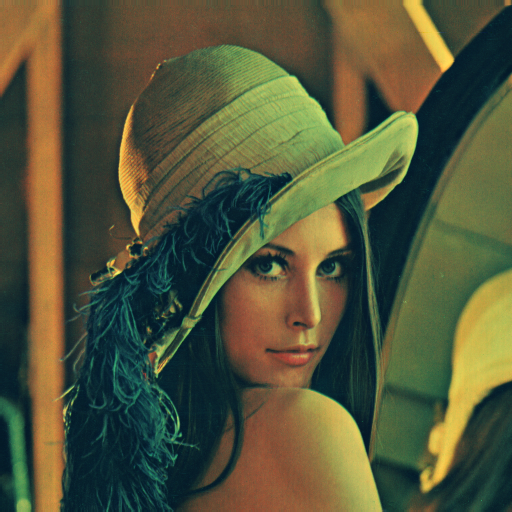
\includegraphics[width=0.3\textwidth]{images/Lenna-green} }
					\subfloat[Filtre spatial \emph{Sobel}]{ \label{fig:lenna} 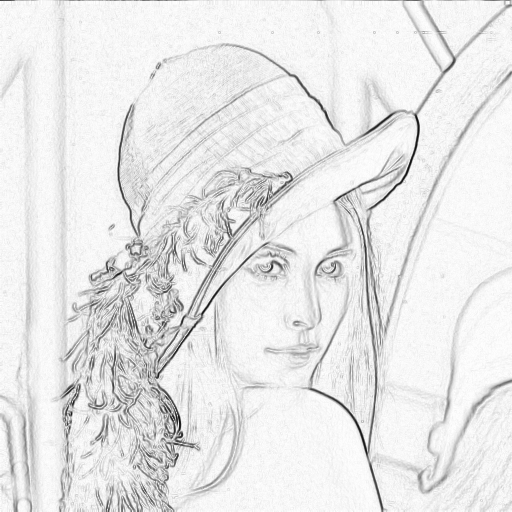
\includegraphics[width=0.3\textwidth]{images/Lenna-sobel} }
					\caption{Examples de filtres}
					\label{fig:filtres}
				\end{figure}
			\subsubsection{Transformations géométriques}
				Les transformations géométriques modifient la forme d'un objet constituant l'image; rotation, translation, 
				redimentionnement et perspective sont les applications les plus courantes. 
				
				Il y a deux approches pour implémenter les transformations
				géométriques: l'approche vectorielle consiste à modifier la description de l'image avant la rasterisation. L'approche
				bitmap consiste à modifier les pixels après leur rasterisation. Cette deuxième approche, nettement plus lente, permet
				cependant d'implémenter des transformations non linéaires, telle que les transformées polaires, la correction de distortion de 
				lentille, ou les déformations fluides. 
				
			\subsubsection{Fusion et modes de fusion}
				La fusion consiste à fusionner deux images en une. On utilise pour cela une fonction nommée \emph{mode de fusion}.
				Elle à la forme $f(p_A ,p_B ,\alpha)$, où $p_A$, $p_B$ sont deux pixels des images $A$,$B$ que l'on veut fusionner. 
				$\alpha$ représente un ou plusieurs paramètres additionnels qui peuvent	modifier l'effet de la fonction.

				Le \emph{mode de fusion} la plus courante est celui de mélange par opacité: $f(p_A, p_B, \alpha) = \alpha * p_A + (1-\alpha) * p_B$,  $\alpha \in [0,1]$ 
				représentant l'opacité de $B$, mais il en existe bien d'autres.

				On peut utiliser cette fonction pour fusionner deux images en une nouvelle : $ C = f(A,B,\alpha)$, ou pour intégrer une image dans
				une autre $A = f(A,B,\alpha)$

				Puisque chaque dessin de primitive consiste en la fusion de celle ci sur l'image de fond, la fusion est une opération centrale
				dans tout framework. Cependant beaucoup d'entre eux se limitent au seul mode de mélange par opacité.

				\begin{figure}[h]
					\centering
					\subfloat[Image A]{ \label{fig:A} 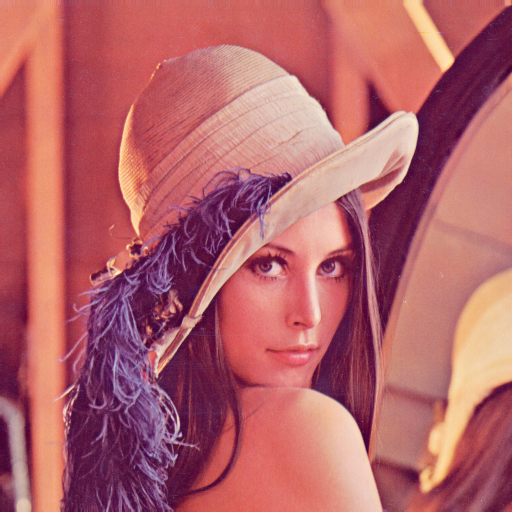
\includegraphics[width=0.25\textwidth]{images/Lenna} }
					\subfloat[Image B]{ \label{fig:B} 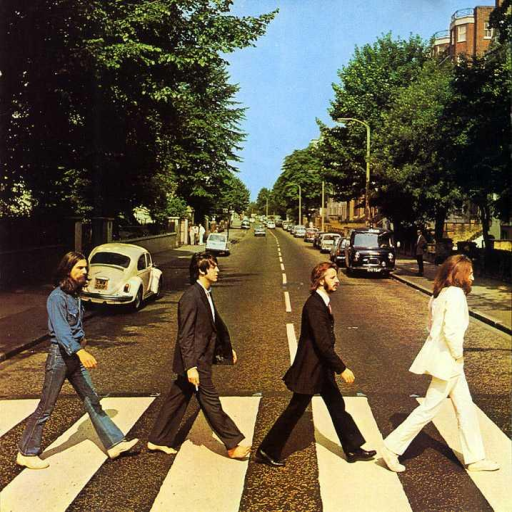
\includegraphics[width=0.25\textwidth]{images/abbey-road} }
					\subfloat[Blending de B sur A, par \emph{fusion de grain} ]{ \label{fig:ABfusion} 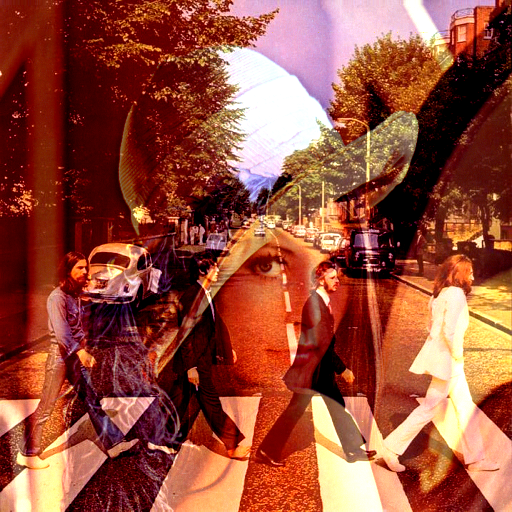
\includegraphics [width=0.25\textwidth]{images/abbey-road-lenna-fusion} }
					\subfloat[Blending de B sur A, par \emph{soustraction} ]{ \label{fig:ABsoustraction} 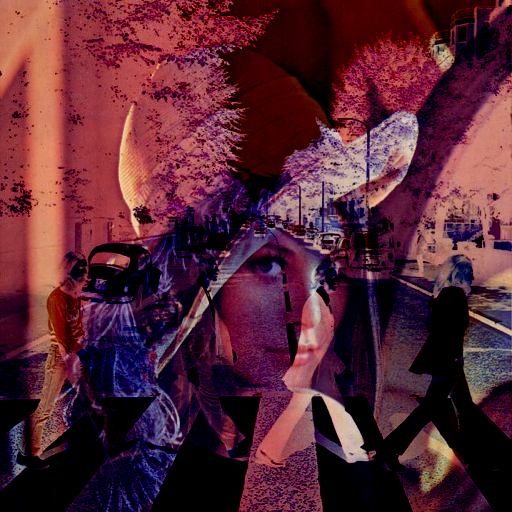
\includegraphics [width=0.25\textwidth]{images/abbey-road-lenna-substract} }
					\caption{Examples de blending}
					\label{fig:blending}
				\end{figure}

		\subsection{Modèles colorimétriques}
			La rasterisation d'une image permet de définir la couleur de chaque pixel. Or il existe de nombreuses manières de définir une même couleur.
			La manière la plus populaire est de définir la couleur comme un vecteur dans un espace colorimétrique. Chaque espace ayant sa propre utilité:
			\begin{description}
				\item[Le RGB] est l'espace utilisé par les écrans et projecteurs, ainsi que les capteur photographiques. Toute couleur doit donc être
				convertie en RGB avant d'être affichée. Il existe plusieurs espaces RGB définis par des couleurs primaires Rouges, Vertes et Bleues différentes.
				Le plus utilisé est le sRGB, qui est le standard d'affichage des écrans.
				\item[Le Yuv] est l'espace utilisé par les vidéos et par certains formats de fichier comme le JPEG.
				L'espace Yuv permet en effet une meilleure compression des données.
				\item[Le CIELab] est l'espace utilisé en retouche photo, il permet de manipuler les couleurs de manière conforme à la perception humaine.
				\item[Le HSL] est un espace qui permet de décrire les couleurs en composantes de teintes, de saturation et de luminosité, notions
				facilement compréhensibles et manipulables. Cet espace est utilisé pour certains filtres et pour l'édition des couleurs.
				\item[Le CMYK] est l'espace utilisé par les imprimantes jet d'encre, chaque imprimante ayant ses propres couleurs primaires. 
				Toute image doit donc être convertie dans le CMYK correspondant à l'imprimante avant d'être imprimée.
			\end{description}
			Il existe encore bien d'autres espaces colorimétriques spécifiques à des applications industrielles particulières. 

			Pour compliquer le tout, les espaces colorimétriques ne se superposent généralement pas. Ainsi des couleurs qui peuvent s'exprimer dans l'un n'existent pas
			dans l'autre. Un framework dédié à l'impression doit ainsi prendre garde de n'afficher en RGB que des couleurs disponibles dans le CMYK de l'imprimante.

			Une autre manière de décrire les couleurs est d'utiliser un nuancier contenant une liste de couleurs standardisées. Ce système est utilisé dans les images destinées à l'impression
			afin d'identifier des encres dont l'apparence ne peut être réduite à une simple couleur, comme les encres mattes, brillantes, métallisées,
			fluorescentes, etc. Dans ce cas chaque pixel possède une certaine quantité de chacune des  couleurs utilisées pour décrire l'image.

			\subsubsection{Quantisation}
			Les composantes d'un pixel peuvent aussi être quantifiées à différents degrés: 1bit pour les systèmes halftone; 8bit pour l'affichage 
			à l'écran,  les textures de jeux vidéos; 32 bit flottant permet d'avoir des valeurs de couleurs dépassant les capacité d'affichage
			d'un écran, ce qui est particulièrement intéressant pour l'édition non destructive d'image utilisée en photographie et en 
			effets spéciaux. La précision apportée par une telle profondeur est également indispensable pour le cinéma numérique.

			\subsubsection{Extensions de modèles colorimétriques}

			Enfin, il arrive qu'un pixel ne décrive plus une couleur mais une information quelconque de lá partie de l'objet qu'il représente.
			On rencontre ainsi la distance du pixel à l'observateur, la normale de la surface, un identifiant unique de l'objet, la vitesse de
			déplacement de l'objet, etc. Ces informations sont généralement fournies en plus des informations colorimétriques habituelles.

			Ce type d'information est typiquement fourni par la caméra ou généré par le moteur de rendu afin de faciliter l'intégration d'effets
			spéciaux à l'image. Le type d'information utilisés apparaissent et disparaissent avec les technologies, nécessitant une grande 
			flexibilité dans leur gestion. Les \emph{Éditeurs Nodaux} sont particulièrement adaptés à la gestion de ce type d'informations.
			
			\begin{figure}[h]
				\centering
				\subfloat[Couleurs vraies]{ \label{fig:render} 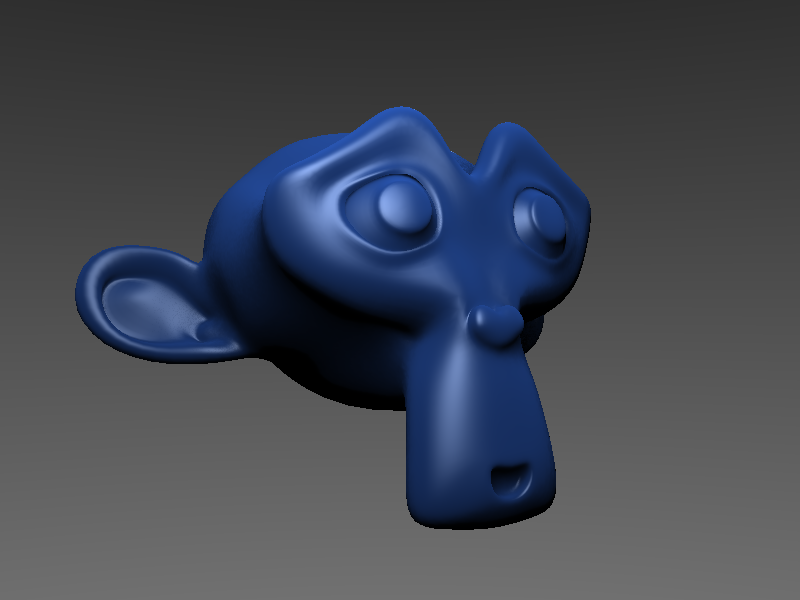
\includegraphics[width=0.25\textwidth]{images/render} }
				\subfloat[Format HSV en fausses couleurs]{ \label{fig:render-hsv} 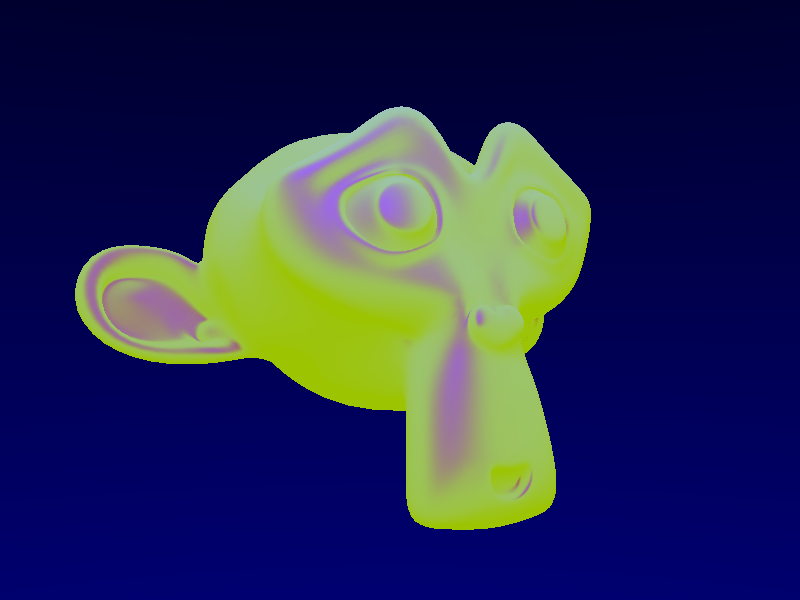
\includegraphics[width=0.25\textwidth]{images/render-hsv} }
				\subfloat[Vecteur normal de la surface]{ \label{fig:render-normal} 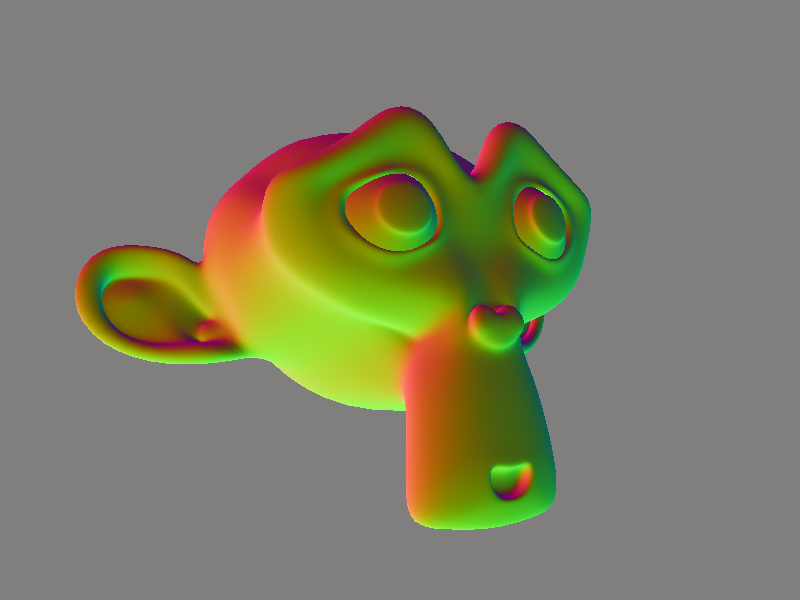
\includegraphics [width=0.25\textwidth]{images/render-normal} }
				\subfloat[Distance à l'observateur]{ \label{fig:render-depth} 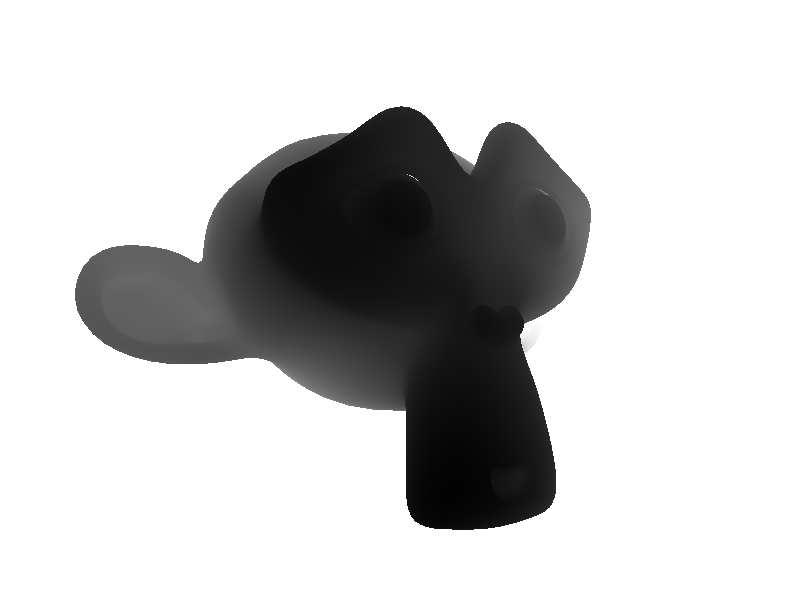
\includegraphics [width=0.25\textwidth]{images/render-depth} }
				\caption{Examples d'espaces colorimétriques et de métadonnées}
				\label{fig:color}
			\end{figure}

		\subsection{Undo / Redo}
			Un framework a souvent des mécanismes internes permettant une gestion efficace d'annulation et de répétiton des opérations.
		\subsection{Édition non destructive}
			L'édition non destructive consiste à pouvoir modifier les opérations après leur application sans perte de qualité de l'image.
		\subsection{Composition non linéaire}
			La composition non linéaire permet à une opération d'utiliser le résultat d'une opération autre que celle appliquée précedemment. Idéalement
			le résultat de cette opération ne doit pas être recalculé. Cette fonctionalité permet de combiner des effets simples afin d'obtenir des
			effets beaucoup plus complexes que ce qui est possible par composition linéaire, et permet souvent à l'utilisateur d'éviter de devoir 
			programmer ses propres effets. De nombreux logiciels présentent ainsi une interface nodale 
			comme alternative à la programmation de pixel-shaders.

		\subsection{Édition par pixel}
			Certains frameworks permettent d'éditer individuellement chaque pixel de l'image. 
		\subsection{Indépendance à la résolution}
			La description de l'image est indépendante de la résolution utilisée pour la rasterisation; Il n'y a pas de dégradation
			de la qualité de l'image quelque soit la résolution utilisée pour le rendu. L'édition par pixel et l'indpendance à la résolution
			sont deux fonctionalités mutuellement exclusives.
		\subsection{Images gigapixels}
			Les images gigapixels sont les images constituées de plus d'un milliard de pixel, qui peuvent être plus grandes que la mémoire
			vive disponible. Il ne faut pas confondre édition d'images gigapixel et indépendance à la résolution.
			Si l'indépendance à la résolution permettent de décrire des documents de tailles aussi grande
			que désirée et de les rasteriser en des images gigapixel,ils ne permettent pas de décrire ou d'éditer des images
			de plus d'un milliard de pixels indépendants. 

		\subsection{Traitement d'images multiples}
			Le traitement d'images multiples consiste à savoir appliquer facilement les mêmes opérations sur un large nombre d'images similaires, 
			comme par exemple les photos d'une séance de shooting, les frames d'une vidéo ou d'un moteur 3D.

	\section{Frameworks Bitmaps}
		\subsection{Schéma de représentation de l'image}
			\begin{figure}[h]
				\centering
				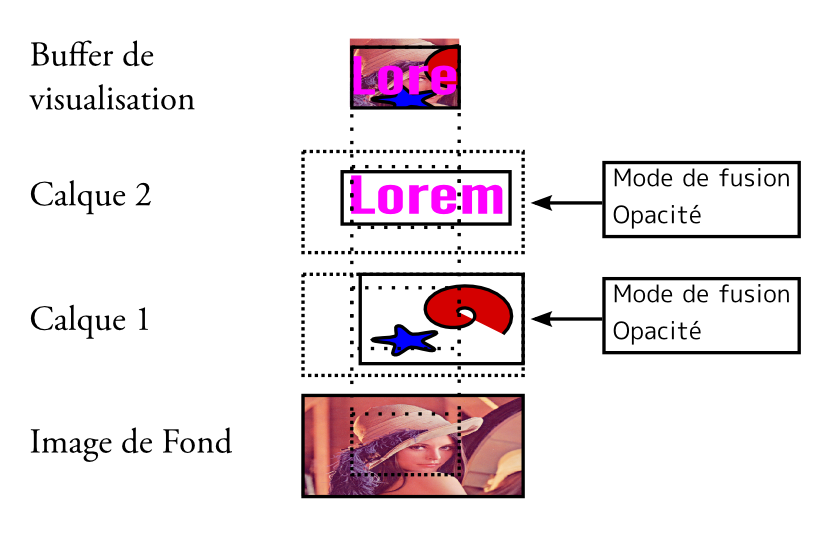
\includegraphics[width=0.6\textwidth]{images/calques}
				\caption{Représentation d'une image par calques}
				\label{fig:editbitmap}
			\end{figure}
			Dans un framework bitmap l'image est représentée directement sous sa forme rasterisée. 
			
			Une extension populaire est de décomposer l'image en une image de fond et une superposition de calques qui sont des bitmaps possèdant chacun leur propre
			dimension, position, un mode de fusion, et des paramètres d'opacité. Cette extension permet à l'utilisateur de pouvoir facilement modifier des zones
			spécifiques de l'image.

			Des frameworks extendent encore ce principent en décomposant les calques en sous calques, et ce de manière récursive. 

		\subsection{Algorithme de rasterisation}
			Dans un framework bitmap, chaque opération est directement rasterisée à la résolution native lors de son application. 
			
			Pour visualiser une région à une échelle différente de la résolution native, On utilise un buffer de visualisation de la taille
			de cette région dans lequel la région d'intérèt est mis à l'échelle voulue après chaque rasterisation.
			
			Lorsqu'un système de calques est utilisé, on rasterise d'abord directement l'opération sur le calque modifié. On place ensuite l'image
			de fond dans le buffer de visualisation. Chaque calque y est ensuite fusionné.			
			
			Comme la plupart des opérations ne modifie qu'une petite partie de l'image, on aimerait éviter de devoir fusionner l'intégralité
			des calques à chaque fois. Il y a deux approches pour cela: La première est de demander à chaque opération de spécifier la région
			qu'elle modifie. On ne modifie ensuite le buffer de visualisation que pour cette région. 

			La deuxième approche consiste à diviser l'image de fond et les calques en une grille de sous régions aux dimensions régulières appelées
			tiles. Lors de l'application de l'opération, celle ci ne modifiera que certains tiles. Seuls les tiles correspondants dans les calques
			et l'image de fond seront fusionnés dans le buffer de visualisation. Les tiles peuvent également être traités en parallèle sur une 
			machine multi-processeur.

			Les tiles ont d'autres intérèts que d'accélérer la rasterisation; En omettant les tiles des zones transparentes des calques ou réduit 
			l'espace mémoire qu'ils consomment. En outre, les tiles peuvent être migrés vers le disque dur lorsqu'il n'est plus possible de tous
			les stoquer en mémoire, ils sont ensuite récupérés lorsqu'ils sont utilisés. 
			
			Il n'est cependant pas toujours possible d'implémenter une opération pour qu'elle fonctionne tile par tile. Dans ces cas on devra placer
			les tiles dans un buffer temporaire et les récupérer après l'opération. 

		\subsection{Fonctionalités adaptées aux frameworks bitmaps}
			\subsubsection{Opérations de dessin}
				Étant donné qu'il n'est pas nécessaire de maintenir une liste de toutes les opérations appliquées sur l'image, les frameworks
				bitmaps sont particulièrement efficaces lorsqu'un très grand nombre de celles-ci sont utilisés ce qui est le cas pour les
				logiciels de peinture. 
			\subsubsection{Undo / Redo}
				L'undo/redo est implémenté en gardant une copie de la région/tiles modifiée par l'opération avant sa modification. 
				Il suffit ensuite de réutiliser ces copies pour obtenir la version sauvegardée. Garder les copies consomme beaucoup de mémoire,
				et une limite d'historique est nécessaire pour pallier à ce problème. En revanche, annuler ou refaire une opération ne demande
				pas de recalculer l'opération et est donc très rapide.
		\subsection{Fonctionalités inadaptées aux frameworks bitmaps}
			\subsubsection{Modèles colorimétriques et métadonnées}
				L'architecture des frameworks bitmaps limite sévèrement les possibilité de gestion de modèles colorimétriques et de métadonnées.
				En effet, comme chaque opération est rasterisée dans le calque dès son application, les opérations doivent nécéssairement 
				avoir le même modèle colorimétrique en entrée et en sortie. Elles doivent aussi comprendre le modèle colorimétrique et extensions du 
				calque, ce qui nécessite de devoir soit modifier les opérations à chaque ajout de nouveau type de modèles colorimétriques et d'extensions
				soit de passer par de couteuses transformations de modèles.

				Il exite une solution permettant d'améliorer la situation : Au lieu de placer tous les composants du pixel dans un même calque, on
				divise le calque en sous calques appelés canaux qui contiennent chacun un seul composant du pixel. Les opérations sont ensuite 
				codées pour prendre des canaux en entrée et en sortie. Il est maintenant possible d'ignorer les canaux inutiles, d'avoir des canaux
				de différentes précision, et de changer la signification d'un canal lors de l'application d'une opération. 

				Cette approche à pour inconvénient de ralentir nettement les opérations, puisqu'il faut désormais accéder des zones de 
				mémoire fort éloignées pour lire ou modifier un seul pixel. 

				En pratique les framework bitmap implémentent un nombre limité de modèles colorimétriques, et imposent
				le même modèle pour tous les calques d'une image. 
			\subsubsection{Images gigapixel}
				Il est théoriquement possible de gérer des images de taille plus grande que la mémoire disponible en utilisant les tiles à
				bon escient. Mais en pratique, chaque opération nécessite d'être appliquée intégralement sur l'image à résolution native, 
				ce qui est infaisable de manière interactive pour des opérations modifiant de grandes parties de l'image.
			\subsubsection{Édition non destructive}
				L'édition non destructive requiert de garder une liste de toutes les opérations effectuées sur l'image, afin de pouvoir
				modifier l'opération désirée, et de refaire celles qui doivent être réappliquées. 

				Il est cependant possible d'implémenter des opérations non destructives en tant que calques à part entière. 
				Si l'opération est un filtre spatial, il faudra pouvoir étendre le buffer de rasterisation pour que le filtre ait accès aux données
				nécessaires. Et s'il s'agit d'un filtre de transformation, la zone à modifier dans le buffer de visualisation devra elle aussi
				être modifiée au fur et à mesure des filtres. Tout cela étant fort compliqué à implémenter, sans garantie de performances, 
				les frameworks confinent généralement l'édition non destructive aux filtres colorimétriques et dessin de primitives.
		\subsection{Framework bitmaps, l'état de l'art}
			\begin{description}
				\item[Adobe Photoshop] Logiciel de peinture et retouche photo
				\item[Corel Painter] Logiciel de peinture
				\item[Artrage] Logiciel de peinture
				\item[Gimp $\leq$ 2.6] Logiciel de peinture et retouche photo open source
				\item[Krita] Logiciel de peinture et retouche photo open source
				\item[Blender3d] Utilisé pour la peinture de texture, Logiciel d'animation 3D.
				\item[psd] Format d'image de photoshop
				\item[xcf] Format d'image de Gimp.
			\end{description}

	\section{Frameworks Nodaux}
		\subsection{Schéma de représentation de l'image}
			\begin{figure}[h]
				\centering
				\subfloat[En rouge les noeuds d'entrée, en orange les noeuds d'opération, en vert les noeuds de visualisation]{ \label{fig:render} 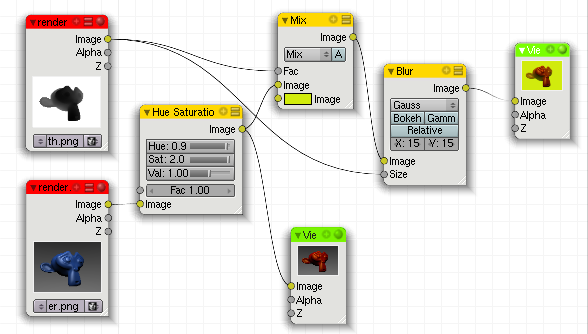
\includegraphics[width=0.6\textwidth]{images/nodes} }
				\subfloat[Image calculée par le graphe (a)]{ \label{fig:render-hsv} 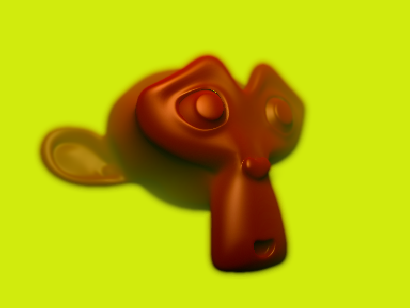
\includegraphics[width=0.4\textwidth]{images/nodes-out} }
				\caption{Example d'édition nodale d'images telle qu'implémenté par \emph{Blender 2.49}}
				\label{fig:editnodal}
			\end{figure}
			Les frameworks nodaux représentent l'image par un graphe composé de trois types de noeuds.
			\begin{itemize}
				\item Les noeuds d'entrée servent à spécifier les images à modifier et ne proposent que des sorties.
				\item Les noeuds d'opération prennent en entrée des images et/ou des canaux et/ou des paramètres,
				et proposent en sortie le résultat des images et/ou des canaux et/ou des valeurs, résultats de
				l'opération sur les entrées.
				\item Les noeuds de visualisation n'ont qu'une entrée et servent à visualiser sa valeur, que ce soit un paramètre,
				un canal ou une image. Dans le cas de canaux ou d'images, le noeud peut également spécifier une sous région
				de l'image et une échelle.
			\end{itemize}
			Le graphe est acyclique et dirigé; chaque arrète va de la sortie d'un noeud à une entrée d'un autre. Il peut
			y avoir plusieurs arrètes partant d'une sortie, mais une seule arrivant à chaque entrée. 
		
		\subsection{Algorithme de rasterisation}
			Pour obtenir la sortie d'un noeud, il faut premièrement obtenir toutes ses entrées, et appliquer l'opération du
			noeud s'il y en a une. On appliquera donc ce principe de manière récursive en partant d'un noeud de visualisation,
			la récursion s'arrètant au noeuds d'entrée.

			Si le noeud de visualisation spécifie une sous-région de l'image, l'algorithme fonctionne de manière identique, à
			ceci près que les opérations pouvant transformer géométriquement l'image, la région en entrée ne sera pas la même que
			la sortie. Il faut donc que le noeud soit capable d'inverser la transformation qu'il effectue afin de demander la bonne
			région à ses parents. 

			Si le noeud de visualisation spécifie une échelle, les images fournies par les noeuds d'entrée sont mises à l'échelle avant
			leur sortie, de même que les paramètres métriques des opérations. 

			Comme une sortie peut être connectée à plusieurs entrées, une même opération peut être calculée plusieurs fois. Pour éviter
			cela, chaque noeud peut disposer d'une cache dans laquelle il place le résultat de ses sorties. 

			Les images utilisées peuvent également utiliser une représentation par tiles afin de bénéficier des avantages de gestion d'images
			volumineuses.

		\subsection{Fonctionalités adaptées aux frameworks nodaux}
			\subsubsection{Édition non destructive}
				C'est un des gros points forts des frameworks nodaux. On peut facilement modifier les paramètres et la topologie du graphe
				et visualiser le résultat.
			\subsubsection{Composition non linéaire}
				La composition non linéaire découle de l'architecture en graphe des frameworks nodaux. Les frameworks nodaux sont d'ailleurs
				les seuls frameworks permettant une réelle édition non linéaire. 
			\subsubsection{Modèle colorimétrique}
				Un framework nodal offre une liberté totale à l'utilisateur en ce qui concerne les modèles colorimétriques. Si un noeud sort
				une image en RGB, et qu'une opération attend du YUV, il peut les connecter ensemble. Le canal R sera interprété comme Y, le G comme
				U et le B comme V. S'il désire garder l'interprétation colorimétrique du RGB, il devra utiliser un noeud qui convertit le RGB en YUV.

				Intégrer un nouveau modèle colorimétrique se limite donc à créer des noeuds de conversions et les noeuds d'opération qui peuvent
				tirer bénéfice de ce nouveau modèle.

				L'édition nodale est cependant incapable de gérer les tons directs.
			
				
			\subsubsection{Images gigapixel}
				La complexité en temps et en mémoire de la rasterisation d'une image ne dépend tout au long du graphe que de la taille de
				la région du noeud de visualisation. Une borne supérieure de la taille de ces région est la résolution des écrans qui ne
				dépasse pas les quelques mégapixels. Il reste l'opération d'échelle à effectuer au niveau des région d'entrée. Si on
				dispose de mipmaps de ces images, alors il est possible d'effectuer des opérations sur images gigapixels de manière efficace.
			\subsubsection{Traitement d'images multiples}
				Le même graphe peut très facilement s'appliquer sur un grand nombre d'images de manière automatique, ce qui rend ces frameworks
				particulièrement adaptés au traitement vidéo.
				
		\subsection{Fonctionalités inadaptées aux frameworks nodaux}
			\subsubsection{Undo/Redo}
				On peut s'attendre d'un framework permettant l'édition non destructive d'exceller dans l'undo/redo. Cependant, il n'est pas
				facile de gérer les changements de paramètres des noeuds et de la topologie du graphe tout en maintenant des caches cohérentes.
				C'est pourquoi les graphes nécessitent souvent d'être rasterisés à nouveau ce qui peut prendre du temps lorsque celui ci contient
				des filtres complexes. 
			\subsubsection{Opération de dessin de primitves}
				Il est tout à fait possible de créer des noeuds dessinant des primitives, et de les connecter entre eux pour avoir une topologie
				semblant correspondre aux frameworks bitmaps ou vectoriels. 

				Un premier problème est que les frameworks nodaux appliquent les opérations de transformations sur les pixels constituant la primitive et non sur les paramètres la définissant.
				Par exemple, il sera impossible de récupérer l'apparence exacte de la primitive après une transformation d'échelle 
				la réduisant à un seul pixel. Cet exemple extrême démontre comment à chaque transformation successive, la primitive est peu à peu
				dégradée. Un framework vectoriel n'a pas ce genre de problèmes.
				
				Ensuite, un framework nodal est une entité complexe, et il devient impossible à l'utilisateur de gérer un graphe contenant 
				autant de noeuds que nécessiterait la réalisation d'une peinture. Sans parler de la consommation en mémoire du graphe, 
				et de la surcharge de calcul qu'entraine le parcours de celui-ci.

				On ne peut pas non plus se permettre de devoir recalculer toutes les opérations de dessin à chaque Undo/Redo, à chaque édition
				non destructive et à chaque nouvelle visualisation.

				Les frameworks nodaux font donc souvent le choix d'ignorer totalement les opérations de dessin. Celles-ci sont alors effectuées
				sur les images avant leur entrée dans le graphe, et doivent être gérées par un autre framework tel qu'un framework vectoriel ou bitmap.

				Certains frameworks nodaux (GEGL) choisissent de proposer des noeuds qui regroupent une séquence d'opération de dessin en une seule.
				Ces noeuds sont donc obligés de gérer par des mécanismes interne l'undo/redo. De tels noeuds fonctionnant comme des frameworks bitmaps
				ils ne peuvent pas gérer des opérations de dessin de trop grande taille. 
				
				Ces frameworks permettent donc de peindre sur des images gigapixel, mais chaque trait de peinture doit rester de taille mégapixel,
				ce qui limite l'utilité de cette fonctionalité dans le cadre d'édition d'images gigapixel.


			\subsubsection{Édition par pixel}
				L'édition par pixel est problématique pour les mêmes raisons qui rendent problématique le dessin de primitives.
		\subsection{Framework nodaux, l'état de l'art}
			\begin{description}
				\item[The Foundry Nuke]Logiciel de composition et post processing vidéo
				\item[Blender3D]Utilisé pour la composition et le post processing vidéo, logiciel d'animation 3D open source.
				\item[GEGL]Framework nodal open source utilisé par Gimp $\geq$ 2.7 et le logiciel d'acquisition numérique Gnome Scan.
				\item[OpenRaster]Format d'image public permettant de sauvegarder des graphes d'opérations et compatible avec GEGL.
			\end{description}

	\section{Framework vectoriel}
		\subsection{Schéma de représentation de l'image}
			\begin{figure}[h]
				\centering
				\subfloat[l'image]{ \label{fig:render} 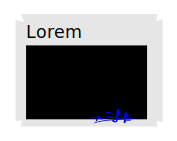
\includegraphics[width=0.33\textwidth]{images/scenegraph-img} }
				\subfloat[Le graphe de scène]{ \label{fig:render-hsv} 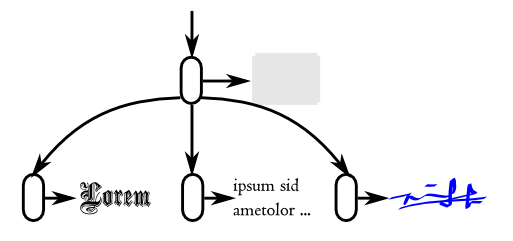
\includegraphics[width=0.66\textwidth]{images/scenegraph-graph} }
				\caption{Représentation d'une image par graphe de scène}
				\label{fig:editnodal}
			\end{figure}
			L'image est décrite par un emsemble de primitives géométriques. Ces primitives sont organisées dans un graphe de scène. Dans un 
			graphe de scène, chaque noeud représente une transformation géométrique et une primitive. La transformation géométrique détermine
			la position, l'échelle, et la rotation de la primitive et de ses enfants. La primitive est elle décrite par son type et les paramètres
			qui déterminent sa forme et son apparence.

			Le graphe de scène est acyclique. chaque noeud peut avoir plusieurs enfants et sauf exception un seul parent. 

			L'ordre des enfants d'un noeud est important puisqu'ils déterminent l'ordre dans lequel ils seront dessinés. Ainsi les derniers
			enfants d'un noeuds seront dessinés au dessus des premiers. 

			Chaque framework a sa propre liste de primitives géométriques, mais tous disposent au moins de points, lignes, ploygones, ellipses,
			texte, et courbes de bézier.

		\subsection{Algorithme de rasterisation}
			L'utilisateur commence d'abord par choisir la région qu'il veut rasteriser et à quelle résolution. Le framework crée ensuite un bitmap
			de cette taille et résolution de la couleur de fond de l'image.

			Pour dessiner un noeud du graphe, on applique sa transformation aux paramètres de sa primitive. On dessine ensuite cette 
			primitive sur le bitmap. On Dessine ensuite chaque noeud enfant dans l'ordre en leur appliquant la transformation de ce noeud.

			Cette opération est effectuée de manière récursive en partant du noeud racine de l'image.

			Afin d'éviter de dessiner les primitives qui se trouvent en dehors de la région à rasteriser, on associe à chaque noeud une boite
			qui englobe sa primitive ainsi que celles de tous ses enfants. Si la boite est en dehors de la région, on peut ignorer ce noeud et
			leurs enfants. 

			Afin d'exploiter l'accélération matérielle, la plupart des frameworks ne dessinent pas directement les primitives, mais les 
			convertissent en triangles qui sont ensuite dessinés à l'aide du matériel. Cette approche peut également s'avérer bénéfique 
			sans accélération matérielle car le dessin de triangle est souvent beaucoup plus rapide qu'un dessin analytique de la primitive,
			de plus les détails trop petits pour être vus peuvent être détectés lors de la transformation de la primitive en triangles.

		\subsection{Fonctionalités adaptées aux frameworks vectoriels}
			\subsubsection{Édition non destructive}
				La description de la scène étant gardée en mémoire, il est facile de la modifier et d'obtenir ensuite une nouvelle visualisation.
				L'algorithme de rasterisation ne disposant généralement pas de cache, l'intégralité de la région à visualiser doit être recalculée à chaque 
				modification de l'image. Cela n'est pas un problème tant que la taille du graphe de scène reste raisonnable.
			\subsubsection{Undo / Redo}
				L'undo/redo est simple à implémenter et aussi efficace que l'édition non destructive. 
			\subsubsection{Opérations de dessin de primitives}
				Les frameworks vectoriels sont très pratiques pour éditer un dessin constitué de primitives géométriques. Cependant, la région de
				visualisation doit être rasterisée à chaque changement d'échelle ou à chaque déplacement de celle-ci. Si le nombre de primitives
				constituant le dessin est trop grand, cela ne peut plus se faire de manière interactive.
				
				Les frameworks vectoriels sont donc généralement utilisés pour les documents textuels, les cartes, les graphes, ou les dessins abstraits
				qui peuvent être décrits par un petit nombre de primitives complexes. A contrario, les images peintes utilisent 
				un trop grand nombre de primitives pour que de tels frameworks soient efficaces. 
		\subsection{Fonctionalités inadaptées aux frameworks vectoriels}
			\subsubsection{Filtres}
				En associant les filtres aux noeuds on s'attend à ce que le filtre ne s'applique
				qu'à ce noeud et à ses enfants. Ceci nécessite de faire une rasterisation de ces noeuds dans un buffer séparé afin d'y appliquer le
				filtre, puis de réintégrer ce buffer dans le buffer en cours. Et ce de manière récursive selon qu'il y ait des filtres dans les
				noeuds enfants. 
				Tout cela ralentit nettement la rasterisation, d'autant que le rendu dans de multiples buffer ne fait pas bon ménage avec 
				l'accélération matérielle. Les frameworks proposent parfois de tels filtres, mais les performances suivent rarement.
				
				Le format vectoriel SVG propose des sémantiques de filtres plus complexes. Le fait qu'aucun framework ne les implémente correctement
				atteste de la difficulté de cette entreprise. 
			\subsubsection{Composition non linéaire}
				La structure arborescente du scene graphe ne permet pas de décrire des compositions non linéaires.
			\subsubsection{Édition par pixel}
				Éditer un pixel requiert de créer une primitive couvrant uniquement ce pixel. Si cela est possible, cela crée rapidement une trop
				grande quantité de noeuds au fur et a mesure que chaque pixel est modifié. De plus, une telle description pose de gros problèmes
				d'anti-aliasing pour les résolutions non natives. 
			\subsubsection{Images gigapixel}
				Les frameworks vectoriels décrivant l'image de manière analytique peuvent gérer des images de toutes tailles et résolutions. De 
				plus la description vectorielle utilise beaucoup moins de mémoire. Ces frameworks sont donc pour l'instant la solution de choix
				pour décrire des documents de grande taille. Cependant il ne s'agit pas là à proprement parler d'images gigapixel.  
			\subsubsection{Modèles colorimétriques}
				Tant la description de l'image que l'algorithme de rasterisation sont peu adaptés au support de multiples modèles 
				colorimétriques, à une exception près, le modèle par nuancier. Dans ce cas chaque primitive est associée à une couleur du nuancier,
				et à une opacité. L'image peut ainsi être envoyée sous forme vectorielle à l'imprimante qui va imprimer les primitives une à une
				en respectant la structure du graphe de scène. L'image peut également être rasterisée pour obtenir pour chaque pixel la proportion
				des encres à utiliser. 
		\subsection{Framework Vectoriels, l'état de l'art}
			\begin{description}
				\item[Adobe Illustrator]Logiciel d'édition graphique vectorielle. 
				\item[Corel Draw]Logiciel d'édition graphique vectorielle.
				\item[Adobe Flash]Logiciel d'animation 2D
				\item[Inkscape]Logiciel open source d'édition graphique vectorielle.
				\item[libart]Librairie open source de rendu et d'édition graphique vectorielle, utilisée par Gnome Canvas, Inkscape.
				\item[Cairo]Librairie open source de rendu et d'édition graphique vectorielle, utilisée par Mozilla Firefox, Webkit, Moonlight,
				FontForge, Poppler, Gtk+
				\item[ai]Format d'image vectorielles.
				\item[svg]Format public d'images vectorielles.
				\item[ps]Format et langage de programation public décrivant des images vectorielles, obsolète à de nombreux égards mais toujours utilisé pour l'impression de documents.  
			\end{description}

	\section{Mégatexturing ou Sparse Virtual Textures}
		Les scènes 3D interactives sont de plus en plus grandes et détaillées. Or les détails sont limités par la taille des textures que l'on peut y
		appliqué, qui sont elle même limitées par l'espace mémoire disponible sur la carte graphique. On était donc condamné jusqu'il y a peu à utiliser
		une des trois techniques suivantes, ou de les combiner : 
		\begin{itemize}
			\item Une grande texture basse résolution
			\item Une petite texture haute résolution qui se répète sur les surfaces
			\item Des textures vectorielles.
		\end{itemize}
		Aucune de ces techniques ne peuvent texturer un large environnement de manière convaincante. 

		Le Megatexturing, appelé aussi Sparse Virtual Texture est donc une technique d'affichage de textures plus qu'un framework à part entière. Le but de 
		cette technique est de permettre l'affichage et l'édition d'images gigapixel en tant que textures de scènes 3D interactives. Une image gigapixel
		étant suffisamment grande  pour couvrir l'intégralité de l'environnement à haute résolution.

		\subsection{Schéma de représentation de l'image}
			\begin{figure}[h]
				\centering
				\subfloat[La pyramide de tile représentant l'image complète]{ \label{fig:render} 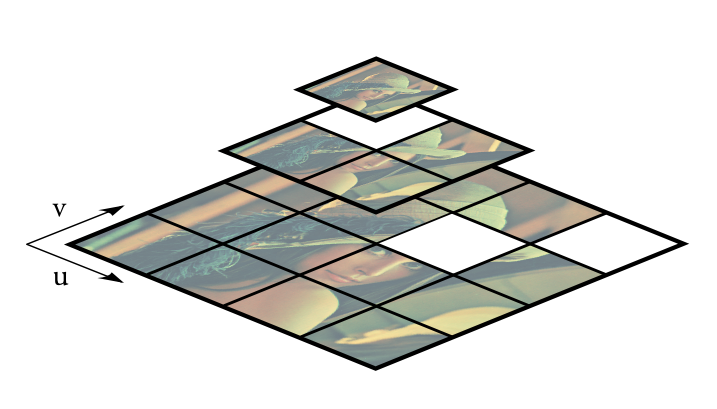
\includegraphics[width=0.6\textwidth]{images/megatextures-pyramid} }
				\subfloat[La texture virtuelle, composée de tiles de la pyramide]{ \label{fig:render-hsv} 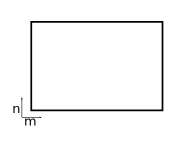
\includegraphics[width=0.4\textwidth]{images/megatextures-virtual} }
				\caption{Mégatexture}
				\label{fig:editmegatex}
			\end{figure}
		L'image est représentée par deux structures différentes, l'une se trouvant sur le disque et l'autre en mémoire.
		Celle qui se trouve sur le disque est la plus volumineuse des deux. Elle est composée d'une pyramide creuse de tiles. 

		Cette structure consiste en l'image gigapixel complète, divisée en tiles, les régions vides ou facultatives de l'image étant représentées par une absence
		de tiles, afin d'économiser de la mémoire. La structure contient aussi tous les mipmaps de cette image sous forme de tiles de dimensions identiques.

		En mémoire se trouve une texture, appellée \emph{texture virtuelle} qui a la taille maximum supportée par le matériel d'accélération, 
		ce qui est beaucoup moins que l'image originale. Cette texture est composée de tiles se trouvant dans la pyramide.
		
		\subsubsection{Affichage de l'image}
			Pour afficher une texture sur un maillage 3D, on assigne à chaque vertice  du maillage une coordonnée $u,v$ correspondant à un pixel de cette texture.
			de la texture. Comme nous désirons afficher la texture gigapixel, ces coordonnées correspondent aux pixels de cette texture.
			Celle-ci est cependant trop grande pour pouvoir être utilisée telle quelle.
			
			Pour résoudre ce problème on place les tiles qui nous intéressent dans une texture virtuelle qui est suffisemment petite pour pouvoir
			être utilisée pour l'affichage. Un \emph{pixel shader} est ensuite utilisé pour traduire lors de l'affichage les coordonnées $u,v$ de la
			texture gigapixel en les coordonnées $m,n$ de la texture virtuelle. 

			Pour déterminer quels tiles nous intéressent, on s'aide d'un premier rendu dans lequel on examine quelles régions de la texture gigapixel
			sont affichées, et à quelle résolution. On sélectionne ensuite les tiles qui couvrent cette zone avec la résolution la plus proche de celle
			affichée. Comme la résolution de l'écran est plus petite que celle de la taille de la texture virtuelle, on disposera toujours d'une place
			suffisante pour couvrir la quantité de texture affichée.

			Récupérer les tiles sur le disque implique un délai non négligeable. Le megatexturing incorpore des techniques permettant de pallier à
			ce problème qui sortent du cadre de cette présentation.

		\subsubsection{Édition de l'image}
			Pour générer et éditer l'image gigapixel, on utilise la technique précédente pour l'affichage, et on utilise les techniques de framework 
			bitmap pour appliquer les opérations; Celles-ci sont directement rasterisées dans la pyramide de tiles.
		\subsubsection{État de l'art du MegaTexturing}
			Le Megatexturing à été développé par John Carmack d'id Software pour le moteur de jeu idTech4 et idTech5. Cette technique est utilisé
			par les jeux utilisant ces moteurs. D'autres moteurs tels que Torque ont réimplémenté cette technique.

	\section{Comparaison des différents framework}

	\begin{table*}
		\label{comparaison}
		\begin{tabular*}{\textwidth}{@{\extracolsep{\fill}} | l || c | c | c | c |}
			\hline
			Fonctionalité	 		& Bitmap 		& Nodal 		& Vectoriel 		& Himalaya 	\\
			\hline \hline	                                                                                                          
			Dessin de primitives	   	& $\medbullet$		& $\ominus$		& $\medbullet$	 	& $\medbullet$	\\
			Peinture		   	& $\medbullet$		& $\ocircle$		& $\ominus$		& $\medbullet$	\\
			Filtres	colorimétriques	   	& $\medbullet$		& $\medbullet$		& $\ominus$		& $\medbullet$	\\
			Filtres	spatiaux	   	& $\medbullet$		& $\medbullet$		& $\ominus$		& $\ocircle$	\\
			Transformations vectorielles   	& $\ocircle$		& $\ocircle$		& $\medbullet$	 	& $\ocircle$	\\
			Transformations bitmap   	& $\medbullet$		& $\medbullet$		& $\ominus$	 	& $\ominus$	\\
			Modes de fusion		   	& $\medbullet$		& $\medbullet$		& $\medbullet$	 	& $\medbullet$	\\
			Modèles colorimétriques	   	& $\ominus$		& $\medbullet$		& $\ominus$	 	& $\medbullet$	\\
			Ton direct		   	& $\ominus$		& $\ocircle$		& $\medbullet$	 	& $\ocircle$	\\
			Modèles étendus		   	& $\ocircle$		& $\medbullet$		& $\ocircle$	 	& $\ominus$	\\
			Undo/Redo		   	& $\medbullet$		& $\ominus$		& $\medbullet$	 	& $\medbullet$	\\
			Édition non destructive	   	& $\ocircle$		& $\medbullet$		& $\medbullet$	 	& $\medbullet$	\\
			Composition non linéaire	& $\ocircle$		& $\medbullet$		& $\ocircle$	 	& $\medbullet$	\\
			Édition par pixel		& $\medbullet$		& $\ocircle$		& $\ocircle$	 	& $\ominus$	\\
			Indépendance à la résolution	& $\ocircle$		& $\ominus$		& $\medbullet$	 	& $\ocircle$	\\
			Images Gigapixel		& $\ocircle$		& $\medbullet$		& $\medbullet$	 	& $\medbullet$	\\
			Traitement d'images multiples	& $\ominus$		& $\medbullet$		& $\ocircle$	 	& $\ominus$	\\
			\hline
			\multicolumn{5}{|l|}{ \tiny $\medbullet$ : Fonctionalité adaptée au framework.} \\
			\multicolumn{5}{|l|}{ \tiny $\ominus$ : Fonctionalité implémentable dans le framework, mais de manière limitée ou peu performante.} \\ 
			\multicolumn{5}{|l|}{ \tiny $\ocircle$ : Fonctionalité inadaptée au framework.}	\\
			\hline
		\end{tabular*}
		\caption{Grille de comparaison des fonctionalités. }
	\end{table*}

	Le tableau~\ref{comparaison}, (page~\pageref{comparaison}) permet d'avoir une vision globale des fonctionalités supportées par les différents 
	types de framework. On remarque que les frameworks proposent des fonctionalités très différentes, ce qui explique pourquoi chaque 
	domaine d'application tend à préférer un framework en particulier.

	Ce tableau permet aussi de comparer les frameworks existants aux fonctionalités adaptées au framework Himalaya qui est présenté dans ce mémoire. Cette
	comparaison reste en partie théorique puisque toutes ces fonctionalités n'ont pas été implémentées et soumises à des tests utilisateurs. 
	
	Néanmoins ce framework propose une combinaison intéressante de fonctionalité en combinant Peinture, Dessin de primitives, Édition non destructive, 
	Composition non linéaire et Images gigapixel. Non repris dans ce tableau est la possibilité -- encore théorique -- de pouvoir utiliser la technique
	de megatexture en combinaison avec \emph{Himalaya} afin de permettre l'edition non destructive des textures d'une scène 3D temps réel.

	La suite de ce mémoire se concentrera sur la présentation de l'architecture et des fonctionalités de base du framework Himalaya, pour se concentrer
	ensuite sur l'implémentation et l'évaluation par test utilisateurs des fonctionalités de peinture et d'édition d'images gigapixel, combinaison de
	fonctionalité n'étant proposée par aucun des frameworks existants.

\chapter{Framework Himalaya (20 pages) }
	Himalaya est un framework d'édition d'image s'inspirant des frameworks nodaux et de la technique de megatextures. Il fut conçu par moi même avant la
	réalisation de ce mémoire dans le but de créer un logiciel de peinture permettant l'édition non destructive, la composition non linéaire, et d'être
	compatible avec la technique de mégatexture afin de pouvoir être utilisé dans le jeu vidéo. 


	\section{Structures de données}
		\subsection{Les Tiles}
		Comme dans bien d'autres framework, les images d'himalaya sont divisés en grilles de tiles. Un tile est donc un bitmap rectangulaire correspondant
		à une petite région de l'image. Himalaya fait un plus grand usage des tiles que d'autres frameworks puisque toute opération prend des tiles
		en entrée et en sortie. Un tile représente donc la plus petite unité de traitement, et un intérèt particulier doit être apporté à sa conception.

		\subsubsection{Structure du tile}
			Il y a trois caractéristiques importantes à prendre en compte lorsque l'on conçoit un tile:
			\begin{description}
				\item[Sa taille en mémoire]Un premier intérèt des tiles est qu'ils sont une unité de mémoire pouvant être suffisemment petite
				pour tenir intégralement dans les caches du processeur et ainsi éviter des accès cache invalides fort coûteux en temps de calcul.
				Les processeurs de différent modèles ont différentes taille de cache et différentes manières de les gérer. Plus le tile est petit,
				plus il sera rapide de les traiter sur une grande gamme de processeurs.
				
				Cependant, si le tile est trop petit, les gains réalisés par sa taille sont perdu par la surcharge de travail que doit faire le
				framework pour gérer ces tiles. 

				En outre, si tous les tiles ont la même taille en mémoire, on réduit les risques de fragmentation, et on peut faire des
				allocateurs optimisés qui allouent les tiles de manière contigue et réutilisent les tiles libérés.

				\item[Sa taille en pixel] Si tous les pixels ont la même taille en pixel, alors les images de dimensions égales seront
				toujours divisées en tiles de la même manière, ce qui rend plus simples beaucoup d'algorithmes du framework.
				la programmation des opérations en sera également facilitée. 

				Cependant, un framework moderne doit prendre en compte la gestion de modèles colorimétriques, et niveaux de quantification
				différents. La représentation d'un pixel peut donc avoir des empreintes mémoire différentes, il faudra donc choisir entre
				avoir des tiles de même taille pixel, ou des tiles de même taille mémoire.

			\begin{figure}[h]
				\centering
				\subfloat[Un tile normal]{ \label{fig:render} 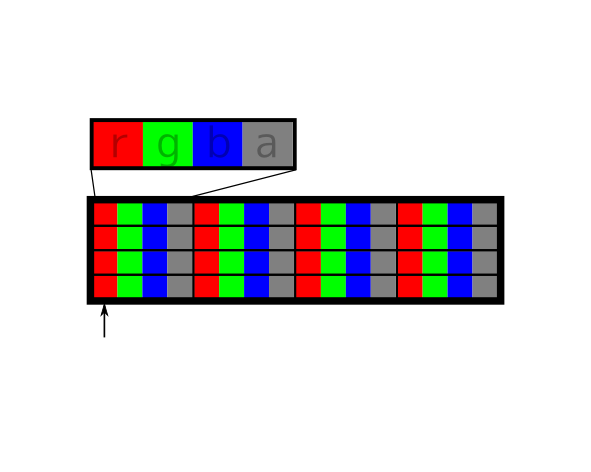
\includegraphics[width=0.5\textwidth]{images/tile-a} }
				\subfloat[Un tile aux canaux séparés]{ \label{fig:render-hsv} 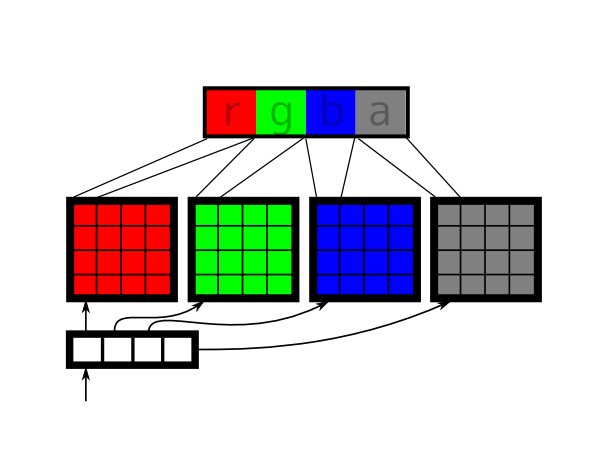
\includegraphics[width=0.5\textwidth]{images/tile-b} }
				\caption{Deux structures de tiles}
				\label{fig:tilestruct}
			\end{figure}
				\item[La répartition des pixels dans le tile] La manière commune de représenter un pixel au sein d'un bitmap est d'avoir
				toutes ses composantes placées dans des emplacement contigus. Une autre manière est de placer chaque composante dans un
				bitmap séparé. Un tile étant alors constitué de plusieurs bitmaps. L'intéret de cette technique est que les tiles de même
				quantisation ont la même taille en pixel, et les bitmaps les constituant la même taille en mémoire. Un autre intérèt est
				qu'il est maintenant beaucoup plus facile de programmer des opérations qui peuvent gérer un nombre quelconque de composantes
				par pixel.

				Cependant, cela implique que l'accès à un pixel nécessite autant d'accès mémoires que de composantes, ce qui ralentit 
				l'exécution du programme. 
			\end{description}

		\subsubsection{Comparaison des tiles}
			Le tableau TODO représente le résultat d'expériences qui résument les concepts précedemment exposés. Dans ce tableau, deux opérations
			sont testées : \emph{colorfill} consiste à remplir une image de $8192^2$ pixels \emph{RGBA} 8bits/composante d'une couleur unie. \emph{blend} consiste 
			en fusionner deux images de $8192^2$ pixels \emph{RGBA} 8 bits/composante par opacité. Ces deux opérations 
			sont utilisées très couramment pour la réalisation de peintures. 

			Ces opérations sont appliquées selon des schémas différents: \emph{colorfill\_full} remplit tous les tiles de l'image, alors que \emph{colorfill\_single}
			remplit un tile choisit au hasard autant de fois qu'il y a de tiles dans l'image. Le même nombre de pixels est donc traité dans les deux tests,
			mais le second devra accéder régulièrement à de nouvelles zones mémoire.

			Même chose pour les operations \emph{blend} : \emph{blend\_full} fusionne les tiles des deux images, \emph{blend\_single} fusionne deux tiles
			sélectionnés au hasard, \emph{blend\_intermediate} fusionne toute l'image sur un seul tile. Ce dernier test est fort représentatif de la
			manière dont les tiles sont utilisés dans Himalaya.

			Ensuite les tiles normales sont comparées aux tiles à canaux séparés. 
			

			\begin{table*}
				\label{tileperf}
				\tiny
				\begin{tabular*}{\textwidth}{@{\extracolsep{\fill}} | r | c || c | c | c | c | c | c | c | c | c |}
					\hline
					\multicolumn{2}{|r||}{Largeur des tiles}& 8	& 16	& 32	& 64	& 128	& 256	& 512	& 1024	& 2048	\\
					\hline 
					Test	& Tile &\multicolumn{9}{ c|}{Temps de calcul moyen sur 5 expériences (secondes)}\\
					\hline
					\emph{colorfill\_single} & Normal 	& 0.78	& 0.64 	& 0.58	& 0.57	& 0.49	& 0.28	& 0.28	& 0.28	& 0.31	\\
					\emph{colorfill\_full} & Normal 	& 1.14	& 0.7 	& 0.65	& 0.63	& 0.55	& 0.44	& 0.47	& 0.44	& 0.51	\\
					\emph{colorfill\_single}& Séparé 	& 1.30	& 1.06 	& 1.04	& 1.06	& 0.97	& 0.79	& 0.79	& 0.79	& 0.80	\\
					\emph{colorfill\_full} & Séparé 	& 2.14	& 1.39 	& 1.16	& 1.12	& 1.10	& 1.03	& 1.00	& 1.01 & 1.01	\\
					\hline\hline
					\emph{blend\_single} & Normal 		& -	& 3.12 	& 2.98	& 3.0	& 3.08	& 4.16	& 13.58	& 19.97	& 22.60	\\
					\emph{blend\_inter} & Normal 		& -	& 5.31 	& 5.20	& 4.96	& 5.12	& 4.85	& 13.49	& 20.46	& 20.64	\\
					\emph{blend\_full} & Normal 		& -	& 5.39 	& 5.19	& 5.17	& 5.0	& 5.42	& 13.15	& 20.44	& 21.12	\\
					\emph{blend\_single}& Séparé		& -	& 6.29 	& 5.64	& 5.39	& 6.61	& 6.50	& 18.67	& 27.48	& 28.92	\\
					\emph{blend\_inter}& Séparé		& -	& 6.55 	& 5.69	& 5.50	& 6.55	& 6.74	& 20.22	& 27.77	& 27.48	\\
					\emph{blend\_full} & Séparé	 	& -	& 6.68 	& 5.82	& 5.45	& 6.59	& 6.78	& 18.39	& 27.41 & 27.23	\\
					\hline
				\end{tabular*}
			\end{table*}
			\begin{figure}[h]
				\centering
				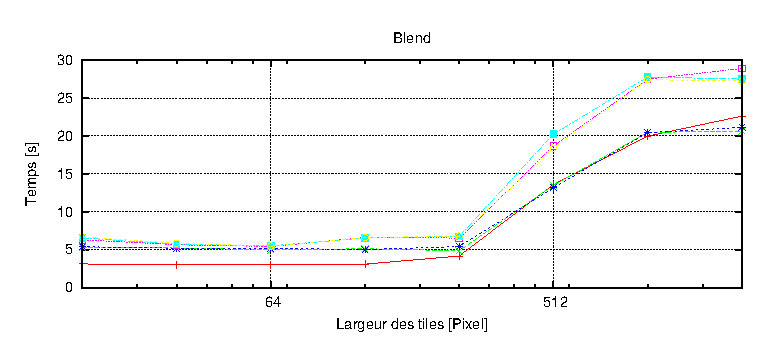
\includegraphics[width=\textwidth]{images/tilegraph.eps} 
				\label{fig:tilegraph}
			\end{figure}
		\subsubsection{Analyse des performances}
			On peut tirer plusieurs conclusion de ces expériences:
			\begin{itemize}
				\item Les tiles doivent être les plus grands possibles, pour diminuer le 
			nombre d'appels de fonctions, mais ne doivent pas être trop grands, sinon les performances sont très fortement dégradées. 
				\item Les tiles à canaux séparés sont jusque 2 fois plus lents que les tiles normaux.
				\item Le schémà d'accès aux tiles en mémoire a un impact non négligable mais plus marqué sur les tiles normaux.
				\item Le temps pour faire la fusion d'un même nombre de pixels peut différer de 970\% selon le type de tile, sa taille et la
				manière dont il est utilisé, puisque cette opération représente la grande majorité du temps de calcul du framework, ce choix
				est particulièrement important.
			\end{itemize}
			Enfin, il ne faut pas oublier que ces expériences ommettent deux facteurs importants: Le fait que la gestion des tiles dans le framework 
			est bien plus lourde, ce qui favorise les tiles plus grands, et le fait que les tiles plus petits permettent plus de précision dans 
			la localisation des opérations, ce qui permet de réduire le nombre de pixels accédés à chaque opération.

			Déterminer l'importance de ces deux facteurs requiert d'avoir des données d'utilisation du framework représentatives, par exemple
			avec des tests utilisateur. 
		\subsubsection{Structure finale}
			Le choix s'est porté sur des tiles normaux de taille fixe de $32\times32$ pixels, et ce quelque soit le modèle colorimétrique utilisé.
		\subsection{Les Frames}
			La Frame est la structure de donnée qui organise les tiles. Elle a deux utilités: Représenter une image bitmap et servir de cache aux
			résultats des opérations. La Frame est en fait une pyramide de tiles creuse, implémentée par des Quad-Trees.
			\subsubsection{Les Quad-Trees}
				Les Quad-Trees sont composés de FrameNodes. Ceux-ci sont une référence optionelle vers un tile, et quatre références, optionelles,
				vers des noeuds enfants. La tile référencée par le noeud représentant les quatres tiles des noeuds enfants à une échelle deux
				fois plus petite.

				Chaque ensemble de noeuds de la même profondeur représente ainsi un bitmap à l'échelle deux fois plus petite que l'ensemble de
				noeuds à la profondeur suivante.

			\subsubsection{Placer une image dans le Quad-Tree}
				Afin d'éviter d'avoir des Quad-Trees inutilement profond, les images sont stoquées au niveau le moins profond pouvant les contenir,
				soit $ceil( \log_2( max(size_x,size_y)/32))$, $size_x$,$size_y$ représentant la largeur et la hauteur de l'image en pixels.
				Cette profondeur est ensuite stoquée dans la Frame afin de pouvoir identifier le niveau de résolution native.

			\subsubsection{Référencer les Tiles dans le Quad-Tree}
				Les tiles sont référencés par trois coordonnées $(t_x,t_y,t_z)$. $t_x,t_y$ représente les coordonnées spatiales du tile, $t_x$ valant
				zéro à l'extrémité gauche du bitmap, et étant positif à droite. $t_y$ vaut zéro à l'extrémité supérieure du bitmap et est positif vers le bas,
				et ce quelque soit l'échelle représentée.
				
				$t_z$ représente le niveau d'échelle. Il vaut $0$ au niveau le plus profond, correspondant à la résolution native, et est positif
				pour les échelles inférieures. En effet, si l'on aggrandit ou réduit l'image, on modifie la profondeur du quad-tree, et donc la profondeur à 
				laquelle se trouve la résolution native. Cette définition du $t_z$ permet donc de référencer les tiles de l'image indépendemment de leur taille.
				
				Sa valeur maximale dépend donc de la taille de l'image stockée
				dans la Frame. Cependant, comme nous voulons pouvoir indexer les pixels indépendemment, la largeur de l'image ne peut dépasser
				\emph{MAX\_INT}, Ce qui correspond à une valeur maximale de $t_z$ de $26$ sur les architectures 32bits, avec des tiles de 32 pixels
				de coté.
				
			\subsubsection{Les coordonnées négatives}
				Lorsque la Frame sert à stocker un bitmap chargé depuis le disque, les pixels le constituant, et donc les tiles, sont toujours
				à des coordonnées positives. Cependant, il est pratique de pouvoir également stocker des pixels de coordonnées négatives, afin
				de disposer du plan complet pour pouvoir stocker le résultat de transformations géométriques. Pour ce faire, la Frame
				stoque un Quad-Tree par quadrant, et les tiles aux coordonnées négatives sont redirigées vers les Quad-Tree correspondant.

			\subsubsection{Le Tile de fond}
				Lorsque la frame est utilisée pour contenir un bitmap, celle-ci dispose d'un Tile de fond. Celui-ci n'est pas repris
				dans les Quad-Tree et est d'une couleur unie correspondant au 'fond' de l'image, habituellement une couleur transparente.
				Lorsque l'on tente d'accéder à une coordonnée qui ne correspond à aucun noeud des Quad-Trees, ce que l'on a atteint une zone
				correspondant au fond de l'image, et le tile de fond est renvoyé. Ceci permet de réduire l'espace pris par des zones vides
				de l'image.

		\subsection{Image}
		\subsection{Opérations}
		\subsection{États}
	\section{Algorithmes}
		\subsection{Rasterisation}
		\subsection{Dessin}
		\subsection{Sauvegarder l'état}
		\subsection{Charger un état}
		\subsection{Supprimer un état}
		\subsection{Modifier une opération}
	\section{Gestion de la cache}
	\section{Utilisation}
		\subsection{API publique}
		\subsection{Undo / Redo}
		\subsection{Modèle objet par calques}
		\subsection{Modèle objet nodal}
		\subsection{Traits de pinceau}

\chapter{Localité des operations (20 pages)}
	\section{Opérations vectorisées}
		\subsection{Impact sur l'API}
		\subsection{Évaluation des performances}
	\section{Bounding Boxes}
		\subsection{Algorithme Inline}
		\subsection{Algorithme Off-line}
		\subsection{Multi-Niveaux}
		\subsection{Impact sur l'API}
		\subsection{Évaluation des performances}

\chapter{Anti-aliasing (15 pages) }
	\section{Primitive de dessin}
	\section{Problèmes d'échelle}
		\subsection{Oversampling}
	\section{Problèmes de superposition}
	\section{Problèmes de bandes}
	\section{Problème de blending à faible opacité}
	\section{Problème de précision de positionement}
\chapter{Test utilisateurs (10 pages) }
	\section{Procédure}
	\section{Résultats}
	\section{Analyse}
\chapter{Comparaison d'Himalaya aux autres frameworks}
\chapter{Conclusion}

	
\chapter*{Abstract}
	\begin{abstract}
	Les images gigapixel ont un grand nombre d'applications, de l'art à la médecine en passant par la cartographie. Et plus 
	récemment, les jeux vidéos. Les techniques photographiques permettant de les générer ne manquent pas, l'espace stockage 
	et la bande passante non plus. Cependant les possibilités d'édition et de retouche numérique étaient jusqu'à présent 
	très limitées, aucun framework d'édition d'image ne se révélant satisfaisant. Une ébauche d'un nouveau concept de framework,
	conçu et réalisé par l'auteur, promettait des performances quasi indépendantes de la taille de l'image éditée, permettant ainsi 
	l'édition interactive d'images gigapixel

	Afin de vérifier ces promesses, l'implémentation du framework fut partiellement complétée, afin de se concentrer sur un problème restreint;
	la peinture d'images gigapixel. Cela révéla des problèmes de qualité et de performances,
	qui furent pour la plupart résolus de manière satisfaisante. Un logiciel de peinture utilisant ce framework fut ensuite 
	complété puis testé par 3 professionnels de l'art numérique afin d'évaluer la performance du framework et de son implémentation. 

	Les tests se sont conclus par la satisfaction des testeurs et la réalisation de plusieurs peintures gigapixel. 
	
	De nombreuses fonctionnalités du framework restent cependant à implé\-menter et à tester, de même que de nombreuses pistes
	d'amélioration des performances ont été ouvertes et restent à explorer.
	\end{abstract}
	

\chapter*{Préface}
	Ce rapport présente le résultat de mon mémoire réalisé au département de recherche en infographie de la \emph{Katholieke Universiteit Leuven}.
	Ce mémoire est également la conclusion de mon master d'ingénieur en informatique à L'\emph{Université Catholique de Louvain}.

	J'aimerais remercier les personnes suivantes: Philip Dutré de la KUL, et Marc Lobelle de l'UCL pour avoir été mes promoteurs,
	et Benedict J. Brown pour les avoir assisté dans cette tâche. J'aimerais également remercier les mémorants du département de recherche en infographie
	de la KUL pour leurs discussions et commentaire à propos de ce mémoire. 

	Enfin j'aimerais remercier Brice Vandemoortele, Jean-François Brogniet et Jean-Philippe Servais pour avoir participé aux tests utilisateur.

\chapter{Introduction}
	Les images gigapixel sont des images bitmap constituées de plus d'un milliard de pixel. Ces images apparaissent dans plusieurs domaines: la cartographie,
	avec les photographies satellites; la médecine, avec les images issues des microscopes; l'histoire et la préservation de l'art, avec des scans haute 
	résolutions de tableaux et fresques de grande taille; L'art numérique et également les jeux-vidéo qui utilisent de telles images pour la création
	de larges environnements. 

	Les algorithmes de compression et le faible coût de l'espace disque permettent de stocker sans encombre de telles images. Il existe également des logiciels
	de visualisation efficace. Cependant, lorsqu'il s'agit de les éditer, les logiciels existant ne proposent qu'une sélection très réduite des fonctionnalités
	proposées habituellement pour l'édition d'image mégapixel.  

	L'édition de telles images requiert une approche et des algorithmes différents. C'est ce que propose le framework nommé \emph{Himalaya}, conçu et
	partiellement implémenté au préalable par l'auteur de ce mémoire.  \emph{Himalaya} est un framework conçu pour pouvoir proposer la plupart des
	fonctionnalités des frameworks existants, avec des performances quasi indépendantes de la taille de l'image à éditer. 

	Cependant il y a un pas entre la conception et la réalisation, pas que nous avons partiellement franchi avec ce mémoire. En effet, l'implémentation
	complète du framework est une tâche d'une trop grande ampleur pour être envisagée ici. Nous avons donc fait le choix de se concentrer sur un
	sous-problème difficile, qui est de permettre de peindre de manière interactive une image gigapixel, fonctionnalité qui n'est proposée par aucun
	framework existant.

	Avant d'examiner en détail le framework \emph{Himalaya} il est important de se demander ce qu'est un framework d'édition d'image, quelles sont les
	fonctionnalités utiles et nécessaires de ceux-ci. Enfin il faudra regarder de quelle manière les frameworks existants proposent ces fonctionnalités,
	afin de comprendre les enjeux de conception. C'est ce que nous allons faire au prochain chapitre. 
	
	
\chapter[Présentation des frameworks d'édition d'images][Frameworks d'édition d'images]{Présentation des frameworks d'édition d'images}
	

	Un framework est une librairie présentant une interface logicielle permettant à un utilisateur d'éditer des images. 
	
	\index{Framework d'édition d'images}
	Le terme utilisateur sera employé pour désigner en toute généralité des choses assez différentes. Ainsi il désignera parfois 
	l'artiste qui utilise le logiciel d'édition, le programmeur qui utilise le framework pour
	concevoir un logiciel, mais aussi un autre programme qui ferait appel à celui ci.  

	Nous allons tout d'abord examiner quels sont les éléments qui constituent un tel framework, ensuite quels sont
	les fonctionnalités qu'ils doivent présenter à l'utilisateur. 

	Ensuite un survol des différents frameworks permettra des principes généraux de la conception d'un framework d'édition d'image.
	
	Pour réaliser cette présentation je me suis basé sur une lecture du code source des différents frameworks open-source, afin d'évaluer
	les structures de données et les algorithmes utilisés. J'ai également étudié les fonctionnalités et performances des logiciels fermés,
	qui bien que gardant secret leur fonctionnement, proposent généralement de meilleures performances et un plus large panel de fonctionnalités.
	
	Enfin, une étude des spécifications des principaux formats de fichiers standards permet de se rendre compte des fonctionnalités qui sont 
	attendues dans les frameworks. 

	Après chaque description de chaque framework on trouvera la liste des formats et logiciels ainsi examinés.

	\section{Architecture d'un framework d'édition d'image}
		Un framework d'édition d'images est composé de trois éléments principaux : 
		\begin{description}
			\item[Schéma de représentation de l'image]: Ce schéma est constitué de structures de données qui 
			décrivent l'image et les modifications qui lui sont apportées. 
			\item[Algorithme de rasterisation]: Cet algorithme permet d'obtenir une version matricielle de l'image,
			ou d'une partie de celle-ci. Une telle opération est indispensable car seule la forme matricielle de l'image
			peut être affichée à l'écran.
			\item[Algorithmes d'édition du schéma]: Ces algorithmes vont modifier la représen\-tation de l'image afin 
			d'implémenter les différentes fonctionnalités du framework.
		\end{description}

	\section{Fonctionnalités d'un framework d'édition d'image}
		\subsection{Opérations de dessin}
			L'opération de base d'un framework d'édition d'image est bien évidemment de permettre de 
			modifier une image. On distingue plusieurs manières de le faire qui seront traitées différemment
			selon les implémentations.
			\subsubsection{Dessin de primitives}
				Par dessin de primitive on entend l'ajout sur l'image de primitives géométriques, comme
				des polygones, des lignes, des points, des ellipses, du texte, etc. Ces primitives ont généralement un 
				effet local sur l'image, c'est à dire qu'elles ne la modifient pas dans son intégralité. 

				On différencie deux approches du dessin de primitive: L'approche dite vectorielle ou l'on utilise un 
				nombre réduit de primitives complexes (texte, courbes de bézier,...), et l'approche bitmap ou l'on utilise
				un très grand nombre de primitives très simples(ellipses, petits bitmaps, ...) qui prennent peu ou pas
				de ressources. 

				L'approche vectorielle permet de décrire facilement et efficacement des images très structurées, telles
				que des document textes, des graphes, des schémas techniques, ou des dessins schématisés. 

				Les techniques de graphe de scène (voir la section \emph{Frameworks Vectoriels}) s'adaptent très bien
				à cette approche et permet de structurer ces images de manière spatiale et sémantique.

				Le nombre quasiment illimité de primitives que permet la seconde approche rend possible la description
				d'images totalement déstructurées telles que les peintures.

				Puisque nous voulons développer un framework de peinture d'images gigapixel, c'est vers cette
				seconde approche que nous devons nous tourner. 

				\index{Primitives, dessin de}
				\begin{figure}[h]
					\centering
					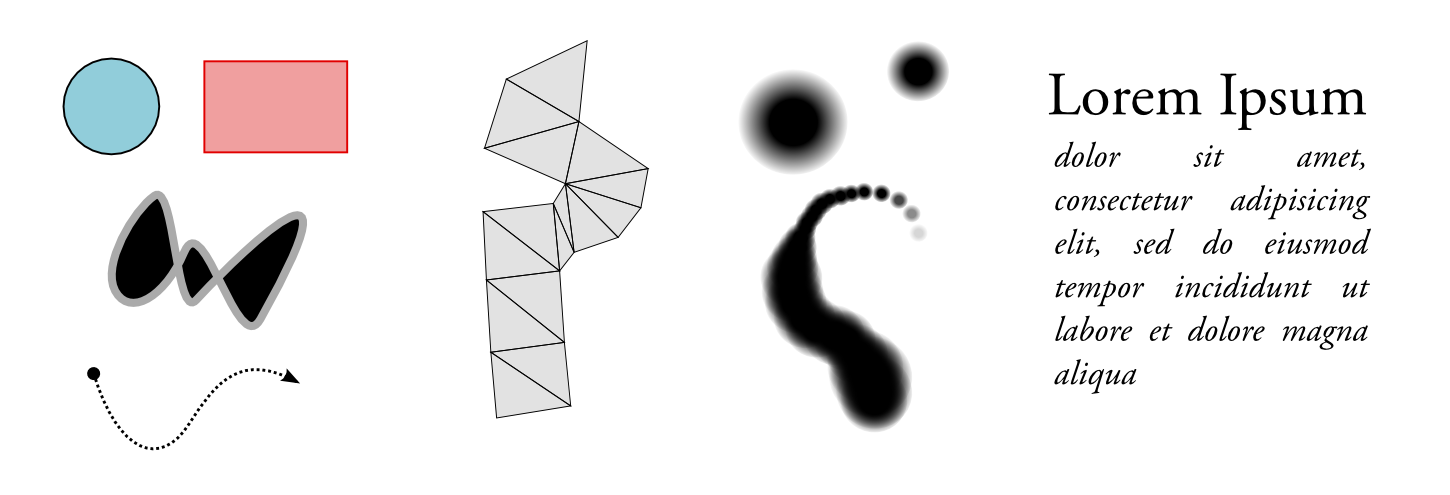
\includegraphics[width=\textwidth]{images/primitives}
					\caption{Exemples de dessins de primitives}
					\label{fig:primitives}
				\end{figure}
			\subsubsection{Filtres}
				\index{Filtres}
				Un filtre est une opération qui modifie l'aspect de l'entièreté d'une image. Le temps de calcul d'un filtre varie
				énormément d'un filtre à l'autre. Les plus simples prennent quelques microsecondes et peuvent aisément être exécutés
				en temps réel. D'autres prennent plusieurs dizaines de minutes\footnote{Un exemple récent est le \emph{Content Aware Filling}, \cite{contentaware}}. Certains frameworks ne sauront intégrer que les filtres
				les plus rapides. 

				Les filtres peuvent être également partagés en deux catégories,\index{Filtres!colorimétriques} les filtres colorimétriques qui transforment
				la couleur d'un pixel sans se soucier de la couleur des pixels voisins, \index{Filtres!spatiaux} et les filtres spatiaux nécessitant 
				eux d'en connaître plusieurs. 
				\begin{figure}[h]
					\centering
					\subfloat[Image originale]{ \label{fig:lenna_a} 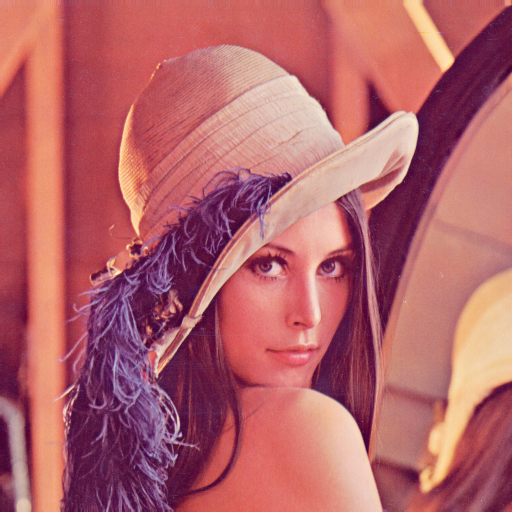
\includegraphics[width=0.3\textwidth]{images/Lenna} }
					\subfloat[Filtre colorimétrique]{ \label{fig:lenna_b} 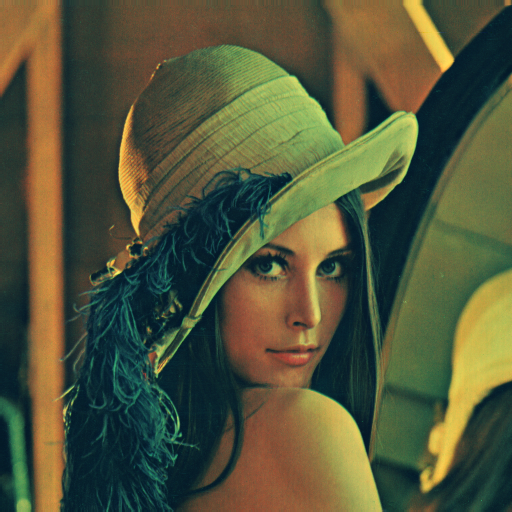
\includegraphics[width=0.3\textwidth]{images/Lenna-green} }
					\subfloat[Filtre spatial \emph{Sobel}]{ \label{fig:lenna_c} 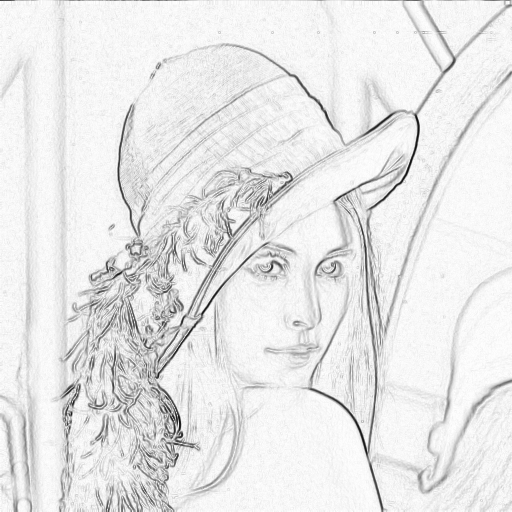
\includegraphics[width=0.3\textwidth]{images/Lenna-sobel} }
					\caption{Exemples de filtres}
					\label{fig:filtres}
				\end{figure}
			\subsubsection{Transformations géométriques}
				Les transformations géométriques modifient la forme d'un objet constituant l'image; rotation, translation, 
				redimensionnement et perspective sont les applications les plus courantes. 
				
				Il y a deux approches pour implémenter les transformations
				géométriques: l'approche vectorielle consiste à modifier la description de l'image avant la rasterisation. L'approche
				bitmap consiste à modifier les pixels après leur rasterisation. Cette deuxième approche, nettement plus lente, permet
				cependant d'implémenter des transformations non linéaires, telle que les transformées polaires, la correction de distorsion de 
				lentille, ou les déformations fluides. 
				
			\subsubsection{Fusion et modes de fusion}
				La fusion consiste à fusionner deux images en une. On utilise pour cela une fonction nommée \emph{mode de fusion}.
				Elle à la forme $f(p_A ,p_B ,\alpha)$, où $p_A$, $p_B$ sont deux pixels des images $A$,$B$ que l'on veut fusionner. 
				$\alpha$ représente un ou plusieurs paramètres additionnels qui peuvent	modifier l'effet de la fonction.

				Le \emph{mode de fusion} la plus courante est celui de mélange par opacité: $f(p_A, p_B, \alpha) = \alpha * p_A + (1-\alpha) * p_B$,  $\alpha \in [0,1]$ 
				représentant l'opacité de $B$, mais il en existe bien d'autres.

				On peut utiliser cette fonction pour fusionner deux images en une nouvelle : $ C = f(A,B,\alpha)$, ou pour intégrer une image dans
				une autre $A = f(A,B,\alpha)$

				Puisque chaque dessin de primitive consiste en la fusion de celle ci sur l'image de fond, la fusion est une opération centrale
				dans tout framework. Cependant beaucoup d'entre eux se limitent au seul mode de mélange par opacité.

				\begin{figure}[h]
					\centering
					\subfloat[Image A]{ \label{fig:A} 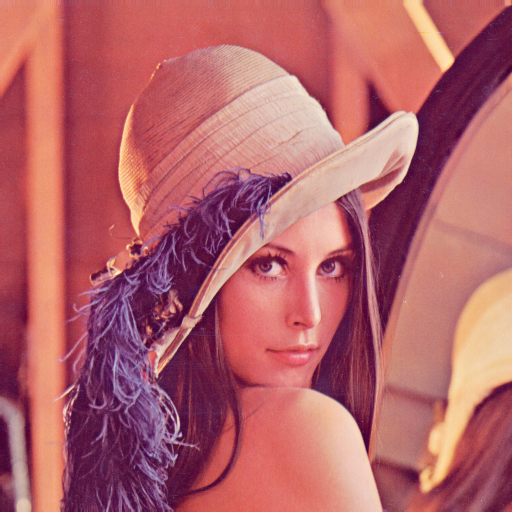
\includegraphics[width=0.25\textwidth]{images/Lenna} }
					\subfloat[Image B]{ \label{fig:B} 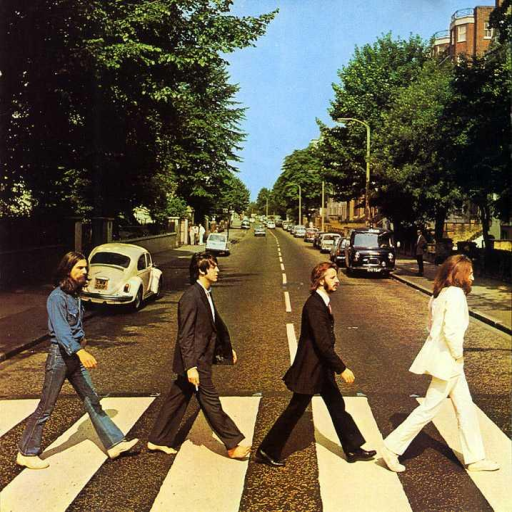
\includegraphics[width=0.25\textwidth]{images/abbey-road} }
					\subfloat[Blending de B sur A, par \emph{fusion de grain} ]{ \label{fig:ABfusion} 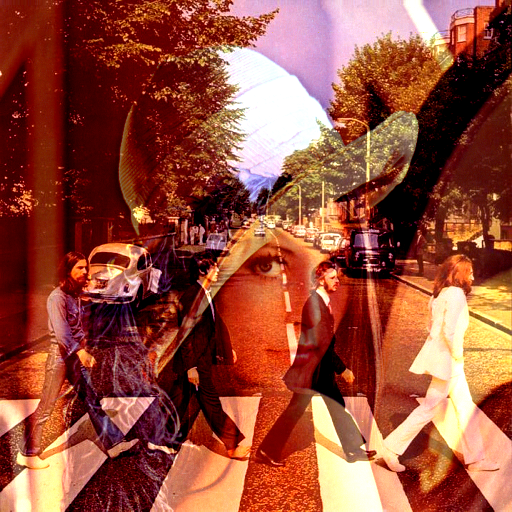
\includegraphics [width=0.25\textwidth]{images/abbey-road-lenna-fusion} }
					\subfloat[Blending de B sur A, par \emph{soustraction} ]{ \label{fig:ABsoustraction} 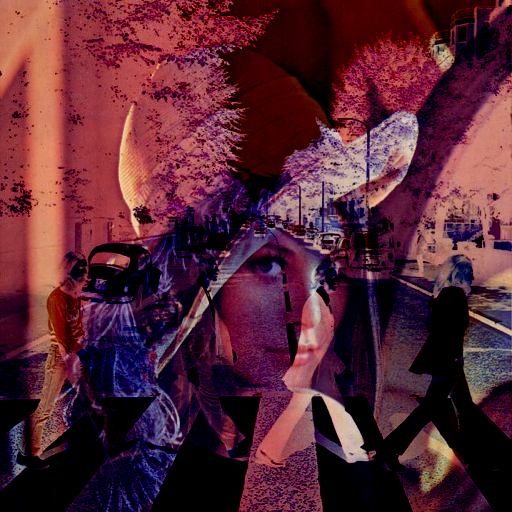
\includegraphics [width=0.25\textwidth]{images/abbey-road-lenna-substract} }
					\caption{Exemples de blending}
					\label{fig:blending}
				\end{figure}

		\subsection{Modèles colorimétriques}
			La rasterisation d'une image permet de définir la couleur de chaque pixel. Or il existe de nombreuses manières de définir une même couleur.
			La manière la plus populaire est de définir la couleur comme un vecteur dans un espace colorimétrique. Chaque espace ayant sa propre utilité:
			\begin{description}
				\item[Le RGB] est l'espace utilisé par les écrans et projecteurs, ainsi que les capteur photographiques. Toute couleur doit donc être
				convertie en RGB avant d'être affichée. Il existe plusieurs espaces RGB définis par des couleurs primaires Rouges, Vertes et Bleues différentes.
				Le plus utilisé est le sRGB, qui est le standard d'affichage des écrans\cite{reviewrgb}.
				\item[Le Yuv] est l'espace utilisé par les vidéos et par certains formats de fichier comme le JPEG.
				L'espace Yuv permet en effet une meilleure compression des données.
				\item[Le CIELab] est l'espace utilisé en retouche photo, il permet de manipuler les couleurs de manière conforme à la perception humaine.
				\item[Le HSL] est un espace qui permet de décrire les couleurs en composantes de teintes, de saturation et de luminosité, notions
				facilement compréhensibles et manipulables. Cet espace est utilisé pour certains filtres et pour l'édition des couleurs.
				\item[Le CMYK] est l'espace utilisé par les imprimantes jet d'encre, chaque imprimante ayant ses propres couleurs primaires. 
				Toute image doit donc être convertie dans le CMYK correspondant à l'imprimante avant d'être imprimée.
			\end{description}
			Il existe encore bien d'autres espaces colorimétriques spécifiques à des applications industrielles particulières. 

			Pour compliquer le tout, les espaces colorimétriques ne se superposent géné\-ralement pas. Ainsi des couleurs qui peuvent s'exprimer dans l'un n'existent pas
			dans l'autre. Un framework dédié à l'impression doit ainsi prendre garde de n'afficher en RGB que des couleurs disponibles dans le CMYK de l'imprimante.

			Une autre manière de décrire les couleurs est d'utiliser un nuancier contenant une liste de couleurs standardisées. Ce système est utilisé dans les images destinées à l'impression
			afin d'identifier des encres dont l'apparence ne peut être réduite à une simple couleur, comme les encres mattes, brillantes, métallisées,
			fluorescentes, etc. Dans ce cas chaque pixel possède une certaine quantité de chacune des  couleurs utilisées pour décrire l'image.

			\subsubsection{Quantisation}
			Les composantes d'un pixel peuvent aussi être quantifiées à différents degrés: 1bit pour les systèmes halftone; 8bit pour l'affichage 
			à l'écran,  les textures de jeux-vidéo; 32 bit flottant pour avoir des valeurs de couleurs dépassant les capacité d'affichage
			d'un écran, ce qui est particulièrement intéressant pour l'édition non destructive d'image utilisée en photographie et en 
			effets spéciaux. La précision apportée par une telle profondeur est également indispensable pour le cinéma numérique.

			\subsubsection{Extensions de modèles colorimétriques}

			Enfin, il arrive qu'un pixel ne décrive plus une couleur mais une information quelconque de la partie de l'objet qu'il représente.
			On rencontre ainsi la distance du pixel à l'observateur, la normale de la surface, un identifiant unique de l'objet, la vitesse de
			déplacement de l'objet, etc. Ces informations sont généralement fournies en plus des informations colorimétriques habituelles.

			Ce type d'information est typiquement fourni par la caméra ou généré par le moteur de rendu afin de faciliter l'intégration d'effets
			spéciaux à l'image. Les types d'informations utilisés apparaissent et disparaissent avec les technologies, nécessitant une grande 
			flexibilité dans leur gestion. Les \emph{Éditeurs Nodaux} sont particulièrement adaptés à la gestion de ce type d'informations.
			
			\begin{figure}[h]
				\centering
				\subfloat[Couleurs vraies]{ \label{fig:render} 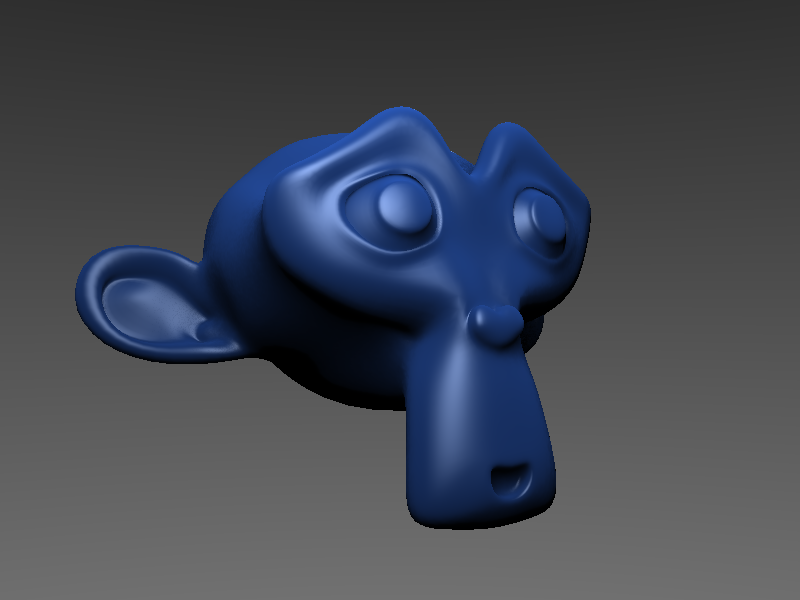
\includegraphics[width=0.25\textwidth]{images/render} }
				\subfloat[Format HSL en fausses couleurs]{ \label{fig:render-hsv} 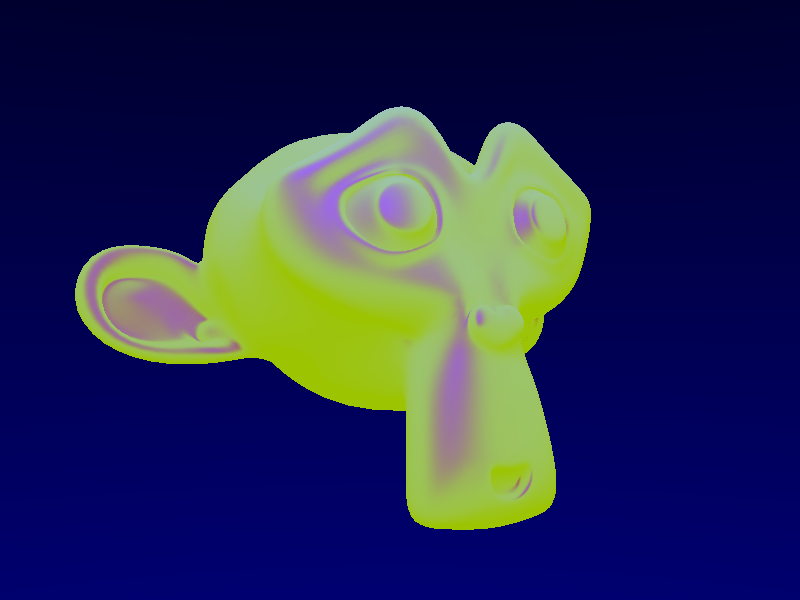
\includegraphics[width=0.25\textwidth]{images/render-hsv} }
				\subfloat[Vecteur normal de la surface]{ \label{fig:render-normal} 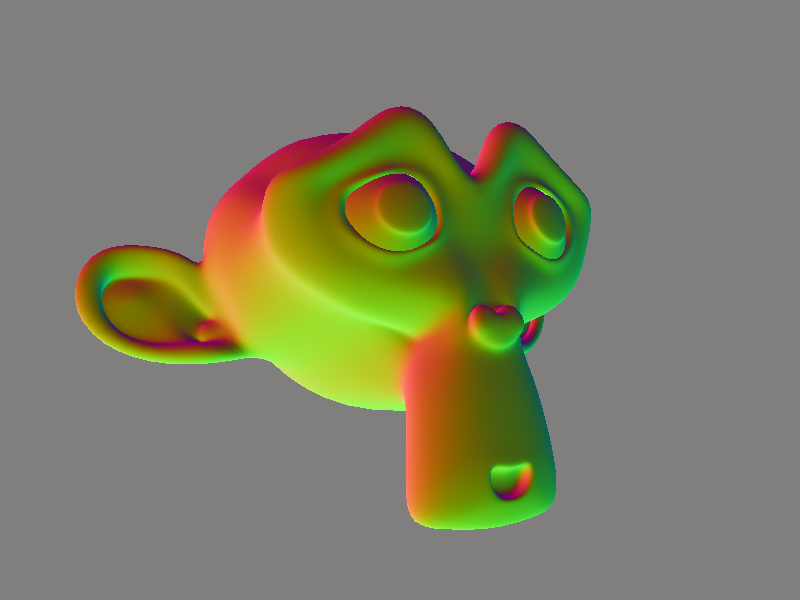
\includegraphics [width=0.25\textwidth]{images/render-normal} }
				\subfloat[Distance à l'observateur]{ \label{fig:render-depth} 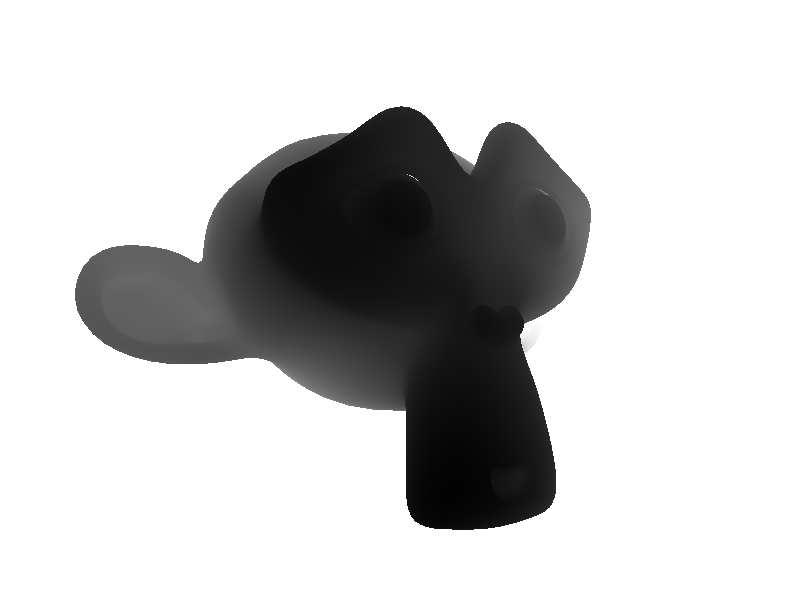
\includegraphics [width=0.25\textwidth]{images/render-depth} }
				\caption{Exemples d'espaces colorimétriques et de méta-données}
				\label{fig:color}
			\end{figure}

		\subsection{Undo / Redo}
			Un framework a souvent des mécanismes internes permettant une gestion efficace d'annulation et de répétition des opérations.
		\subsection{Édition non destructive}
			L'édition non destructive consiste à pouvoir modifier les opérations après leur application sans perte de qualité de l'image.
		\subsection{Composition non linéaire}
			La composition non linéaire permet à une opération d'utiliser le résultat d'une opération autre que celle appliquée précédemment. Idéalement
			le résultat de cette opération ne doit pas être recalculé. Cette fonctionnalité permet de combiner des effets simples afin d'obtenir des
			effets beaucoup plus complexes que ce qui est possible par composition linéaire, et permet souvent à l'utilisateur d'éviter de devoir 
			programmer ses propres effets. De nombreux logiciels présentent ainsi une interface nodale 
			comme alternative à la programmation de pixel-shaders.

		\subsection{Édition par pixel}
			Certains frameworks permettent d'éditer individuellement chaque pixel de l'image. 
		\subsection{Indépendance à la résolution}
			La description de l'image est indépendante de la résolution utilisée pour la rasterisation; Il n'y a pas de dégradation
			de la qualité de l'image quelque soit la résolution utilisée pour le rendu. L'édition par pixel et l'indépendance à la résolution
			sont deux fonctionnalités mutuellement exclusives.
		\subsection{Images gigapixels}
			Les images gigapixels sont les images constituées de plus d'un milliard de pixel, qui peuvent être plus grandes que la mémoire
			vive disponible. Il ne faut pas confondre édition d'images gigapixel et indépendance à la résolution.
			Si l'indépendance à la résolution permet de décrire des documents de tailles aussi grande
			que désirée et de les rasteriser en des images gigapixel, elle ne permet pas de décrire ou d'éditer des images
			de plus d'un milliard de pixels indépendants. 

		\subsection{Traitement d'images multiples}
			Le traitement d'images multiples consiste à savoir appliquer facilement les mêmes opérations sur un large nombre d'images similaires, 
			comme par exemple les photos d'une séance de shooting, les frames d'une vidéo ou d'un moteur 3D.

	\section{Frameworks Bitmaps}
		\subsection{Schéma de représentation de l'image}
			\begin{figure}[h]
				\centering
				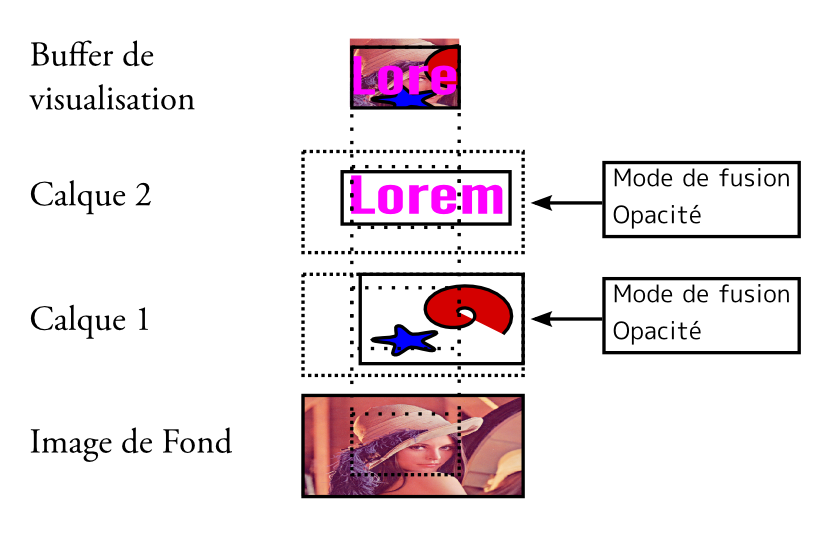
\includegraphics[width=0.6\textwidth]{images/calques}
				\caption{Représentation d'une image par calques}
				\label{fig:editbitmap}
			\end{figure}
			Dans un framework bitmap l'image est représentée directement sous sa forme rasterisée. 
			
			Une extension populaire est de décomposer l'image en une image de fond et une superposition de calques qui sont des bitmaps possédant chacun leur propre
			dimension, position, un mode de fusion, et des paramètres d'opacité. Cette extension permet à l'utilisateur de pouvoir facilement modifier des zones
			spécifiques de l'image.

			Des frameworks étendent encore ce principe en décomposant les calques en sous calques, et ce de manière récursive\footnote{Un exemple de logiciel proposant cette fonctionalité est \emph{Adobe Photoshop}}. 

		\subsection{Algorithme de rasterisation}
			Dans un framework bitmap, chaque opération est directement rasterisée à la résolution native lors de son application. 
			
			Pour visualiser une région à une échelle différente de la résolution native, On utilise un buffer de visualisation de la taille
			de cette région dans lequel la région d'intérêt est mis à l'échelle voulue après chaque rasterisation.
			
			Lorsqu'un système de calques est utilisé, on rasterise d'abord directement l'opération sur le calque modifié. On place ensuite l'image
			de fond dans le buffer de visualisation. Chaque calque y est ensuite fusionné.			
			
			Comme la plupart des opérations ne modifie qu'une petite partie de l'image, on aimerait éviter de devoir fusionner l'intégralité
			des calques à chaque fois. Il y a deux approches pour cela: La première est de demander à chaque opération de spécifier la région
			qu'elle modifie. On ne modifie ensuite le buffer de visualisation que pour cette région. 

			La deuxième approche consiste à diviser l'image de fond et les calques en une grille de sous régions aux dimensions régulières appelées
			tiles. Lors de l'application de l'opération, celle ci ne modifiera que certains tiles. Seuls les tiles correspondants dans les calques
			et l'image de fond seront fusionnés dans le buffer de visualisation. Les tiles peuvent également être traités en parallèle sur une 
			machine multiprocesseur.

			Les tiles ont d'autres intérêts que d'accélérer la rasterisation; En omettant les tiles des zones transparentes des calques ou réduit 
			l'espace mémoire qu'ils consomment. En outre, les tiles peuvent être migrés vers le disque dur lorsqu'il n'est plus possible de tous
			les stocker en mémoire, ils sont ensuite récupérés lorsqu'ils sont utilisés. 
			
			Il n'est cependant pas toujours possible d'implémenter une opération pour qu'elle fonctionne tile par tile. Dans ces cas on devra placer
			les tiles dans un buffer temporaire et les récupérer après l'opération. 

		\subsection{Fonctionnalités adaptées aux frameworks bitmaps}
			\subsubsection{Opérations de dessin}
				Étant donné qu'il n'est pas nécessaire de maintenir une liste de toutes les opérations appliquées sur l'image, les frameworks
				bitmaps sont particulièrement efficaces lorsqu'un très grand nombre de celles-ci sont utilisés ce qui est le cas pour les
				logiciels de peinture. 
			\subsubsection{Undo / Redo}
				L'undo/redo est implémenté en gardant une copie de la région/tiles modifiée par l'opération avant sa modification. 
				Il suffit ensuite de réutiliser ces copies pour obtenir la version sauvegardée. Garder les copies consomme beaucoup de mémoire,
				et une limite d'historique est nécessaire pour pallier à ce problème. En revanche, annuler ou refaire une opération ne demande
				pas de recalculer l'opération et est donc très rapide.
		\subsection{Fonctionnalités inadaptées aux frameworks bitmaps}
			\subsubsection{Modèles colorimétriques et méta-données}
				L'architecture des frameworks bitmaps limite sévèrement les possibilité de gestion de modèles colorimétriques et de méta-données.
				En effet, comme chaque opération est rasterisée dans le calque dès son application, les opérations doivent nécessairement 
				avoir le même modèle colorimétrique en entrée et en sortie. Elles doivent aussi comprendre le modèle colorimétrique et extensions du 
				calque, ce qui nécessite de devoir soit modifier les opérations à chaque ajout de nouveau type de modèles colorimétriques et d'extensions
				soit de passer par de coûteuses transformations de modèles.

				Il existe une solution permettant d'améliorer la situation : Au lieu de placer tous les composants du pixel dans un même calque, on
				divise le calque en sous calques appelés canaux qui contiennent chacun un seul composant du pixel. Les opérations sont ensuite 
				codées pour prendre des canaux en entrée et en sortie. Il est maintenant possible d'ignorer les canaux inutiles, d'avoir des canaux
				de différentes précision, et de changer la signification d'un canal lors de l'application d'une opération. 

				Cette approche à pour inconvénient de ralentir nettement les opérations, puisqu'il faut désormais accéder des zones de 
				mémoire fort éloignées pour lire ou modifier un seul pixel. 

				En pratique les framework bitmap implémentent un nombre limité de modèles colorimétriques, et imposent
				le même modèle pour tous les calques d'une image\footnote{\emph{Gimp} est passé d'un framework bitmap à un framework nodal pour
				résoudre ce problème}
			\subsubsection{Images gigapixel}
				Il est théoriquement possible de gérer des images de taille plus grande que la mémoire disponible en utilisant les tiles à
				bon escient. Mais en pratique, chaque opération nécessite d'être appliquée intégralement sur l'image à résolution native, 
				ce qui est infaisable de manière interactive pour des opérations modifiant de grandes parties de l'image.
			\subsubsection{Édition non destructive}
				L'édition non destructive requiert de garder une liste de toutes les opérations effectuées sur l'image, afin de pouvoir
				modifier l'opération désirée, et de refaire celles qui doivent être ré-appliquées. 

				Il est cependant possible d'implémenter des opérations non destructives en tant que calques à part entière. 
				Si l'opération est un filtre spatial, il faudra pouvoir étendre le buffer de rasterisation pour que le filtre ait accès aux données
				nécessaires. Et s'il s'agit d'un filtre de transformation, la zone à modifier dans le buffer de visualisation devra elle aussi
				être modifiée au fur et à mesure des filtres. Tout cela étant fort compliqué à implémenter, sans garantie de performances, 
				les frameworks confinent généralement l'édition non destructive aux filtres colorimétriques et dessin de primitives
				\footnote{\emph{Adobe Photoshop} propose des filtres non destructifs fort avancés. \emph{Gimp} est passé d'un framework
				bitmap à un framework nodal pour faciliter l'édition non destructive}.
		\subsection{Framework bitmaps, l'état de l'art}
			\begin{description}
				\item[Adobe Photoshop] Logiciel de peinture et retouche photo
				\item[Corel Painter] Logiciel de peinture
				\item[Artrage] Logiciel de peinture
				\item[Gimp $\leq$ 2.6] Logiciel de peinture et retouche photo open source
				\item[Krita] Logiciel de peinture et retouche photo open source
				\item[Blender3d] Utilisé pour la peinture de texture, Logiciel d'animation 3D.
				\item[psd] Format d'image de Photoshop
				\item[xcf] Format d'image de Gimp.
			\end{description}

	\section{Frameworks Nodaux}
		\subsection{Schéma de représentation de l'image}
			\begin{figure}[h]
				\centering
				\subfloat[En rouge les noeuds d'entrée, en orange les noeuds d'opération, en vert les noeuds de visualisation]{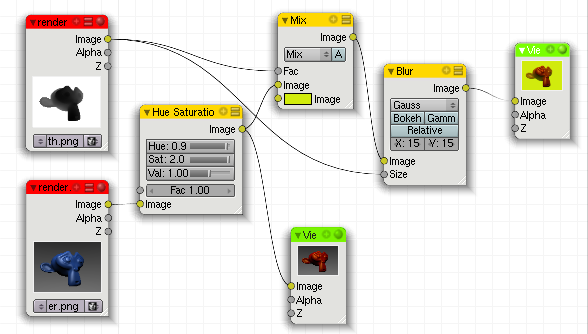
\includegraphics[width=0.8\textwidth]{images/nodes} }
				\\
				\subfloat[Image calculée par le graphe (a)]{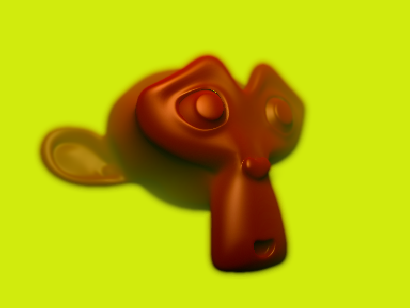
\includegraphics[width=0.4\textwidth]{images/nodes-out} }
				\caption{Exemple d'édition nodale d'images telle qu'implémenté par \emph{Blender 2.49}}
				\label{fig:editnodal}
			\end{figure}
			Les frameworks nodaux représentent l'image par un graphe composé de trois types de noeuds.
			\begin{itemize}
				\item Les noeuds d'entrée servent à spécifier les images à modifier et ne proposent que des sorties --- en rouge sur la figure~\ref{fig:editnodal}(a)
				\item Les noeuds d'opération --- en orange sur la figure~\ref{fig:editnodal}(a) --- prennent en entrée des images et/ou des canaux et/ou des paramètres,
				et proposent en sortie le résultat des images et/ou des canaux et/ou des valeurs, résultats de
				l'opération sur les entrées.
				\item Les noeuds de visualisation --- en vert sur la figure~\ref{fig:editnodal}(a) --- n'ont qu'une entrée et servent à visualiser sa valeur, que ce soit un paramètre,
				un canal ou une image. Dans le cas de canaux ou d'images, le noeud peut également spécifier une sous région
				de l'image et une échelle.
			\end{itemize}
			Le graphe est acyclique et dirigé; chaque arrête va de la sortie d'un noeud à une entrée d'un autre. Il peut
			y avoir plusieurs arrêtes partant d'une sortie, mais une seule arrivant à chaque entrée. 
		
		\subsection{Algorithme de rasterisation}
			Pour obtenir la sortie d'un noeud, il faut premièrement obtenir toutes ses entrées, et appliquer l'opération du
			noeud s'il y en a une. On appliquera donc ce principe de manière récursive en partant d'un noeud de visualisation,
			la récursion s'arrêtant au noeuds d'entrée.

			Si le noeud de visualisation spécifie une sous-région de l'image, l'algorithme fonctionne de manière identique, à
			ceci près que les opérations pouvant transformer géométriquement l'image, la région en entrée ne sera pas la même que
			la sortie. Il faut donc que le noeud soit capable d'inverser la transformation qu'il effectue afin de demander la bonne
			région à ses parents\footnote{Ce mécanisme est utilisé par le framework \emph{GEGL}.}. 

			Si le noeud de visualisation spécifie une échelle, les images fournies par les noeuds d'entrée sont mises à l'échelle avant
			leur sortie, de même que les paramètres métriques des opérations. 

			Comme une sortie peut être connectée à plusieurs entrées, une même opération peut être calculée plusieurs fois. Pour éviter
			cela, chaque noeud peut disposer d'une cache dans laquelle il place le résultat de ses sorties. 

			Les images utilisées peuvent également utiliser une représentation par tiles afin de bénéficier des avantages de gestion d'images
			volumineuses.

		\subsection{Fonctionnalités adaptées aux frameworks nodaux}
			\subsubsection{Édition non destructive}
				C'est un des gros points forts des frameworks nodaux. On peut facilement modifier les paramètres et la topologie du graphe
				et visualiser le résultat.
			\subsubsection{Composition non linéaire}
				La composition non linéaire découle de l'architecture en graphe des frameworks nodaux. Les frameworks nodaux sont d'ailleurs
				les seuls frameworks permettant une réelle édition non linéaire. 
			\subsubsection{Modèle colorimétrique}
				Un framework nodal offre une liberté totale à l'utilisateur en ce qui concerne les modèles colorimétriques. Si un noeud sort
				une image en RGB, et qu'une opération attend du YUV, il peut les connecter ensemble. Le canal R sera interprété comme Y, le G comme
				U et le B comme V\footnote{Ce mécanisme est implémenté dans \emph{Blender3d}}. S'il désire garder l'interprétation colorimétrique du RGB, il devra utiliser un noeud qui convertit le RGB en YUV.

				Intégrer un nouveau modèle colorimétrique se limite donc à créer des noeuds de conversions et les noeuds d'opération qui peuvent
				tirer bénéfice de ce nouveau modèle.

				L'édition nodale est cependant incapable de gérer les tons directs.
			
				
			\subsubsection{Images gigapixel}
				La complexité en temps et en mémoire de la rasterisation d'une image ne dépend tout au long du graphe que de la taille de
				la région du noeud de visualisation. Une borne supérieure de la taille de ces région est la résolution des écrans qui ne
				dépasse pas les quelques mégapixels. Il reste l'opération d'échelle à effectuer au niveau des région d'entrée. Si on
				dispose de mipmaps de ces images, alors il est possible d'effectuer des opérations sur images gigapixels de manière efficace
				\footnote{\emph{GEGL} implémente ce mécanisme}.
			\subsubsection{Traitement d'images multiples}
				Le même graphe peut très facilement s'appliquer sur un grand nombre d'images de manière automatique, ce qui rend ces frameworks
				particulièrement adaptés au traitement vidéo.
				
		\subsection{Fonctionnalités inadaptées aux frameworks nodaux}
			\subsubsection{Undo/Redo}
				On peut s'attendre d'un framework permettant l'édition non destructive d'exceller dans l'undo/redo. Cependant, il n'est pas
				facile de gérer les changements de paramètres des noeuds et de la topologie du graphe tout en maintenant des caches cohérentes.
				C'est pourquoi les graphes nécessitent souvent d'être rasterisés à nouveau ce qui peut prendre du temps lorsque celui ci contient
				des filtres complexes. 
			\subsubsection{Opération de dessin de primitives}
				Il est tout à fait possible de créer des noeuds dessinant des primitives, et de les connecter entre eux pour avoir une topologie
				semblant correspondre aux frameworks bitmaps ou vectoriels. 

				Un premier problème est que les frameworks nodaux appliquent les opérations de transformations sur les pixels constituant la primitive et non sur les paramètres la définissant.
				Par exemple, il sera impossible de récupérer l'apparence exacte de la primitive après une transformation d'échelle 
				la réduisant à un seul pixel. Cet exemple extrême démontre comment à chaque transformation successive, la primitive est peu à peu
				dégradée. Un framework vectoriel n'a pas ce genre de problèmes.
				
				Ensuite, un framework nodal est une entité complexe, et il devient impossible à l'utilisateur de gérer un graphe contenant 
				autant de noeuds que nécessiterait la réalisation d'une peinture. Sans parler de la consommation en mémoire du graphe, 
				et de la surcharge de calcul qu'entraîne le parcours de celui-ci.

				On ne peut pas non plus se permettre de devoir recalculer toutes les opérations de dessin à chaque Undo/Redo, à chaque édition
				non destructive et à chaque nouvelle visualisation.

				Les frameworks nodaux font donc souvent le choix d'ignorer totalement les opérations de dessin. Celles-ci sont alors effectuées
				sur les images avant leur entrée dans le graphe, et doivent être gérées par un autre framework tel qu'un framework vectoriel ou bitmap.

				Certains frameworks nodaux (GEGL) choisissent de proposer des noeuds qui regroupent une séquence d'opération de dessin en une seule.
				Ces noeuds sont donc obligés de gérer par des mécanismes interne l'undo/redo. De tels noeuds fonctionnant comme des frameworks bitmaps
				ils ne peuvent pas gérer des opérations de dessin de trop grande taille. 
				
				Ces frameworks permettent donc de peindre sur des images gigapixel, mais chaque trait de peinture doit rester de taille mégapixel,
				ce qui limite l'utilité de cette fonctionnalité dans le cadre d'édition d'images gigapixel.


			\subsubsection{Édition par pixel}
				L'édition par pixel est problématique pour les mêmes raisons qui rendent problématique le dessin de primitives.
		\subsection{Framework nodaux, l'état de l'art}
			\begin{description}
				\item[The Foundry Nuke]Logiciel de composition et post processing vidéo
				\item[Blender3D]Utilisé pour la composition et le post processing vidéo, logiciel d'animation 3D open source.
				\item[GEGL]Framework nodal open source utilisé par Gimp $\geq$ 2.7 et le logiciel d'acquisition numérique Gnome Scan.
				\item[OpenRaster]Format d'image public permettant de sauvegarder des graphes d'opérations et compatible avec GEGL.
			\end{description}

	\section{Framework vectoriel}
		\subsection{Schéma de représentation de l'image}
			\begin{figure}[h]
				\centering
				\subfloat[l'image]{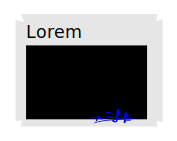
\includegraphics[width=0.33\textwidth]{images/scenegraph-img} }
				\subfloat[Le graphe de scène]{ 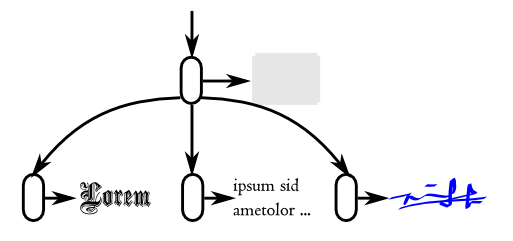
\includegraphics[width=0.66\textwidth]{images/scenegraph-graph} }
				\caption{Représentation d'une image par graphe de scène}
				\label{fig:scenegraph}
			\end{figure}
			L'image est décrite par un ensemble de primitives géométriques. Ces primitives sont organisées dans un graphe de scène. Dans un 
			graphe de scène, chaque noeud représente une transformation géométrique et une primitive. La transformation géométrique détermine
			la position, l'échelle, et la rotation de la primitive et de ses enfants. La primitive est elle décrite par son type et les paramètres
			qui déterminent sa forme et son apparence.

			Le graphe de scène est acyclique. chaque noeud peut avoir plusieurs enfants et sauf exception un seul parent. 

			L'ordre des enfants d'un noeud est important puisqu'ils déterminent l'ordre dans lequel ils seront dessinés. Ainsi les derniers
			enfants d'un noeuds seront dessinés au dessus des premiers. 

			Chaque framework a sa propre liste de primitives géométriques, mais tous disposent au moins de points, lignes, polygones, ellipses,
			texte, et courbes de bézier.

		\subsection{Algorithme de rasterisation}
			L'utilisateur commence d'abord par choisir la région qu'il veut rasteriser et à quelle résolution. Le framework crée ensuite un bitmap
			de cette taille et résolution de la couleur de fond de l'image.

			Pour dessiner un noeud du graphe, on applique sa transformation aux paramètres de sa primitive. On dessine ensuite cette 
			primitive sur le bitmap. On Dessine ensuite chaque noeud enfant dans l'ordre en leur appliquant la transformation de ce noeud.

			Cette opération est effectuée de manière récursive en partant du noeud racine de l'image.

			Afin d'éviter de dessiner les primitives qui se trouvent en dehors de la région à rasteriser, on associe à chaque noeud une boite
			qui englobe sa primitive ainsi que celles de tous ses enfants. Si la boite est en dehors de la région, on peut ignorer ce noeud et
			leurs enfants. 

			Afin d'exploiter l'accélération matérielle, la plupart des frameworks ne dessinent pas directement les primitives, mais les 
			convertissent en triangles qui sont ensuite dessinés à l'aide du matériel. Cette approche peut également s'avérer bénéfique 
			sans accélération matérielle car le dessin de triangle est souvent beaucoup plus rapide qu'un dessin analytique de la primitive,
			de plus les détails trop petits pour être vus peuvent être détectés lors de la transformation de la primitive en triangles.

		\subsection{Fonctionnalités adaptées aux frameworks vectoriels}
			\subsubsection{Édition non destructive}
				La description de la scène étant gardée en mémoire, il est facile de la modifier et d'obtenir ensuite une nouvelle visualisation.
				L'algorithme de rasterisation ne disposant généralement pas de cache\footnote{La librairie \emph{libart} est une exception notable. Il est également probable que certains frameworks fermés disposent égalemnt de systêmes de caches.}
			
				modification de l'image. Cela n'est pas un problème tant que la taille du graphe de scène reste raisonnable.
			\subsubsection{Undo / Redo}
				L'undo/redo est simple à implémenter et aussi efficace que l'édition non destructive. 
			\subsubsection{Opérations de dessin de primitives}
				Les frameworks vectoriels sont très pratiques pour éditer un dessin constitué de primitives géométriques. Cependant, la région de
				visualisation doit être rasterisée à chaque changement d'échelle ou à chaque déplacement de celle-ci. Si le nombre de primitives
				constituant le dessin est trop grand, cela ne peut plus se faire de manière interactive.
				
				Les frameworks vectoriels sont donc généralement utilisés pour les documents textuels, les cartes, les graphes, ou les dessins abstraits
				qui peuvent être décrits par un petit nombre de primitives complexes. A contrario, les images peintes utilisent 
				un trop grand nombre de primitives pour que de tels frameworks soient efficaces. 
		\subsection{Fonctionnalités inadaptées aux frameworks vectoriels}
			\subsubsection{Filtres}
				En associant les filtres aux noeuds on s'attend à ce que le filtre ne s'applique
				qu'à ce noeud et à ses enfants. Ceci nécessite de faire une rasterisation de ces noeuds dans un buffer séparé afin d'y appliquer le
				filtre, puis de réintégrer ce buffer dans le buffer en cours. Et ce de manière récursive selon qu'il y ait des filtres dans les
				noeuds enfants. 
				Tout cela ralentit nettement la rasterisation, d'autant que le rendu dans de multiples buffer ne fait pas bon ménage avec 
				l'accélération matérielle. Les frameworks proposent parfois de tels filtres, mais les performances suivent rarement.
				
				Le format vectoriel SVG propose des sémantiques de filtres plus complexes. Le fait qu'aucun framework ne les implémente correctement
				atteste de la difficulté de cette entreprise. 
			\subsubsection{Composition non linéaire}
				La structure arborescente du scene graphe ne permet pas de décrire des compositions non linéaires.
			\subsubsection{Édition par pixel}
				Éditer un pixel requiert de créer une primitive couvrant uniquement ce pixel. Si cela est possible, cela crée rapidement une trop
				grande quantité de noeuds au fur et a mesure que chaque pixel est modifié. De plus, une telle description pose de gros problèmes
				d'anti-aliasing pour les résolutions non natives\footnote{Ce problème est détaillé au chapitre \emph{Anti-aliasing}.} 
			\subsubsection{Images gigapixel}
				Les frameworks vectoriels décrivant l'image de manière analytique peuvent gérer des images de toutes tailles et résolutions. De 
				plus la description vectorielle utilise beaucoup moins de mémoire. Ces frameworks sont donc pour l'instant la solution de choix
				pour décrire des documents de grande taille. Cependant il ne s'agit pas là à proprement parler d'images gigapixel.  
			\subsubsection{Modèles colorimétriques}
				Tant la description de l'image que l'algorithme de rasterisation sont peu adaptés au support de multiples modèles 
				colorimétriques, à une exception près, le modèle par nuancier. Dans ce cas chaque primitive est associée à une couleur du nuancier,
				et à une opacité. L'image peut ainsi être envoyée sous forme vectorielle à l'imprimante qui va imprimer les primitives une à une
				en respectant la structure du graphe de scène. L'image peut également être rasterisée pour obtenir pour chaque pixel la proportion
				des encres à utiliser. 
		\subsection{Framework Vectoriels, l'état de l'art}
			\begin{description}
				\item[Adobe Illustrator]Logiciel d'édition graphique vectorielle. 
				\item[Corel Draw]Logiciel d'édition graphique vectorielle.
				\item[Adobe Flash]Logiciel d'animation 2D
				\item[Inkscape]Logiciel open source d'édition graphique vectorielle.
				\item[libart]Librairie open source de rendu et d'édition graphique vectorielle, utilisée par Gnome Canvas, Inkscape.
				\item[Cairo]Librairie open source de rendu et d'édition graphique vectorielle, utilisée par Mozilla Firefox, Webkit, Moonlight,
				FontForge, Poppler, Gtk+
				\item[ai]Format d'image vectorielles.
				\item[SVG]Format public d'images vectorielles.
				\item[ps]Format et langage de programmation public décrivant des images vectorielles, obsolète à de nombreux égards mais toujours utilisé pour l'impression de documents.  
			\end{description}

	\section{Mégatexturing ou Sparse Virtual Textures}
		Les scènes 3D interactives sont de plus en plus grandes et détaillées. Or les détails sont limités par la taille des textures que l'on peut y
		appliqué, qui sont elle même limitées par l'espace mémoire disponible sur la carte graphique. On était donc condamné jusqu'il y a peu à utiliser
		une des trois techniques suivantes, ou de les combiner : 
		\begin{itemize}
			\item Une grande texture basse résolution
			\item Une petite texture haute résolution qui se répète sur les surfaces
			\item Des textures vectorielles.
		\end{itemize}
		Aucune de ces techniques ne peuvent texturer un large environnement de manière convaincante. 

		Le Mégatexturing, appelé aussi Sparse Virtual Texture est donc une technique d'affichage de textures plus qu'un framework à part entière. Le but de 
		cette technique est de permettre l'affichage et l'édition d'images gigapixel en tant que textures de scènes 3D interactives. Une image gigapixel
		étant suffisamment grande  pour couvrir l'intégralité de l'environnement à haute résolution.

		\subsection{Schéma de représentation de l'image}
			\begin{figure}[h]
				\centering
				\subfloat[La pyramide de tile représentant l'image complète]{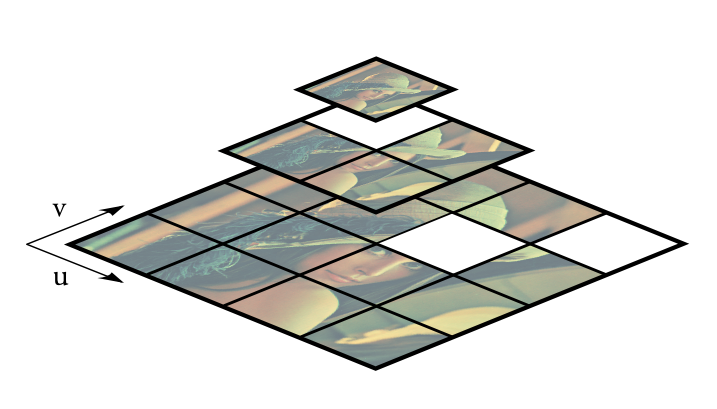
\includegraphics[width=0.6\textwidth]{images/megatextures-pyramid} }
				\subfloat[La texture virtuelle, composée de tiles de la pyramide]{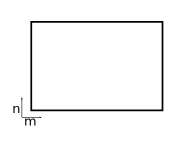
\includegraphics[width=0.4\textwidth]{images/megatextures-virtual} }
				\caption{Mégatexture}
				\label{fig:editmegatex}
			\end{figure}
		L'image est représentée par deux structures différentes, l'une se trouvant sur le disque et l'autre en mémoire.
		Celle qui se trouve sur le disque est la plus volumineuse des deux. Elle est composée d'une pyramide creuse de tiles. 

		Cette structure consiste en l'image gigapixel complète, divisée en tiles, les régions vides ou facultatives de l'image étant représentées par une absence
		de tiles, afin d'économiser de la mémoire. La structure contient aussi tous les mipmaps de cette image sous forme de tiles de dimensions identiques.

		En mémoire se trouve une texture, appelée \emph{texture virtuelle} qui a la taille maximum supportée par le matériel d'accélération, 
		ce qui est beaucoup moins que l'image originale. Cette texture est composée de tiles se trouvant dans la pyramide.
		
		\subsubsection{Affichage de l'image}
			Pour afficher une texture sur un maillage 3D, on assigne à chaque vertice  du maillage une coordonnée $u,v$ correspondant à un pixel de cette texture.
			de la texture. Comme nous désirons afficher la texture gigapixel, ces coordonnées correspondent aux pixels de cette texture.
			Celle-ci est cependant trop grande pour pouvoir être utilisée telle quelle.
			
			Pour résoudre ce problème on place les tiles qui nous intéressent dans une texture virtuelle qui est suffisamment petite pour pouvoir
			être utilisée pour l'affichage. Un \emph{pixel shader} est ensuite utilisé pour traduire lors de l'affichage les coordonnées $u,v$ de la
			texture gigapixel en les coordonnées $m,n$ de la texture virtuelle. 

			Pour déterminer quels tiles nous intéressent, on s'aide d'un premier rendu dans lequel on examine quelles régions de la texture gigapixel
			sont affichées, et à quelle résolution. On sélectionne ensuite les tiles qui couvrent cette zone avec la résolution la plus proche de celle
			affichée. Comme la résolution de l'écran est plus petite que celle de la taille de la texture virtuelle, on disposera toujours d'une place
			suffisante pour couvrir la quantité de texture affichée.

			Récupérer les tiles sur le disque implique un délai non négligeable. Le megatexturing incorpore des techniques permettant de pallier à
			ce problème qui sortent du cadre de cette présentation.

		\subsubsection{Édition de l'image}
			Pour générer et éditer l'image gigapixel, on utilise la technique précédente pour l'affichage, et on utilise les techniques de framework 
			bitmap pour appliquer les opérations; Celles-ci sont directement rasterisées dans la pyramide de tiles.
		\subsubsection{État de l'art du Mégatexturing}
			Le Mégatexturing à été popularisé par id Software pour son utilisation dans le moteur de jeu idTech4 et idTech5\cite{megatex1}\cite{megatex2}. Cette technique est utilisé
			par les jeux utilisant ces moteurs. D'autres moteurs tels que Torque ont réimplémenté cette technique.

	\section{Comparaison des différents framework}

	\begin{table*}
		\begin{tabular*}{\textwidth}{@{\extracolsep{\fill}} | l || c | c | c | c |}
			\hline
			Fonctionnalité	 		& Bitmap 		& Nodal 		& Vectoriel 		& Himalaya 	\\
			\hline \hline	                                                                                                          
			Dessin de primitives	   	& $\medbullet$		& $\ominus$		& $\medbullet$	 	& $\medbullet$	\\
			Peinture		   	& $\medbullet$		& $\ocircle$		& $\ominus$		& $\medbullet$	\\
			Filtres	colorimétriques	   	& $\medbullet$		& $\medbullet$		& $\ominus$		& $\medbullet$	\\
			Filtres	spatiaux	   	& $\medbullet$		& $\medbullet$		& $\ominus$		& $\ocircle$	\\
			Transformations vectorielles   	& $\ocircle$		& $\ocircle$		& $\medbullet$	 	& $\ocircle$	\\
			Transformations bitmap   	& $\medbullet$		& $\medbullet$		& $\ominus$	 	& $\ominus$	\\
			Modes de fusion		   	& $\medbullet$		& $\medbullet$		& $\medbullet$	 	& $\medbullet$	\\
			Modèles colorimétriques	   	& $\ominus$		& $\medbullet$		& $\ominus$	 	& $\medbullet$	\\
			Ton direct		   	& $\ominus$		& $\ocircle$		& $\medbullet$	 	& $\ocircle$	\\
			Modèles étendus		   	& $\ocircle$		& $\medbullet$		& $\ocircle$	 	& $\ominus$	\\
			Undo/Redo		   	& $\medbullet$		& $\ominus$		& $\medbullet$	 	& $\medbullet$	\\
			Édition non destructive	   	& $\ocircle$		& $\medbullet$		& $\medbullet$	 	& $\medbullet$	\\
			Composition non linéaire	& $\ocircle$		& $\medbullet$		& $\ocircle$	 	& $\medbullet$	\\
			Édition par pixel		& $\medbullet$		& $\ocircle$		& $\ocircle$	 	& $\ominus$	\\
			Indépendance à la résolution	& $\ocircle$		& $\ominus$		& $\medbullet$	 	& $\ocircle$	\\
			Images Gigapixel		& $\ocircle$		& $\medbullet$		& $\medbullet$	 	& $\medbullet$	\\
			Traitement d'images multiples	& $\ominus$		& $\medbullet$		& $\ocircle$	 	& $\ominus$	\\
			\hline
			\multicolumn{5}{|l|}{ \tiny $\medbullet$ : Fonctionnalité adaptée au framework.} \\
			\multicolumn{5}{|l|}{ \tiny $\ominus$ : Fonctionnalité implémentable dans le framework, mais de manière limitée ou peu performante.} \\ 
			\multicolumn{5}{|l|}{ \tiny $\ocircle$ : Fonctionnalité inadaptée au framework.}	\\
			\hline
		\end{tabular*}
		\caption{Grille de comparaison des fonctionnalités. }
		\label{comparaison}
	\end{table*}

	Le tableau~\ref{comparaison}, (page~\pageref{comparaison}) permet d'avoir une vision globale des fonctionnalités supportées par les différents 
	types de framework. On remarque que les frameworks proposent des fonctionnalités très différentes, ce qui explique pourquoi chaque 
	domaine d'application tend à préférer un framework en particulier.

	Ce tableau permet aussi de comparer les frameworks existants aux fonctionnalités adaptées au framework Himalaya qui est présenté dans ce mémoire. Cette
	comparaison reste en partie théorique puisque toutes ces fonctionnalités n'ont pas été implémentées et soumises à des tests utilisateurs. 
	
	Néanmoins ce framework propose une combinaison intéressante de fonctionnalité en combinant Peinture, Dessin de primitives, Édition non destructive, 
	Composition non linéaire et Images gigapixel. Non repris dans ce tableau est la possibilité -- encore théorique -- de pouvoir utiliser la technique
	de mégatexture en combinaison avec \emph{Himalaya} afin de permettre l'édition non destructive des textures d'une scène 3D temps réel.

	La suite de ce mémoire se concentrera sur la présentation de l'architecture et des fonctionnalités de base du framework Himalaya, pour se concentrer
	ensuite sur l'implémentation et l'évaluation par test utilisateurs des fonctionnalités de peinture et d'édition d'images gigapixel, combinaison de
	fonctionnalité n'étant proposée par aucun des frameworks existants.


	\chapter{Framework Himalaya (20 pages) }
	Himalaya est un framework d'édition d'image s'inspirant des frameworks nodaux et de la technique de megatextures. Il fut conçu par moi même avant la
	réalisation de ce mémoire dans le but de créer un logiciel de peinture permettant l'édition non destructive, la composition non linéaire, et d'être
	compatible avec la technique de mégatexture afin de pouvoir être utilisé dans le jeu vidéo. 


	\section{Structures de données}
		Nous allons présenter ici les structures de données de base du framework. S'il est souvent difficile de justifier la conception de ces structures
		sans examiner les algorithmes qui les utilisent, il est encore plus difficile de comprendre les algorithmes sans connaitre ces structures.
		Nous avons donc fait le choix de présenter et d'expliquer tant que possible ces structures, le reste sera présenté à la section suivante qui
		vous parlera des différents algorithmes.

		Les structures et les algorithmes seront également présentés dans le langage \emph{C}, plutôt que dans des formes plus abstraites. Ceci afin de nous
		rapprocher de l'implémentation --- également réalisée en \emph{C} --- et donc de pouvoir plus facilement discuter des performances de celle-ci. 
		Il faut toutefois noter que les structures telles que présentées dans ce rapport sont plus simples que celles de l'implémentation. En effet, 
		la gestion des modèles colorimétriques est ommise, de même que des extensions propres à l'implémentation, pour permettre par exemple une
		déboguage plus facile, et l'introspection sur les données. 

		\subsection{Les Tiles}
		Comme dans bien d'autres framework, les images d'himalaya sont divisés en grilles de tiles. Un tile est donc un bitmap rectangulaire correspondant
		à une petite région de l'image. Himalaya fait un plus grand usage des tiles que d'autres frameworks puisque toute opération prend des tiles
		en entrée et en sortie. Un tile représente donc la plus petite unité de traitement, et un intérèt particulier doit être apporté à sa conception.

		\subsubsection{Structure du tile}
			Il y a trois caractéristiques importantes à prendre en compte lorsque l'on conçoit un tile:
			\begin{description}
				\item[Sa taille en mémoire]Un premier intérèt des tiles est qu'ils sont une unité de mémoire pouvant être suffisemment petite
				pour tenir intégralement dans les caches du processeur et ainsi éviter des accès cache invalides fort coûteux en temps de calcul.
				Les processeurs de différent modèles ont différentes taille de cache et différentes manières de les gérer. Plus le tile est petit,
				plus il sera rapide de les traiter sur une grande gamme de processeurs.
				
				Cependant, si le tile est trop petit, les gains réalisés par sa taille sont perdu par la surcharge de travail que doit faire le
				framework pour gérer ces tiles. 

				En outre, si tous les tiles ont la même taille en mémoire, on réduit les risques de fragmentation, et on peut faire des
				allocateurs optimisés qui allouent les tiles de manière contigue et réutilisent les tiles libérés.

				\item[Sa taille en pixel] Si tous les pixels ont la même taille en pixel, alors les images de dimensions égales seront
				toujours divisées en tiles de la même manière, ce qui rend plus simples beaucoup d'algorithmes du framework.
				la programmation des opérations en sera également facilitée. 

				Cependant, un framework moderne doit prendre en compte la gestion de modèles colorimétriques, et niveaux de quantification
				différents. La représentation d'un pixel peut donc avoir des empreintes mémoire différentes, il faudra donc choisir entre
				avoir des tiles de même taille pixel, ou des tiles de même taille mémoire.

			\begin{figure}[h]
				\centering
				\subfloat[Un tile normal]{ \label{fig:render} 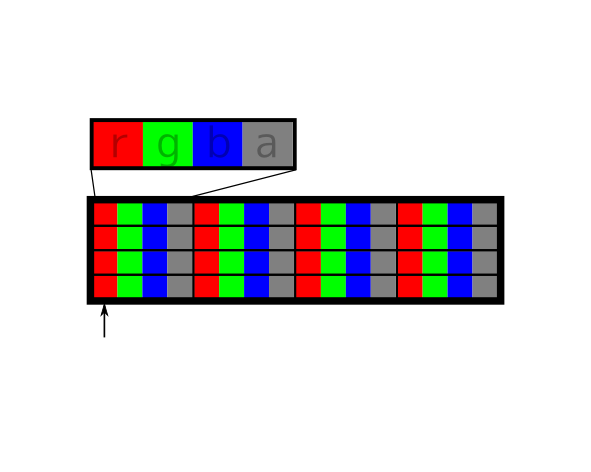
\includegraphics[width=0.5\textwidth]{images/tile-a} }
				\subfloat[Un tile aux canaux séparés]{ \label{fig:render-hsv} 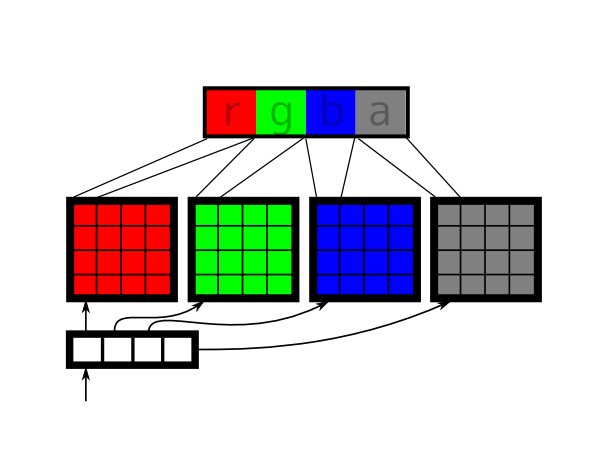
\includegraphics[width=0.5\textwidth]{images/tile-b} }
				\caption{Deux structures de tiles}
				\label{fig:tilestruct}
			\end{figure}
				\item[La répartition des pixels dans le tile] La manière commune de représenter un pixel au sein d'un bitmap est d'avoir
				toutes ses composantes placées dans des emplacement contigus. Une autre manière est de placer chaque composante dans un
				bitmap séparé. Un tile étant alors constitué de plusieurs bitmaps. L'intéret de cette technique est que les tiles de même
				quantisation ont la même taille en pixel, et les bitmaps les constituant la même taille en mémoire. Un autre intérèt est
				qu'il est maintenant beaucoup plus facile de programmer des opérations qui peuvent gérer un nombre quelconque de composantes
				par pixel.

				Cependant, cela implique que l'accès à un pixel nécessite autant d'accès mémoires que de composantes, ce qui ralentit 
				l'exécution du programme. 
			\end{description}

		\subsubsection{Comparaison des tiles}
			Le tableau TODO représente le résultat d'expériences qui résument les concepts précedemment exposés. Dans ce tableau, deux opérations
			sont testées : \emph{colorfill} consiste à remplir une image de $8192^2$ pixels \emph{RGBA} 8bits/composante d'une couleur unie. \emph{blend} consiste 
			en fusionner deux images de $8192^2$ pixels \emph{RGBA} 8 bits/composante par opacité. Ces deux opérations 
			sont utilisées très couramment pour la réalisation de peintures. 

			Ces opérations sont appliquées selon des schémas différents: \emph{colorfill\_full} remplit tous les tiles de l'image, alors que \emph{colorfill\_single}
			remplit un tile choisit au hasard autant de fois qu'il y a de tiles dans l'image. Le même nombre de pixels est donc traité dans les deux tests,
			mais le second devra accéder régulièrement à de nouvelles zones mémoire.

			Même chose pour les operations \emph{blend} : \emph{blend\_full} fusionne les tiles des deux images, \emph{blend\_single} fusionne deux tiles
			sélectionnés au hasard, \emph{blend\_intermediate} fusionne toute l'image sur un seul tile. Ce dernier test est fort représentatif de la
			manière dont les tiles sont utilisés dans Himalaya.

			Ensuite les tiles normales sont comparées aux tiles à canaux séparés. 
			

			\begin{table*}
				\label{tileperf}
				\tiny
				\begin{tabular*}{\textwidth}{@{\extracolsep{\fill}} | r | c || c | c | c | c | c | c | c | c | c |}
					\hline
					\multicolumn{2}{|r||}{Largeur des tiles}& 8	& 16	& 32	& 64	& 128	& 256	& 512	& 1024	& 2048	\\
					\hline 
					Test	& Tile &\multicolumn{9}{ c|}{Temps de calcul moyen sur 5 expériences (secondes)}\\
					\hline
					\emph{colorfill\_single} & Normal 	& 0.78	& 0.64 	& 0.58	& 0.57	& 0.49	& 0.28	& 0.28	& 0.28	& 0.31	\\
					\emph{colorfill\_full} & Normal 	& 1.14	& 0.7 	& 0.65	& 0.63	& 0.55	& 0.44	& 0.47	& 0.44	& 0.51	\\
					\emph{colorfill\_single}& Séparé 	& 1.30	& 1.06 	& 1.04	& 1.06	& 0.97	& 0.79	& 0.79	& 0.79	& 0.80	\\
					\emph{colorfill\_full} & Séparé 	& 2.14	& 1.39 	& 1.16	& 1.12	& 1.10	& 1.03	& 1.00	& 1.01 & 1.01	\\
					\hline\hline
					\emph{blend\_single} & Normal 		& -	& 3.12 	& 2.98	& 3.0	& 3.08	& 4.16	& 13.58	& 19.97	& 22.60	\\
					\emph{blend\_inter} & Normal 		& -	& 5.31 	& 5.20	& 4.96	& 5.12	& 4.85	& 13.49	& 20.46	& 20.64	\\
					\emph{blend\_full} & Normal 		& -	& 5.39 	& 5.19	& 5.17	& 5.0	& 5.42	& 13.15	& 20.44	& 21.12	\\
					\emph{blend\_single}& Séparé		& -	& 6.29 	& 5.64	& 5.39	& 6.61	& 6.50	& 18.67	& 27.48	& 28.92	\\
					\emph{blend\_inter}& Séparé		& -	& 6.55 	& 5.69	& 5.50	& 6.55	& 6.74	& 20.22	& 27.77	& 27.48	\\
					\emph{blend\_full} & Séparé	 	& -	& 6.68 	& 5.82	& 5.45	& 6.59	& 6.78	& 18.39	& 27.41 & 27.23	\\
					\hline
				\end{tabular*}
			\end{table*}
			\begin{figure}[h]
				\centering
				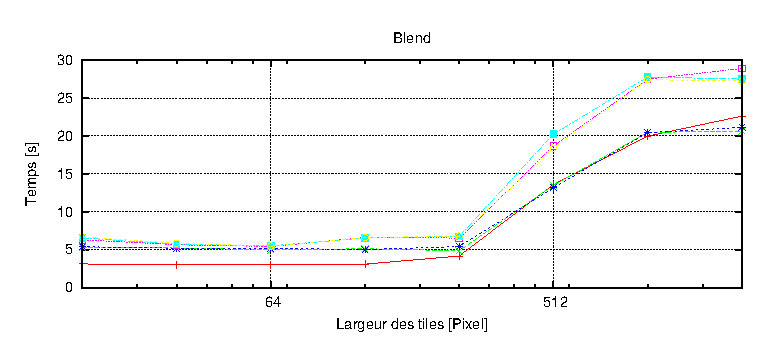
\includegraphics[width=\textwidth]{images/tilegraph.eps} 
				\label{fig:tilegraph}
			\end{figure}
		\subsubsection{Analyse des performances}
			On peut tirer plusieurs conclusion de ces expériences:
			\begin{itemize}
				\item Les tiles doivent être les plus grands possibles, pour diminuer le 
			nombre d'appels de fonctions, mais ne doivent pas être trop grands, sinon les performances sont très fortement dégradées. 
				\item Les tiles à canaux séparés sont jusque 2 fois plus lents que les tiles normaux.
				\item Le schémà d'accès aux tiles en mémoire a un impact non négligable mais plus marqué sur les tiles normaux.
				\item Le temps pour faire la fusion d'un même nombre de pixels peut différer de 970\% selon le type de tile, sa taille et la
				manière dont il est utilisé, puisque cette opération représente la grande majorité du temps de calcul du framework, ce choix
				est particulièrement important.
			\end{itemize}
			Enfin, il ne faut pas oublier que ces expériences ommettent deux facteurs importants: Le fait que la gestion des tiles dans le framework 
			est bien plus lourde, ce qui favorise les tiles plus grands, et le fait que les tiles plus petits permettent plus de précision dans 
			la localisation des opérations, ce qui permet de réduire le nombre de pixels accédés à chaque opération.

			Déterminer l'importance de ces deux facteurs requiert d'avoir des données d'utilisation du framework représentatives, par exemple
			avec des tests utilisateur. 
		\subsubsection{Structure finale}
			Le choix s'est porté sur des tiles normaux de taille fixe de $32\times32$ pixels, et ce quelque soit le modèle colorimétrique utilisé.

		\subsection{Les Frames}
			La Frame est la structure de donnée qui organise les tiles. Elle doit remplir plusieurs fonctions: stocker une image gigapixel,
			stocker les mipmaps de cette image, et servir de cache aux résultats des opérations, ainsi que les mipmaps de ceux-ci.

			L'intérèt des mipmaps est que pour un coût mémoire de seulement 33\% de l'image originale, ils permettent d'accéder à une sous région
			de l'image à une échelle quelconque en un temps ne dépendant que de la taille de cette sous-région, et non de la taille de l'image. 
			Cette propriété est indispensable pour pouvoir travailler sur des images giga-pixel.
			
			La Frame est une pyramide de tile creuses. Cette structure n'est pas nouvelle et est utilisée dans la pluspart des logiciels devant
			gérer des images gigapixel et leurs mipmaps. Les formats d'échange standard des photos satellites sont par exemple basés sur ces structures.
			
			L'intérèt d'avoir une pyramide creuse est de pouvoir stocker des tiles individuels, ce qui est indispensable pour pouvoir s'en servir
			comme d'une cache.

			Il existe plusieurs structures permettant l'organisation de tiles en pyramide creuses. La plus populaire est le quadtree, et c'est celle
			qui fut choisie pour l'implémentation des Frames.

			\subsubsection{Les quadtrees}
		\begin{lstlisting}[float,caption={Définition des hlFrameNodes},frame=tb,label=lsthlFrameNode]
typedef struct hl_frame_node{
	/* abscisse du tile */
	int tx;
	/* ordonnee du tile */
	int ty;
	/* tile  */
	hlTile *tile;
	/* Noeuds enfants */
	hlFrameNode *tl;
	hlFrameNode *tr;
	hlFrameNode *bl;
	hlFrameNode *br;
}hlFrameNode;
		\end{lstlisting}
				Les quadtrees sont composés de noeudsayant chacun une référence optionelle vers un tile, et de quatre références vers
				les noeuds enfants. 

				Chaque ensemble de noeuds de la même profondeur représente ainsi un bitmap à l'échelle deux fois plus petite que l'ensemble de
				noeuds à la profondeur suivante.

				Une définition de la structure des noeuds se trouve au listing~\ref{lsthlFrameNode}, page~\pageref{lsthlFrameNode}

			\subsubsection{Placer une image dans le Quad-Tree}
				Afin d'éviter d'avoir des Quad-Trees inutilement profond, les images sont stoquées au niveau le moins profond pouvant les contenir,
				soit $ceil( \log_2( max(size_x,size_y)/32))$, $size_x$,$size_y$ représentant la largeur et la hauteur de l'image en pixels.
				Cette profondeur est ensuite stoquée dans la Frame afin de pouvoir identifier le niveau correspondant à la résolution native.

			\subsubsection{Référencer les Tiles dans le Quad-Tree}
				Les tiles sont référencés par trois coordonnées $(t_x,t_y,t_z)$. $t_x,t_y$ représente les coordonnées spatiales du tile, $t_x$ valant
				zéro à l'extrémité gauche du bitmap, et étant positif à droite. $t_y$ vaut zéro à l'extrémité supérieure du bitmap et est positif vers le bas,
				et ce quelque soit l'échelle représentée.
				
				$t_z$ représente le niveau d'échelle. Il représente habituellement la profondeur du noeud à laquelle on trouve le tile. Nous avons
				choisi d'utiliser un système différent, $t_z$ vallant $0$ au niveau correspondant à la résolution native, et étant positif
				pour les échelles intérieures. L'intérèt de ce système est que la référence d'un tile est indépendante de sa profondeur réelle,
				qui peut changer lorsque l'on insère ou retire des tiles dans celui-ci.
				
				On peut s'intéresser à la valeur maximale de $t_z$ qui dépend de la taille de l'image stockée dans le quadTree.
				Comme nous voulons pouvoir indexer les pixels indépendemment, la largeur de l'image ne peut dépasser
				\emph{MAX\_INT}, Ce qui correspond à une valeur maximale de $t_z$ de $26$ sur les architectures 32bits, avec des tiles de 32 pixels
				de coté.
				
			\subsubsection{Les coordonnées négatives}
				Lorsque la Frame sert à stocker un bitmap chargé depuis le disque, les pixels le constituant, et donc les tiles, ont toujours des
				coordonnées $t_x,t_y$ positives. Cependant, il est pratique de pouvoir également stocker des pixels de coordonnées négatives, afin
				de disposer du plan complet pour pouvoir stocker le résultat de transformations géométriques. Pour ce faire, la Frame
				stoque un Quad-Tree par quadrant, et les tiles aux coordonnées négatives sont redirigées vers les Quad-Tree correspondant.

			\subsubsection{Le Tile de fond}
				Lorsque la frame est utilisée pour contenir un bitmap, celle-ci dispose d'un Tile de fond. Celui-ci n'est pas repris
				dans les Quad-Tree et est d'une couleur unie correspondant au 'fond' de l'image, habituellement une couleur transparente.
				Lorsque l'on tente d'accéder à une coordonnée qui ne correspond à aucun noeud des Quad-Trees, ce que l'on a atteint une zone
				correspondant au fond de l'image, et le tile de fond est renvoyé. Ceci permet de réduire l'espace mémoire consommé par les zones 
				vides des images.

			\subsubsection{Insertion, suppression et accès aux tiles}
				L'insertion, la suppression, et l'accès à un tile se fait en $O(n)$ ou $n$ est la profondeur à laquelle se trouve le tile dans 
				le Quad-Tree. Comme $n$ ne dépasse pas 26, le temps d'exécution de ces fonctions est borné, et on peut donc considérer que'elles
				ont une complexité de $O(1)$. 
				
				De plus l'insertion et la suppression augmentent ou diminuent automatiquement la taille des 
				quad-tree afin de s'assurer que la taille de l'arbre reste minimale. Ceci nécessite cependant de stocker à chaque noeud 
				sa coordonnée $t_x,t_y$, ce qui augmente leur taille de 40\%. TODO / evaluer l'espace pris.

			\subsubsection{Surchage mémoire}
				Les FrameNode ont un poids de $28$ Bytes, ce qui représente 2,66\% de la taille des tiles les plus petits(Alpha 8bit), 0.67\% de celle des plus
				communs(RGBA 8bit)  et 0.14\% de celle des plus grands(CMYKA 32bit). Dans le meilleur des cas, le stockage d'un tile ne 
				nécessite qu'un noeud, et 26 dans le pire des cas. On observe lors des tests utilisateurs qu'en moyenne le stockage d'un tile
				nécessite TODO noeuds, ce qui représente TODO pourcent.
			\subsubsection{Définition de l'hlFrame}
		\begin{lstlisting}[float,caption={Définition des hlFrames },frame=tb,label=lsthlFrame]
typedef struct hl_frame{
	/* largeur en pixel du bitmap */
	int sizex;
	/* hauteur en pixel du bitmap */
	int sizey;
	/* tile de fond */
	hlTile *bg;
	/* QuadTrees */
	hlFrameNode *tl;
	hlFrameNode *tr;
	hlFrameNode *bl;
	hlFrameNode *br;
}hlFrame;
		\end{lstlisting}
		\begin{lstlisting}[float,caption={API Publique des hlFrame},frame=tb,label=lsthlFrameAPI]
/* Place un tile dans f aux coordonnees tx,ty,tz */
void	hlFrameTileSet(hlFrame *f, hlTile *t, int tx, int ty, int tz); 
/* Enleve et renvoie le tile tx,ty,tz de f */
hlTile *hlFrameTileRem(hlFrame *f, int tx, int ty, int tz); 
/* Renvoie le tile tx,ty,tz, si il existe, NULL sinon. */
hlTile *hlFrameTileGet(const hlFrame *f, int tx, int ty, int tz);
/* Renvoie le tile tx,ty,yz si il existe, le tile BG sinon. */
hlTile *hlFrameTileRead(const hlFrame *f, int tx, int ty, int tz);
		\end{lstlisting}
				On trouve au Listing~\ref{lsthlFrame}, page~\ref{lsthlFrame} une définition de la structure des hlFrame.
				On trouvera également au Listing~\ref{lsthlFrameAPI}, page~\ref{lsthlFrameAPI}, 
				l'API publique des hlFrame.


		\subsection{L'hlImage}
		\begin{lstlisting}[float,caption={Définition des hlImages },frame=tb,label=lsthlImage]
typedef struct hl_image{
	/* Reference vers la derniere operation de la pile*/
	hlOperation *top;
	/* Reference vers la frame contenant le bitmap 
	 * a modifier */
	hlFrame *source;
}hlImage;
		\end{lstlisting}
		\begin{figure}[h]
			\centering
			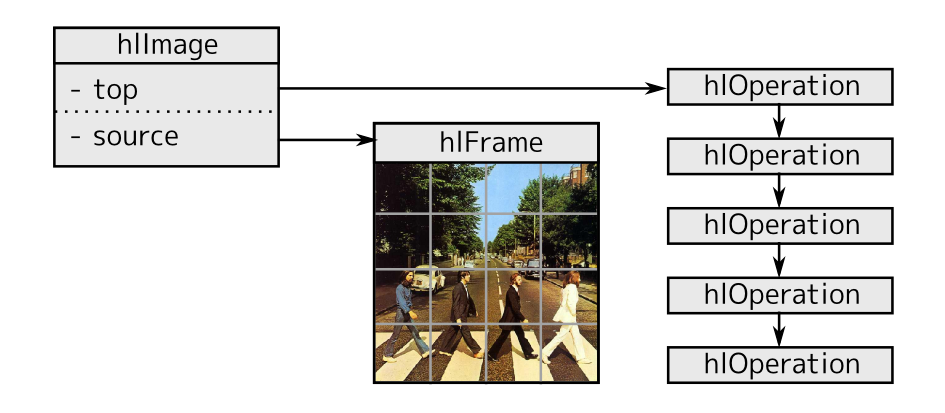
\includegraphics[width=\textwidth]{images/hlImage1} 
			\label{fig:hlImage1}
			\caption{une hlImage, avec la source et la pile d'opération}
		\end{figure}
		Si la frame représente une cache ou un bitmap, l'hlImage représente une image à proprement parler. L'hlImage est composée principalement
		de deux choses, une Frame représentant la source, c'est à dire une image de départ à modifier, et une pile d'opérations
		qui modifient l'image.	
		Une défintion de la structure se trouve au Listing~\ref{lsthlImage}, page~\pageref{lsthlImage} 

		\subsubsection{La pile d'opérations}
		\begin{lstlisting}[float,caption={API des hlImages },frame=tb,label=lsthlImageAPI]
/* Rasterise un tile de l'image */
hlTile *hlImageRenderTile(hlImage *img, int tx, int ty, int tz);
/* Insere une operation au sommet de la pile */
void hlImagePushOp(hlImage *img, hlOperation *op);
/* Enleve une operation du sommet de la pile */
hlOperation *hlImagePopOp(hlImage *img);
/* Enleve une operation de la pile et la renvoie */
hlOperation *hlImageRemOp(hlImage *img, int index);
/* Insere l'operation dans la pile */
void hlImageInsertOp(hlImage *img, hlOperation *op, int index);
/* Renvoie l'indice auquel se trouve l'operation d'uid opUid */
int hlImageOpIndex(hlImage *img, int opUid);
		\end{lstlisting}
			La pile d'opération représente l'ensemble des opérations qui vont modifier l'image source pour obtenir l'image dessinée, les opérations
			du bas de la pile s'appliqaunt en premier. Il est
			possible de manipuler cette pile par l'API publique de l'hlImage. Les opérations les plus communes sont l'ajout et le retrait d'opération
			au dessus de la pile, l'insertion et la suppression d'opérations se trouvant au  milieu. Cette API est résumée dans le 
			listing~\ref{lsthlImageAPI}, page~\pageref{lsthlImageAPI}


			Les opérations se trouvant à l'intérieur de la pile peuvent être accédées par leur indice de position dans la pile, mais aussi leur
			$uid$, identifiant propre à chaque opération. 

			La pile d'opération est implémentée par une liste simplement chainée. Chaque opération référence l'opération \emph{précédente}.
			L'\emph{hlImage} référence uniquement la \emph{dernière} opération. Les raisons de cet ordre apparaitront clairement à la vue
			de l'algorithme de rasterisation.

		\subsection{Les hlOperations}
		\begin{lstlisting}[float,caption={Définition des hlOperations },frame=tb,label=lsthlOp]
typedef struct hl_operation{
	/* Reference vers la classe de l'operation */
	hlOpClass  *class;	
	/* Reference vers l'operation precedente. */
	struct hl_operation *down;
	/* Frame qui sert de cache aux resultats de 
	 * l'operation */
	hlFrame *cache;			
	/* Reference vers l'image a laquelle appartient 
	 * l'operation */
	hlImage *image;			
	/* HL_MODIFABLE, HL_CACHING */
	int	 flags;			
	/* Un compteur de references */
	int	 refcount;		
	/* Un identifiant unique a l'operation*/
	int 	uid;
	/* Les parametres de l'operation */
	void	*params;		
}hlOperation;
		\end{lstlisting}

		Les hlOperations sont les objets qui représentent toutes les opérations qui permettent de modifier une image. Une définition de la structure
		se trouve au Listing~\ref{lsthlOp}, page~\pageref{lsthlOp}. Certaines opérations particulières pouvant étendre cette structure avec des
		champs supplémentaires, qui seront détaillés dans les sections appropriées.

		Cela représente un minimum de 32Bytes\footnote{La structure telle qu'implémentée possède de nombreux champs supplémentaires à de fins de déboguage et fait
		92Bytes} par opération sur une architecture 32bits. Une hlOperation est donc suffisemment légère pour
		que l'on puisse en utiliser plusieurs millions sans problèmes de mémoire. 

		\subsubsection{La classe d'opération}
			\begin{lstlisting}[float,caption={Définition des classes d'opérations },frame=tb,label=lsthlOpClass]
typedef struct hl_op_class{
	/* HL_COLORFILTER, HL_FILTER, HL_DRAW, HL_BLEND */
	int category;
	/* Numero de l'operation*/
	int id;
	/* le nombre de parametres flottants */
	int float_param_count;
	/* le nombre de parametres entiers */
	int int_param_count;
	/* le nombre de parametres de couleur */
	int color_param_count;
	/* le nombre de parametres d'images */
	int image_param_count;
}hlOpClass;
			\end{lstlisting}
			La classe d'opération contient la description d'un type d'opération, et tout ce qui est commun à ces opérations, Il n'existe qu'une
			seule instance de chaque classe d'opération. La définition de ces classe est donnée au listint~\ref{lsthlOpClass}, page~\pageref{lsthlOpClass}.

			Les champs des classes d'opérations méritent d'être expliqués plus en détails	
			\begin{description}
				\item[\texttt{category}]. Les opérations sont divisées en plusieurs catégories, selon les propriétés et les paramètres
				nécessaires à l'application de l'opération. Ceci permettra d'appeler une méthode spécialisée pour chaque catégorie d'opération.
				Ces catégories correspondent également aux différentes catégories d'opération de dessin que nous avons vu au premier chapitre. 
				\begin{description}
					\item[\texttt{HL\_COLORFILTER}]: Les filtres colorimétriques. Ces filtres ne sont pas dépendants de la position du tile ou de son échelle, et s'appliquent
					sur toute l'image. 
					\item[\texttt{HL\_FILTER}]: Les filtres spatiaux. Ces filtres dépendent de l'échelle, de la position du tile, 
					et ne peuvent modifier un tile sans connaitre les données des tiles adjascents.
					\item[\texttt{HL\_DRAW}]: Le dessin de primitives. Ces opérations dépendent de l'échelle et de la position du tile, 
					mais ne s'appliquent que sur une sous-région de l'image.
					 Ces filtres dépendent de l'échelle et de la position du tile, et ne s'appliquent que sur
					une sous région de l'image.
					\item[\texttt{HL\_BLEND}]] Les opéartions de fusion. Ces opérations dépendent de la position du tile et de son échelle, 
					ainsi que d'une autre \emph{hlImage}
					\item[\texttt{HL\_COLORMODEL}]] Les opérations pour lesquelles les tiles en entrée n'ont pas le même modèle colorimétrique
					qu'en sortie. 
				\end{description}
				\item[\texttt{id}]Le numéro de l'opération, qui l'identifie dans sa catégorie. Par exemple, Le dessin de cercle 
				--- \texttt{HL\_DRAW\_CIRCLE} --- dans 
				la catégorie \texttt{HL\_DRAW}
				\item[\texttt{*\_param\_count}]: Le nombre de paramètres de chaque type. Les opérations sont limitées à quatre types de paramètres,
				les flottants, les entiers, les couleurs, et les images. Cette information est nécessaire pour pouvoir calculer la taille des 
				paramètres de la fonction. L'implémentation utilise un mécanisme similaire mais plus complexe permettant une introspection sur les
				paramètres.
			\end{description}
	\section{Algorithmes}
		\subsection{Dessin}
		Dans Himalaya, le dessin et la rasterisation sont deux opérations séparées et indépendantes. Le dessin consiste simplement à ajouter une 
		opération au dessus de la pile.

		\subsection{Rasterisation}
		L'algorithme de rasterisation d'himalaya s'inspire de l'algorithme de rasterisation des frameworks nodaux, et du raytracing.
		Là ou les algorithmes de rasterisation des frameworks bitmaps et vectoriels appellent les opérations dans l'ordre avec lequel
		elles ont été ajoutées, himalaya les appelles dans l'ordre inverse; depuis la dernière jusqu'à la première.  En outre, comme dans
		le raytracing, l'algorithme de rasterisation d'himalaya peut se faire indépendemment pour chaque pixel, et donc pour chaque tile. 

		Ceci a plusieurs intérèts :
		\begin{itemize}
			\item Si une opération a son résultat en cache, on peut réutiliser ce résultat sans examiner les opérations antérieures.
			\item Si une opération est opaque, c'est à dire qu'elle masque le résultat des opérations précédentes, on peut l'appliquer
			sans examiner les opérations entérieures.
			\item Si la rasterisation d'un tile est indépendant de celui de son voisin on peut utiliser un thread par calcul de tile, et donc
			exploiter facilement le multi-thread.
			\item Si la rasterisation d'un tile est indépendant de celui de son voisin, on peut identifier les tiles de la région à visualier,
			et ne rasteriser que ceux-ci. Le temps de rendu est donc proportionnel à la région à visualiser, et non à la taille de l'image sur
			laquelle on travaille. Cette propriété est indispensable pour travailler sur des images gigapixel.
		\end{itemize}

		\begin{lstlisting}[float,caption={Rasterisation d'opérations},frame=tb,label=lsthlOpRenderTile]
hlTile *hlOpRenderTile(hlOperation *op, int tx, int ty, int tz){
	hlTile *tile = hlFrameTileGet(op->cache,tx,ty,yz);
	if(tile){
		if(hlOpCaching(op,tx,ty,yz)){
			return hlTileCopy(tile);
		}else{
			return hlFrameTileRem(op->cache,tx,ty,yz);
		}
	}else{
		if(hlOpOpaque(op,tx,ty,yz)){
			tile = hlTileNew();
			hlOpRasterise(tile,op,tx,ty,yz);
		}else{
			if(op->down){
				tile = hlOpRenderTile(
				  op->down,tx,ty,yz);
			}else{
				tile = hlTileCopy(hlFrameTileGet(
				  op->image->source,tx,ty,tz));
			}
			hlOpRasterise(tile,op,tx,ty,yz);
		}
		if(hlOpCaching(op,tx,ty,tz)){
			hlFrameTileSet(	op->cache,
				hlTileCopy(tile),tx,ty,yz);
		}
		return tile;
	}
}
hlTile *hlImageRenderTile(hlImage *img, int tx, int ty, int tz){
	if(img->top){
		return hlOpRenderTile(img->top,tx,ty,tz);
	}
	return NULL;
}
	\end{lstlisting}
		Le listing~\ref{lsthlOpRenderTile}, page~\pageref{lsthlOpRenderTile} Montre une version simplifiée de l'algorithme
		de rasterisation. Examinons le en détail :
		\paragraph{Spécification:}
		\begin{description}
			\item[pre] --
			\item[tx, ty, yz] sont les coordonnées du tile à rasteriser. Ces coordonnées correspondent aux tiles du résultat,
			et non à celles de la Frame source.
			\item[op] est l'opération que l'on désire rasteriser.
			\item[returns] l'algorithme renvoie un nouveau tile qui est le résultat de toutes les opérations de l'image antérieures
			et égales à op, appliquées sur les données de la Frame source. Il faut libérer ce tile après utilisation.
			\item[post] Le résultat de cette opération est mis dans la cache de celle-ci.
		\end{description}
		
		\paragraph{Analyse ligne par ligne}
		\begin{description}
			\item[2.] La première chose à faire est de récupérer le résultat de l'opération dans la cache. 
			\item[3-8.] Si le résultat était dans la cache, on le renvoie
			\item[4-5.] Si l'opération doit encore garder ce tile en cache, on renvoie une copie.
			\item[6-7.] Sinon on l'enlève de la cache et on le renvoie.
			\item[9-27.] Le résultat n'étant pas dans la cache, il faut le calculer.
			\item[10-12.] On fait appel à l'opération pour savoir si son effet est opaque, et donc indépendant du résultat des opérations
			 précédentes. Si c'est le cas, on crée un tile vide (ligne 7) et on applique l'opération sur ce tile.
			\item[13-22.] L'opération n'est pas opaque, il faut donc l'appliquer sur le résultat des opérations précédentes.
			\item[14-16.] S'il y a une opération précédente on récupère son résultat par un appel récursif de cette fonction sur l'opération
			précédente.
			\item[17-19.] S'il n'y a pas d'opération précédente c'est que l'on est à la première opération, qui s'applique sur la Frame Source.
			\item[21.] \emph{tile} vaut désormais le résultat des opérations précédentes. On peut donc lui appliquer l'opération en cours.
			\item[23-25.] S'il est intéressant de mettre en cache à cette opération, on met une copie du tile en cache.
		\end{description}

		\lstinline$hlOpRenderTile(..)$ n'est cependant pas accessible à l'utilisateur, puisque celui ci n'a pas d'accès direct aux opérations de la pile.
		Pour rasteriser l'image il utilise \lstinline$hlImageRenderTile(..)$ 
		
		\subsubsection{Complexité spatiale et temporelle}
		La complexité temporelle de l'application d'une opération sur un tile est de $O(1)$ puisque les tiles possèdent un nombre fixe de pixel. 
		La complexité temporelle de l'insertion et du retrait dans la chache est également de $O(1)$. Chaque appel récursif à \lstinline$hlOpRenderTile(...)$
		Se fait donc en $O(1)$. La complexité temporelle de la rasterisation d'un tile est donc de $O(n)$ ou $n$ est le nombre 
		d'opérations ajoutées au sommet de la pile depuis la dernière rasterisation de ce tile. 

		Pour rasteriser une région, de l'image, il faut identifier les tiles correspondant à cette région, et les rasteriser un par un. La complexité
		temporelle pour rasteriser une région de l'image est donc de $O(m*n)$ ou $m$ est le nombre de tiles dans la région, et $n$ le nombre d'opérations
		ajoutées au sommet de la pile depuis le dernier rendu de cette région. 

		Cette complexité est particulièrement adaptée à la peinture, puisque très peu d'opération sont ajoutées sur la pile entre chaque rendu.
		Elle est également particulièrement adaptée à l'édition d'images gigapixel, puisque la taille de l'image n'intervient pas. 
		
		L'algorithme de rasterisation ne met en cache que lorsque l'opération le requiert, et enlève automatiquement les tiles des caches lorsque
		les opérations ne le requièrent plus. Cela garantit qu'aucun tile inutile ne reste en mémoire. La complexité spatiale dépend donc du
		nombre d'opérations qui requièrent de mettre en cache. Ceci sera détaille à la section \emph{Gestion de la cache}
		
		\subsubsection{Catégories d'opérations}
		L'algorithme tel que présenté n'est pas adapté à toutes les catégories d'opérations. Les filtres spatiaux nécessitent par exemple plusieurs tiles
		résultant de l'opération précédente pour en calculer un seul. Quand aux opérations de fusion, elles nécessitent d'obtenir le tile d'une
		autre image. Il faut donc un algorithme légèrement différent par catégorie. TODO.
		
	\section{États}
		La définition de l'hlImage telle que présentée jusqu'à maintenant n'est pas complète. En effet, comment modifier la pile d'opération sans
		corrompre les caches des opérations ? Comment défaire et refaire facilement des changements dans la pile ? 
		
		Pour permettre cela nous avons besoin d'introduire un mécanisme d'état. Un état est un \emph{uid} qui nous permet de sauvegarder et rétablir la
		pile d'opération et les paramètres de celle-ci. Ainsi il est possible de sauvegarder l'état de l'hlImage, d'ajouter, d'enlever, 
		de modifier des opérations, et de récupérer l'hlImage telle qu'elle état en chargeant l'état.

		Les états sont manipulés avec les fonctions suivantes :
		\paragraph{Fonction de manipulation d'États}
		\begin{itemize}
			\item \lstinline$hlState hlStateSave(hlImage *img)$ sauvegarde la pile d'opération dans un nouvel état. 
			\item \lstinline$hlState hlStateGet(hlImage *img, hlState s)$ renvoie l'état dans lequel se trouve l'image.
			\item \lstinline$void hlStateLoad(hlImage *img, hlState s)$ rétablit l'image à un état. 
			\item \lstinline$void hlStateRem(hlImage *img, hlState s)$ supprime un état de l'image. 
		\end{itemize}

		L'API publique de l'hlImage, combinée à l'API d'état est déjà suffisemment complète pour pouvoir réaliser  un logiciel de peinture. 
		
		\subsection{Implémentation des états}
			Les états sont des références vers des opérations de l'image. Ces références sont implémentées par une table de hachage qui
			associe à chaque état une opération. 

			Une fois qu'une opération est référencée par un état, elle ne peut plus être modifiée. Il en va de même pour toute opération
			antérieure à celle référencée, puisqu'une modification de celle-ci pourrait entrainer une modification du résultat de l'opération 
			référencée.

			Pour savoir si une opération est référencée --- directement ou indirectement --- par un état, chaque opération contient un
			compteur de référence qui compte le nombre d'états les référençant. 

		\begin{lstlisting}[float,caption={Définition des hlImages avec états },frame=tb,label=lsthlImage2]
typedef struct hl_image{
	/* Reference vers la derniere operation de la pile*/
	hlOperation *top;
	/* Reference vers la frame contenant le bitmap 
	 * a modifier */
	hlFrame *source;
	/* Hashtable associant les etats aux operations */
	HashTable *statelib;
	/* Etat en cours */
	hlState state;
}hlImage;
		\end{lstlisting}

		\begin{figure}[ht]
			\centering
			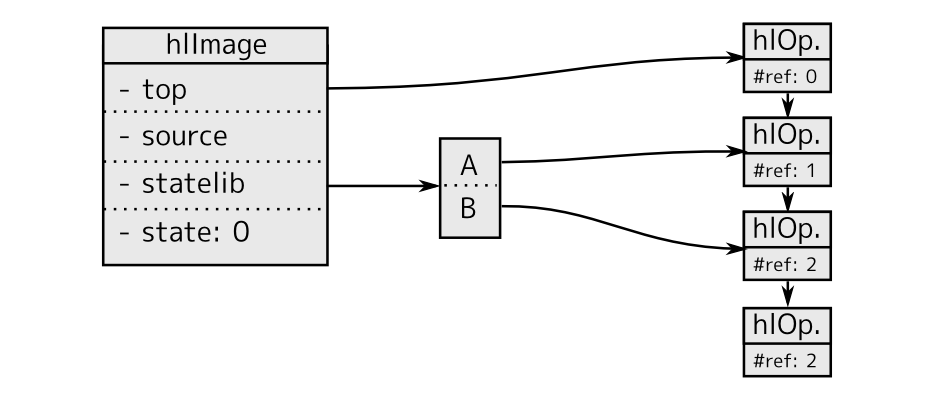
\includegraphics[width=\textwidth]{images/hlImage2} 
			\label{fig:hlImage2}
			\caption{une hlImage, avec une pile d'opérations et deux états}
		\end{figure}

			La structure de l'hlImage doit donc être modifiée pour contenir cette table de hachage, ainsi qu'une variable indiquant l'état en cours.
			Une définition de cette nouvelle structure se trouve au Listing~\ref{lsthlImage2}, page~\pageref{lsthlImage2}.
		\subsection{L'État zéro}
		Le champ \lstinline$hlImage.top$ ne change pas de fonction avec le système d'état. Cette référence pointe toujours vers 
		l'opération de l'état en cours, qui correspond à la variable 
		\lstinline$hlImage.state$. 

		Une fois un état chargé, il reste possible d'ajouter des opérations sur la pile, mais celles-ci ne sont pas sauvegardées automatiquement dans
		un état. Il est en effet totalement inutile d'avoir un état correspondant à chacune des opérations. 
		Lorsque le dessus de la pile ne correspond pas à un état sauvegardé, l'état en cours vaut la valeur spéciale \emph{zéro}.

		La figure~\ref{fig:hlImage2}, page~\pageref{fig:hlImage2} résume cette situation. On a ici deux états \emph{A,B}, et une opération non sauvegardée.
		L'état en cours vallant $0$.

		\subsection{Sauvegarder l'état}
		Pour sauvegarder un état, on crée un nouvel état, on l'associe à l'opération référencée par \lstinline$hlImage.top$ dans 
		\$lstinline$hlImage.statelib$, et on augmente ensuite de $1$ le compteur de référence de l'opération référencée, ainsi que de toutes les opérations
		antérieures. Sauvegarder l'état se fait donc en $O(n)$ où $n$ est le nombre d'opérations antérieures à l'opération à sauvegarder.
		\subsection{Charger un état}
		Pour charger un état, on commence par supprimer toutes les opérations non sauvegardées. On place ensuite dans \lstinline$hlImage.top$ une
		référence vers l'opération correspondant à l'état, et on met cet état dans \lstinline$hlImage.state$. Charger un état se fait donc en
		$O(n)$ où $n$ est le nombre d'opérations non sauvegardées.
		\subsection{Supprimer un état}
		Pour supprimer un état, on diminue de $1$ le compteur de référence de l'opération référencée, ainsi que de toutes les opérations antérieures.
		Si ce compteur vient à zéro, l'opération est supprimée. L'état est ensuite enlevé de \lstinline$hlImage.statelib$.
		Supprimer un état se fait donc en $O(n)$ ou $n$ est le nombre d'opérations sauvegardées par cet état.
		\subsection{Modifier la pile}
		Lorsqu'une pile d'opération est enregistrée par un état, on ne peut pas modifier ni les opérations de cette pile, ni l'ordre dans lequel elles
		se trouvent. Comment alors combiner le système d'état avec l'API de l'hlImage ? 

		Le principe est simple, si l'on ne peut pas modifier la pile sauvegardée, on peut en revanche modifiée une pile non sauvegardée. 
		On va donc créer une nouvelle pile identique à celle que l'on désire modifier, mais non référencée par un état.
		devient alors possible de modifier l'opération ou la pile. On appelle ce mécanisme le forking, par analogie au mécanisme
		similaire des système de contrôle de version de logiciels.
		
		\subsubsection{Le forking}
			Le forking permet de dupliquer la pile jusqu'à une certaine opération, cette opération étant antérieure ou égale aux opérations que
			l'on veut modifier dans la pile. On dit alors que l'on forke une opération.

			Voici comment se déroule le forking d'une opération.
			\begin{description}
				\item[Si l'opération à forker n'est pas référencée] Dans ce cas, les opérations suivantes ne sont pas non plus référencées,
				et rien ne nous empèche de les modifier, il n'est donc pas nécessaire de forker.
				\item[Si L'opération à forker est référencée] Dans ce cas, on va dupliquer l'opération à forker, ainsi que toutes les 
				opérations suivantes dans une nouvelle pile d'opération. Nous mettons ensuite cette nouvelle pile comme étant la pile
				courante.
				
				L'algorithme de forking va parcourir la pile d'opération 
				depuis le sommet de celle-ci. 
				\begin{itemize}
					\item Si l'opération rencontrée est non référencée, on supprime sa cache, celle-ci sera en effet
				invalidée par les modifications des opérations antérieures. 
					\item Si l'opération rencontrée est référencée, elle est dupliquée et l'opération se trouvant 
					au dessus dans la pile est modifiée pour pointer vers le duplicata. L'opération dupliquée voit 
					aussi son compteur de référence mis à zéro, et sa cache supprimée, mais garde le même uid.
					\item Si l'opération rencontrée est référencée, et correspond au sommet de la pile en cours, le
					sommet de la pile est pointé vers le duplicata de l'opération.
					\item Si l'opération rencontrée est celle que l'on désire forker, on arrète le parcourt de la pile,
					après l'avoir dupliquée.
				\end{itemize}
			\end{description}

		\begin{figure}[ht]
			\centering
			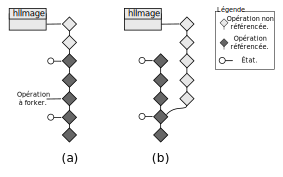
\includegraphics[width=\textwidth]{images/forking} 
			\label{fig:forking}
			\caption{Le forking d'une opération}
		\end{figure}

			Le résultat du forking est illustré à la figure~\ref{fig:forking}, page~\pageref{fig:forking}. Le schéma (a) montre la pile et l'opération
			que l'on désire forker. Le schéma (b) montre la nouvelle pile. 
			
			On constate donc que la pile n'a été dupliquée que depuis le sommet en cours, jusqu'à l'opération à forker, le reste de la pile 
			étant gardé commun, ceci permettant entre autre de réutiliser les caches des opérations communes. 

			En fait de pile, les opérations ressemblent désormais à une forèt. Mais il est impossible pour l'utilisateur du framework de s'en
			rendre compte. N'est visible depuis l'API publique qu'une simple pile et des états.

			L'intérèt de pouvoir référencer les opérations par uid apparait maintenant clair: Cela permet de référencer en tant que même 
			opération toutes les instances de celle-ci dans les différents états.  

			Le forking permet donc de concilier état et modifications pour une complexité temporelle et spatiale de $O(n)$ ou $n$ est le nombre
			d'opérations sauvegardées qui suivent l'opération à modifier.

			
		
	\section{Gestion de la cache}
		La gestion de la cache peut se résmuer en deux questions :
		\subsection{Quand et où mettre un tile dans la cache}
			Plus un tile est caché proche du sommet de la pile, plus il est efficace. Le sommet de la pile semble donc
			être un endroit de choix pour cacher les opérations. 

			Il est également utile de cacher les tiles sur les opérations référencées directement par un état, puisque
			celles-ci se retrouveront au sommet de la pile dès que l'état correspondant sera chargé. 

			Si l'on sait qu'une opération sera l'objet de modifications, il peut être intéressant de cacher à l'opération
			antérieure, afin d'accélérer la rasterisation après un fork. Pour savoir quelles opérations sont fréquemment
			modifiées, on s'en remet à l'utilisateur, qui peut marquer les opérations qu'il prévoit de modifier. 

			La consommation de mémoire est donc de l'ordre du nombre d'états et d'opérations modifiables se trouvant dans la pile.
		\subsection{Quand et quel tile enlever de la cache}
			\subsubsection{Tiles invalides}
			Il y a certains tiles que l'on \emph{doit} enlever de la cache; ceux qui ne sont plus valides. Il n'existe qu'une 
			seule façon d'invalider la cache d'une opération : modifier une opération antérieure. Ces tiles sont en fait
			automatiquement supprimés par les fonctions de modification de la pile.
			
			\subsubsection{Suppression d'états}
		\begin{figure}[ht]
			\centering
			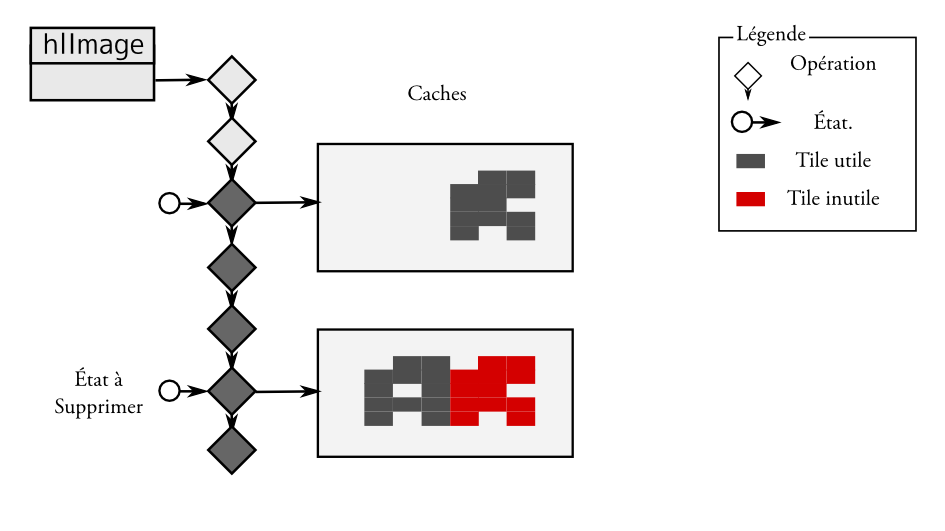
\includegraphics[width=\textwidth]{images/state-destruct} 
			\label{fig:destruct}
			\caption{Tiles inutiles après la suppression d'un état}
		\end{figure}
			Lorsqu'un état est supprimé, l'opération correspondante ne se trouvera plus jamais au dessus de la pile. On peut alors se
			demander s'il est intéressant de garder la cache de cette opération. Si l'opération ($A$) n'a pas été supprimée par la suppression
			de l'état, c'est qu'elle est référencée par un ou plusieurs autres états correspondant à des opérations ($C_i$), toutes postérieures à
			$A$. 

			A chaque tile caché de toute opération $B$, se trouvant entre $A$ et toutes les opérations $C_i$, correspond un tile caché dans $A$,
			qui est totalement inutile. En effet, tout rendu depuis les opérations $C_i$ atteindront les tiles des opérations $B$ avant d'atteindre
			les tiles de $A$. Ces tiles inutiles gaspillent de la mémoire et gagneraient à être supprimés.

			Il existe également des tiles de $A$ qui sont accessibles à partir d'une opération $C$, ceux-ci sont utiles, et gagneraient à être
			gardés. 

			Ceci est résumé par le schéma~\ref{fig:destruct}, page~\pageref{fig:destruct} qui représente en gris les tiles utiles et
			en rouge les tiles inutiles après la suppression d'un état.

			Il y a trois manières de gérer ce problème:
			\paragraph{a. Garder la cache}
				Dans ce cas, on consomme de la mémoire inutilement mais on évite de supprimer des tiles qui seront utiles par après.
				Les tiles se verront supprimés de la cache par un mécanisme global de suppression de tiles lorsque le framework manque
				de mémoire.

			\paragraph{b. Supprimer totalement la cache}
				Dans ce cas on libère toute la mémoire, mais on pourrait devoir recalculer certains tiles qui se trouvaient en cache.
				La complexité temporelle du rasterising revient donc à $O(n)$ ou $n$ est le nombre d'opération dans la pile. Heureusement,
				on atteint rarement ce cas en pratique. 

			\paragraph{c. Supprimer uniquement les tiles inutiles}
				Pour cela il faut tout d'abord trouver l'ensemble d'opération accessible depuis tous les $C_i$, ce qui n'est pas une chose 
				évidente puisque les références entre opérations vont dans l'autre sens. Dans le pire des cas la complexité spatiale
				et temporelle est de $O(n)$ ou $n$ est le nombre total d'opérations de toutes les piles correspondantes à cette image.
				La taille de l'ensemble d'opérations accessibles étant également en $O(n)$
				
				Enfin, pour chaque tile caché dans chacune de ces opérations, il faut supprimer les tiles des opérations correspondantes.
				Cette tâche se fait en $O(n*m)$ ou $n$ est la taille de l'ensemble d'opérations accessibles, et $m$ le nombre maximal de
				tile caché dans une opération. 

				Cette complexité semble prohibitive, mais il y a des cas particuliers qui se rencontrent souvent en pratique qui limitent
				fortement cette complexité. Il reste donc à savoir si les tiles utiles qui sont sauvegardés permettront 
				d'économiser plus de temps de calcul que celui qui est nécessaire pour réaliser cette opération. 

			Seules les solutions \emph{a} et \emph{b} ont été testées et implémentée. En raison de l'absence d'un dispositif global de suppression
			des tiles, c'est la solution \emph{b} qui a été retenue. 

			\subsubsection{Manque de mémoire}
			Enfin, il y a des moments ou l'on doit retirer des tiles de la cache car nous ne disposons plus de mémoire suffisante
			pour en stocker un nouveau. Aucun tile caché n'étant indispenable à la rasterisation du dessin, on peut supprimer ceux que l'on désire.
			
			Il faut donc trouver le tile le moins utile. il s'agit là d'un sujet vaste qui n'a pas encore été exploré
			ni implémenté. 
			
			Pour l'instant les tiles ne sont jamais retirés de la cache par manque de mémoire. Cela n'a pas posé de problèmes lors
			des tests utilisateurs, mais ceux-ci ne sont pas représentatifs d'une utilisation prolongée du framework. 

		\subsection{Migration de la cache}
			Il est également possible de migrer les tiles moins intéressant sur le disque dur, ou sur un espace réseau.
			Cette possibilité n'a pour l'instant pas été explorée ni implémentée.

	\section{Utilisation}
		Nous allons montrer dans cette section quelques examples qui illustrent l'utilisation de la structure et des algorithmes présentés
		dans ce chapitre afin de réaliser des fonctionalité utiles, ou d'émuler le fonctionnement d'autres frameworks. 
		\subsection{Undo / Redo}
			Pour implémenter l'undo redo, on va utiliser le système d'état. Après chaque modification de l'image correspondant à une action,
			on sauvegarde un nouvel état. On va ensuite placer cet état dans la "pile undo". 
			Lorsque la taille de cette "pile undo" dépasse le nombre maximal d'undo possible, on enlève le premier élément de celle-ci 
			et on détruit l'état correspondant. 

			Pour annuler une action, on charge l'état correspondant à une action antérieure. Pour refaire une action,
			on charge l'état correspondant à celle-ci. Lorsque l'on désire ajouter une action alors que l'on se trouve au milieu de la "pile undo",
			il faut supprimer tous les états se trouvant au dessus dans la pile. 

			Un tel système est efficace; les opérations de manipulations d'état sont suffisemment rapides pour que leur temps d'exécution
			soit imperceptible.
			
			La rasterisation après l'annulation ou le rétablissement d'une action est normalement en $O(1)$, grâce aux caches, 
			cependant, telle qu'implémentée, la gestion de la cache supprime des tiles utiles à la suppression d'états, ce qui peut occasionner
			quelques ralentissements. 
		\subsection{Modèle par calques}
		\begin{figure}[ht]
			\centering
			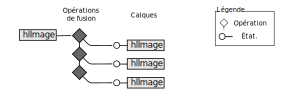
\includegraphics[width=\textwidth]{images/hl-calques} 
			\label{fig:hl-calques}
			\caption{Modèle par calques à partir d'hlImages.}
		\end{figure}
			Il est possible de construire un modèle par calque semblable à ceux utilisés par les frameworks bitmaps. A chaque calque correspond
			une hlImage. Une hlImage, regroupe ensuite les calques en utilisant des opérations de fusion. Ceci est représenté 
			sur le schéma~\ref{fig:hl-calques}, page~\pageref{fig:hl-calques}

		\subsection{Composition non linéaire}
		\begin{figure}[ht]
			\centering
			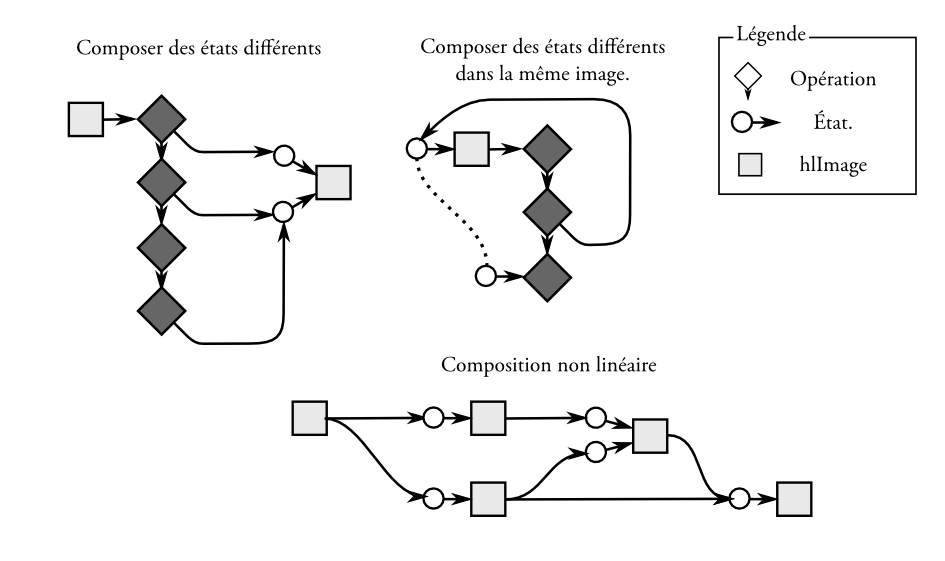
\includegraphics[width=\textwidth]{images/compnonlin} 
			\label{fig:compnonlin}
			\caption{Possibilités de composition non linéaire}
		\end{figure}
			Il existe deux façons de réaliser de la composition non linéaire: premièrement, plusieurs opérations de fusion peuvent référencer 
			la même image. Ensuite, les opérations de fusions référencent l'image à un état particulier, une opération de fusion n'ayant pas
			besoin de charger un état dans une image pour la rasteriser. Il est ainsi possible de référencer la même image à des états différents.

			Il est également possible pour une image de se référencer elle même à différents états, tant que cela ne crée pas de boucle. 

			En utilisant les opérations de fusion et les états, le framework Himalaya offre des possibilités de composition non linéaire très
			proches de ce qu'offre un framework nodal. 

			Ces possibilités sont résumées au schéma~\ref{fig:compnonlin}, page~\pageref{fig:compnonlin}.

\chapter{Localité des operations (20 pages)}
	\section{Opérations vectorisées}
		\subsection{Impact sur l'API}
		\subsection{Évaluation des performances}
	\section{Bounding Boxes}
		\subsection{Algorithme Inline}
		\subsection{Algorithme Off-line}
		\subsection{Multi-Niveaux}
		\subsection{Impact sur l'API}
		\subsection{Évaluation des performances}

\chapter{Anti-aliasing (15 pages) }
	\section{Primitive de dessin}
	\section{Problèmes d'échelle}
		\subsection{Oversampling}
	\section{Problèmes de superposition}
	\section{Problèmes de bandes}
	\section{Problème de blending à faible opacité}
	\section{Problème de précision de positionement}
\chapter{Test utilisateurs (10 pages) }
	\section{Procédure}
	\section{Résultats}
	\section{Analyse}
\chapter{Comparaison d'Himalaya aux autres frameworks}
\chapter{Conclusion}

	\chapter{Localité des opérations}
	Ce chapitre traite de la gestion de la localité des opérations. Une
	opération est dite locale si elle n'affecte qu'une sous-région de l'image.

	Il est rapidement apparu que la gestion de ces opérations par l'algorithme
	de rasterisation présenté à la section précédente était loin d'être optimale,
	et ne permettait pas d'atteindre les objectifs d'interactivité du logiciel.

	Pour comprendre le problème, il faut d'abord comprendre comment fonctionne le
	logiciel de peinture. 
	\section{Le logiciel de peinture}
		Le logiciel de peinture possède trois outils principaux : La peinture,
		l'undo/redo, et une fenêtre de visualisation.
		\subsection{Background}
			Le logiciel présente à l'utilisateur une zone de dessin constituée d'un
			rectangle blanc qui représente la feuille sur laquelle dessiner. 
			Pour ce faire, nous utilisons une Frame unie et transparente comme source
			de l'hlImage, à laquelle nous ajoutons une opération de dessin d'un
			rectangle blanc. 
		\subsection{Peinture}
			La peinture se fait par la superposition de primitives appelées \emph{brushes}
			positionnées
			à intervalles réguliers sur le chemin tracé par l'utilisateur via la
			souris ou la tablette graphique. Les opérations de dessin de primitives 
			sont regroupées en traits, qui correspondent à une pression 
			continue sur le dessin. 

			La primitive utilisée pour la peinture est le cercle avec dégradé. Celui-ci
			est défini par deux rayons: Le rayon interne dans lequel le cercle est opaque,
			et le rayon externe, auquel se termine le cercle. Entre les deux un dégradé
			transparent. L'utilisateur peut aussi régler 
			l'opacité et la couleur de la primitive.

			Toutes les opérations sont ajoutées dans une seule hlImage, dont l'état
			est sauvegardé à chaque fin de trait.
		\begin{figure}[ht]
			\centering
			\includegraphics[width=\textwidth]{images/draw} 
			\caption{Fonctionnement de la peinture}
			\label{fig:draw}
		\end{figure}

			Ce mécanisme est résumé au schéma~\ref{fig:draw}, page~\pageref{fig:draw}.
			
		\subsection{Undo/Redo}
			L'undo redo fonctionne de la manière décrite au chapitre précédent.
			Une pile maintient une liste des états de chaque traits, permettant de défaire
			et refaire les opérations. 

			Comme indiqué au chapitre précédent, la consommation de mémoire est de
			l'ordre du nombre d'états. Comme il n'y a pas de mécanisme permettant de
			réguler les caches de manière globale, nous limitons le nombre d'états --- et donc d'undos --- disponibles
			à 16.
		\subsection{Visualisation}
			L'utilisateur visualise son dessin en temps réel via une fenêtre de visualisation.
			Celle-ci est décrite par sa taille en pixels, sa position sur le dessin, ainsi
			que son niveau d'échelle. 
			
			À chaque rafraîchissement (entre 30 et 60 fois par secondes), les tiles correspondant
			à la région sont identifiés, rasterisés, et copiés dans le buffer correspondant à la région
			afin d'être visualisés. 

			Les rafraîchissement se font indépendemment de l'ajout d'opérations. Un nombre quelconque
			d'opération peut donc avoir été ajouté entre deux rasterisations de l'image.

			L'utilisateur peut modifier la région de visualisation de trois manières différentes :

			\begin{itemize}
				\item Déplacer la région.
				\item Redimensionner la région.
				\item Changer l'échelle de visualisation.
			\end{itemize}

			Alors que déplacer et redimensionner la région ne demande que de recalculer les quelques tiles de la nouvelle
			bordure, changer l'échelle demande de recalculer l'entièreté de la région de visualisation. On peut
			donc s'attendre à ce que le déplacement et le redimensionnement de la région de visualisation soient 
			beaucoup plus rapides que le changement d'échelle.

	\section{Problématique}
		L'algorithme de rasterisation présenté jusqu'ici n'a aucune notion de localité d'opérations. Quelque soit le tile
		que nous voulons rasteriser, l'algorithme va appeler chacune des opérations. Si ces opérations ne s'appliquent pas
		au tile, celles-ci ne vont pas le modifier et vont donc s'exécuter très rapidement. Cependant, dans le cas de la 
		peinture, chaque tile n'est en réalité affecté que par un très petit pourcentage des opérations, et le nombre
		d'appel à ces opérations inutiles va en pratique ralentir de manière substantielle la rasterisation.

		Ce cas est particulièrement problématique lors du déplacement de la région de visualisation. Après avoir fait
		un large nombre de traits de peinture dans la région courante, l'utilisateur décide de déplacer la région de
		visualisation. De nouveaux tiles doivent donc être affichés. Pour ce faire l'algorithme de rasterisation va 
		examiner toutes les opérations des traits que l'utilisateur vient de dessiner, alors qu'aucun de ces traits n'affectent
		ces nouveaux tiles. 

		Il faut donc permettre à l'algorithme de rasterisation de pouvoir éviter d'examiner toute opération qui n'affecte
		pas les tiles. Au lieu d'avoir un algorithme de rasterisation en $O(n)$ ou $n$ est le nombre d'opérations
		ajoutées depuis le dernier rendu, nous aimerions avoir pour $n$ le nombre d'opérations ajoutées depuis le dernier
		rendu \emph{qui affectent le tile}.

		Il n'a pas été possible durant ce mémoire de trouver une réponse définitive à ce problème. Nous allons donc 
		passer en revue les différentes options qui ont été considérées, ainsi que leur efficacité. L'analyse de leur
		efficacité nous permet d'avoir une bonne idée de la direction à prendre pour la poursuite des recherches d'une
		solution à ce problème.

		Deux approches ont été testées: Les opérations vectorisées et les bounding operations. 	


	\section{Bounding Boxes}
\newcommand{\BB}{\emph{BB}~}
		Une première étape est d'ajouter à toutes les opérations de dessin une \emph{Bounding Box} --- \BB en abrégé.
		Celle-ci représente
		Une région rectangulaire, alignée aux axes de l'image, comprenant les tiles affectés par l'opération. Avant de rasteriser une opération 
		sur un tile, la \BB est examinée pour voir si le tile est affecté. s'il ne l'est pas, on peut éviter 
		de faire appel à la fonction de l'opération qui aurait de toute manière implémenté un tel mécanisme 
		de manière interne.

		Un autre intérêt d'un tel système est que la \BB est générée à la création de l'opération, et non à
		chaque appel de l'opération, ce qui améliore encore les performances.
		
		Pour réaliser cela, chaque classe d'opération doit donc être capable de générer de telles \BB.

		Si les \BB améliorent nettement les performances, elles n'améliorent pas la complexité
		temporelle de la rasterisation. Elles constituent cependant une base solide pour les deux solutions suivantes. 

	\section{Opérations vectorisées}
		\begin{figure}[ht]
			\centering
			\includegraphics[width=\textwidth]{images/vector} 
			\caption{(a) Opérations normales, (b) Opérations vectorisées}
			\label{fig:vector}
		\end{figure}
		Vectoriser les opérations consiste à regrouper des opérations du même type en une seule opération qui contient
		un vecteur de paramètres représentant l'ensemble des paramètres. La \BB de l'opération
		vectorisée englobant les \BB des opérations qui la composent. Ceci est représenté au 
		schéma~\ref{fig:vector}, page~\pageref{fig:vector}
		Les opérations vectorielles ont plusieurs intérêts:
		\begin{itemize}
			\item La structure hlOperation est mise en commun, permettant d'économiser la mémoire.
			\item Si un paramètre des opérations est constant dans le vecteur, celui-ci peut être mis en commun,
			ce qui économise de la mémoire. Ce cas de figure se présente régulièrement en peinture; les traits étant principalement
			composés de \emph{brushes} de même couleur et de même diamètre.
			\item Un test sur la Bounding box de l'opération vectorielle permet d'éviter le test de l'intégralité
			des opérations internes.
		\end{itemize}
		Mais ne sont pas sans limites:
		\begin{itemize}
			\item Il n'est pas possible de vectoriser des opérations de type différent. Ce système ne fonctionnerait
			donc pas pour un pinceau qui peindrait une alternance de cercles et de carrés.
			\item Il n'est pas possible de placer un état au milieu d'opérations vectorisées.
			\item L'algorithme de rasterisation doit être lourdement modifié pour pouvoir supporter ce type d'opérations.
			\item Les opérations vectorisées ne peuvent être modifiées avec l'API classique.
		\end{itemize}
				\begin{table*}
					\centering
					\begin{tabular*}{0.7\textwidth}{@{\extracolsep{\fill}} | c | c |}
					\hline
					Dessin & Nombre moyen d'opérations par trait \\
					\hline
					A	& 105.4 \\
					B	& 199.8 \\
					C	& 117.8 \\
					D	& 149.1 \\
					E	& 117.2 \\
					\hline
					\end{tabular*}
					\caption{Nombre moyen d'opérations par trait sur les dessins de tests (voir figure~\ref{fig:testdrawings}, 
					page~\pageref{fig:testdrawings}) }
					\label{strokelength}
				\end{table*}
		Les performances des opérations vectorisées seront donc contraintes par le nombre d'opérations du même type que
		l'on trouve entre chaque état. Pour l'application de peinture développée, les opérations sont toujours du même
		type, et un trait faisant en moyenne une centaine d'opérations (voir tableau~\ref{strokelength}, page~\pageref{strokelength}), 
		le nombre de tests de bounding box à réaliser en 
		dehors des traits est divisé par 100. Le nombre de tests à réaliser sur les traits, augmente en contrepartie d'un
		pourcent à cause de la \BB supplémentaire.

		Nous n'atteignons donc pas notre objectif de réduction de complexité, mais les opérations vectorisées permettent
		de réduire de deux ordres de grandeur le coût de la localité des opérations.

		\subsection{Impact sur l'API}
		Étant donné les limitations des opérations vectorisées, nous sommes obligés de donner à l'utilisateur un
		certain contrôle sur celles-ci. Nous proposons donc une fonction supplémentaire :
			\paragraph{\lstinline$void hlOpVectorise(hlOperation *op)$}
			\begin{description}
				\item[pre]: op est une opération qui n'est pas encore insérée dans la pile.
				\item[post]: op est une opération vectorisée. Toute opération non vectorisée du même
				type qu'op insérée sur la pile au dessus de op sera vectorisée dans op, jusqu'à ce
				que op soit sauvegardée dans un état.
			\end{description}
		Ainsi, l'utilisateur n'a qu'à utiliser cette fonction sur la première opération de chaque trait pour pouvoir
		vectoriser les traits. 
		\subsection{Évaluation des performances}
		À part un gain de mémoire au niveau de la description du document, qui reste négligeable par rapport au poids pris
		par les caches, les performances démontrées par les opérations vectorisés sont quasiment identiques à un cas particulier
		des Bounding Opérations, solution plus prometteuse présentée à la section suivante.

		Nous nous référerons donc à la section \emph{Évaluation des performances / Tailles des \emph{BO}} 
		pour un aperçu des performances des opérations vectorisées.  

	\section{Bounding Opérations}
\newcommand{\BO}{\emph{BO}~}
		\begin{figure}[ht]
			\centering
			\includegraphics[width=\textwidth]{images/bo} 
			\caption{Une Bounding Opération}
			\label{fig:bo}
		\end{figure}
		Les \emph{Bounding Opérations} -- \BO en abrégé --- ne sont pas des opérations au sens original du terme puisque si utilisées
		correctement, elles n'effectuent aucune modification de l'image. Cependant elles s'utilisent et s'insèrent
		dans la pile comme des opérations classiques  appartenant à une nouvelle catégorie.  Leur but est d'offrir une \BB englobant
		plusieurs opérations, de la même manière que les opérations vectorisées, mais de manière plus flexible et facile à implémenter:

		\subsection{Principes d'une \BO}
		
		Les \BO contiennent une \BB et une référence vers une opération antérieure.
		La rasterisation des \emph{Bounding Opérations} fonctionne de la manière suivante:
		\begin{itemize}
			\item Rasteriser un tile à l'intérieur de la \BB consiste à rasteriser l'opération précédente.
			\item Rasteriser un tile à l'extérieur de la \BB consiste à rasteriser l'opération antérieure référencée.
		\end{itemize}

		En créant une \BO dont la \BB englobe les \BB d'une suite
		d'opérations qui la précèdent, et en faisant pointer la \BO sur une opération précédant 
		cette suite, on permet à l'algorithme de rasterisation de contourner la suite d'opérations.
		
		Ce principe est représenté au schéma~\ref{fig:bo}, page~\pageref{fig:bo}

		Les \BO ne modifiant pas l'apparence de l'image, on peut les placer où l'on veut dans la pile. Ces 
		opérations peuvent donc "enjamber" des états, permettant des groupements qui ne sont pas possibles avec les opérations
		vectorisées.

		\begin{figure}[ht]
			\centering
			\includegraphics[width=\textwidth]{images/bo2} 
			\caption{Une Bounding Opération Hierarchy}
			\label{fig:bo2}
		\end{figure}

		Là où les \BO deviennent très intéressantes c'est qu'on peut les emboîter les unes dans les
		autres de manière récursive, et ainsi offrir une structure semblable à une \emph{Bounding Volume Hierarchy}\cite{shirley} 
		--- \emph{BVH} en abrégé --- ou à des \emph{KD-Trees}\cite{shirley}. On appelle \emph{Bounding Opération Hierarchy} --- \emph{BOH}
		en abrégé --- L'implémentation par des \BO de ce type de structures. Lorsque les \BO ne s'imbriquent pas, on parle alors de \emph{Bounding Object Sequence},
		--- \emph{BOS} en abrégé. Un exemple de \emph{BOH} est représenté au schéma~\ref{fig:bo2}, page~\pageref{fig:bo2} 

		\begin{figure}[ht]
			\centering
			\includegraphics[width=\textwidth]{images/bo3} 
			\caption{Cas critique pour les \emph{BOH}}
			\label{fig:bo3}
		\end{figure}
		Il y a cependant une grande différence entre les \emph{BVH}, et les \emph{BOH}; là où un \emph{Bounding Volume}
		peut contenir n'importe quel ensemble
		d'objets dans la scène, une \BO ne peut contenir que des opérations qui sont adjacentes dans la pile. Il
		est très simple de construire un exemple ou les \emph{BVH} excellent et les \emph{BOH} ne font qu'empirer
		les choses, comme sur le schéma~\ref{fig:bo3}, page~\pageref{fig:bo3}. Heureusement de tels cas arrivent peu 
		en pratique, puisque les outils de peinture tendent à grouper les opérations de manière adéquate.

		Il serait cependant possible d'approcher l'efficacité d'un \emph{BVH} en procédant à un réordonancement intelligent
		des opérations. 
		
		Une autre différence de taille est que les \emph{BVH} sont conçus pour organiser des scènes statiques,
		et non pour des scènes pouvant changer selon les états. Ces différences nous empêchent de reprendre 
		les algorithmes développés pour les \emph{BVH} et les \emph{KD-Trees}, 
		même si nous pouvons en reprendre les idées et les principes. 

		Une première tâche intéressante consiste à construire la \emph{BOH}. La littérature\cite{havran} sur les \emph{BVH}
		décrit deux types d'algorithmes:
		\begin{description}
			\item[Algorithmes Inline] Ces algorithmes construisent la \emph{BVH} au fur et à mesure
			que l'on ajoute des objets dans la scène --- des opérations dans l'image. Ces algorithmes 
			semblent donc particulièrement adaptés à la peinture puisqu'ils fonctionneront au fur et à mesure que l'utilisateur
			peint. Ces algorithmes 
			\item[Algorithmes Offline] Ces algorithmes construisent la \emph{BVH} à partir d'une 
			scène déjà construite --- d'un pile d'opération existante. Ces algorithmes ont l'avantage de pouvoir
			créer des hiérarchies optimales (selon différents critères). Le problème est qu'ils prennent un certain temps 
			à s'exécuter, ce qui n'est pas idéal pour un framework dédié à l'édition interactive. 
		\end{description}
		Seul des algorithmes inline ont pour l'instant été explorés et implémentés. Un algorithme crée des \emph{BOS} ,
		et l'autre des \emph{BOH}. 
		
		\subsection{Bounding Opération Sequence}
			Le premier algorithme testé et implémenté est un algorithme créant un \emph{BOS}
			
			\subsubsection{Placement des \BO dans la pile}
			Le placement des \BO dans la pile fonctionne de la manière suivante: Initialement, la \BO possède une \BB
			de taille nulle, et est dans l'état dit \emph{ouvert} Lorsque l'on insère cette \BO au dessus de la pile, 
			celle-ci prend pour comme opération de référence l'opération précédente. 

			Lorsque l'on insère une opération sur la pile, au dessus d'une \BO ouverte, la \BB de la \BO est étendue
			pour englober la \BB de la nouvelle opération. La \BB est ensuite repositionnée au dessus de la pile. 

			L'on peut continuer à insérer des opérations de cette manière jusqu'à ce que la \BO soit \emph{fermée},
			auquel cas elle se comporte comme une opération normale. 

			\subsubsection{Fermer les \emph{Bounding Opérations}}
			Ce premier algorithme va donc ajouter des \BO ouvertes, les fermer au moment opportun et puis directement 
			en rajouter une nouvelle ouverte. Il s'agit donc de savoir quand fermer les \BO.

			L'impact des performances des \BO peut se répartir en deux cas\footnote{cette discussion est équivalente à celles motivant les \emph{Bounding Area Heuristics} utilisées pour la construction de \emph{KD-Trees} ou \emph{BVH}\cite{havran}} :
			\begin{description}
				\item[Rendu d'un tile à l'extérieur de la \BO]: Dans ce cas, on doit effectuer un test de \BB de la \BO
				uniquement. Comme on aimerait diminuer le nombre de tests de \BB, on aimerait donc avoir un nombre minimal
				de \BO.
				\item[Rendu d'un tile à l'intérieur de la \BB]: Dans ce cas, on doit tester les \BB de toutes les 
				opérations à l'intérieur de la \BO, que celles ci influence le tile ou pas. On aimerait donc avoir le moins
				de Rendus à l'intérieur de \BO. Statistiquement, plus la surface de la \BB d'une \BO est petite, moins de
				tiles seront rendus à l'intérieur. On aimerait donc avec des \BO avec les \BB les plus petites possibles.
			\end{description}
			
			La fermeture des \BO doit donc satisfaire deux critères: avoir le moins de \BO, et avoir les \BO les plus petites. 
			Ces deux critères étant opposés, nous allons examiner leur importance en examinant différents schémas de fermeture
			dans la section \emph{analyse de performances}
			

		\subsection{Bounding Opération Hierarchy}
			Cet algorithme permet de créer une hiérarchie de \BO d'une profondeur fixe. Dans cet algorithme chaque niveau
			fonctionne exactement comme l'algorithme précédent en considérant les \BO des opérations d'en dessous comme
			des opérations classiques. Une première analyse d'efficacité se trouve à la section \emph{Analyse des performances}


		\subsection{Impact sur l'API}
			Les \BO ont un impact minimal sur l'API. Il suffit d'ajouter une opération de type \BO avec les paramètres
			appropriés pour que les mécanismes se mettent en place. Une fois en place les \BO n'influent quasiment pas
			sur les actions que l'on peut réaliser sur une hlImage. 

			Par contre, le fait que les \BO puissent être déplacées automatiquement par d'autres opérations perturbe
			l'accès aux opérations par indice. Pour résoudre ce problème, les \BO sont ignorées lors des accès par
			indice. 

			Si l'algorithme de rasterisation ne doit pas être grandement modifié, les algorithmes de modification
			de la pile doivent être revus pour préserver la cohérence des \emph{BOH}.

			\subsubsection{Forking}
			\begin{figure}[ht]
				\centering
				\includegraphics[width=\textwidth]{images/bo-forking} 
				\caption{Forker des \BO}
				\label{fig:bo-forking}
			\end{figure}
			L'opération de forking doit duplique également les \BO. Le schéma~\ref{fig:bo-forking}, page~\pageref{fig:bo-forking} montre une pile
			contenant des \BO avant et après forking. 

			La difficulté réside donc à réassocier les références correctement. 
			Ceci se fait en reprenant l'algorithme de forking en appliquant les modifications suivantes:
			\begin{itemize}
				\item Lorsque l'on duplique une \BO, son duplicata continue à pointer vers l'opération originale.
				On associe ensuite dans une Hashtable l'uid de l'opération pointée
				par la \BO à cette \BO. 
				\item Lorsque l'on duplique une opération (\BO comprises), on regarde si son uid est présente dans
				la Hashtable. Dans l'affirmative, la \BO correspondante pointe désormais sur cette opération, et
				l'uid est retiré de la Hashtable.
			\end{itemize}
			L'opération de forking garde donc toujours la même complexité temporelle, mais gagne une complexité spatiale
			de $O(n)$ où $n$ est la profondeur maximale de la \emph{BOH}, la profondeur des \emph{BOH} étant en $O(log(n))$, où $n$
			est le nombre total d'opérations dans la pile. 
			
			\subsubsection{Retrait d'opérations}
			\begin{figure}[ht]
				\centering
				\includegraphics[width=\textwidth]{images/bo-supress} 
				\caption{Retirer une opération pointée par une \BO}
				\label{fig:bo-supress}
			\end{figure}
			Le retrait d'une opération dans la pile peut être problématique si un \BO pointe sur cette opération. Dans de
			tel cas, il faut détecter les \BO qui pointent et les faire pointer vers l'opération précédente à celle
			que l'on veut retirer. Si il n'y a pas de telle opération précédente, on met la référence à \emph{NULL} pour indiquer qu'il faut accéder directement à la source de l'image.
			Il faut également supprimer les \BO qui ne contiennent d'opération autre
			que des \BO.  Un exemple de retrait d'opération dans une pile contenant des \BO est représenté au 
			schéma~\ref{fig:bo-supress}, page~\pageref{fig:bo-supress}
			
			Ceci ne modifie pas la complexité temporelle, mais ajoute une complexité spatiale
			de $O(n)$ ou $n$ est le nombre de \BO pointant l'opération à retirer. Ce nombre est également borné par
			la profondeur de la \emph{BOH}, ce qui ramène cette complexité à $O(log(n))$ ou $n$ est le nombre d'opérations dans
			la pile jusqu'à l'opération à retirer. 

			\subsubsection{Insertion et Modification d'opérations}
			\begin{figure}[ht]
				\centering
				\includegraphics[width=\textwidth]{images/bo-modify} 
				\caption{Modifier une opération dans une pile contenant des \BO}
				\label{fig:bo-modify}
			\end{figure}
			Insérer ou modifier des opérations peut invalider les \BB des \BO qui englobent ces opérations. Il faut
			donc détecter ces \BO, et modifier leur \BB afin qu'elles contiennent la \BB de l'opération à insérer, ou la
			nouvelle \BB de l'opération modifiée, ce qui se fait en parcourant la pile jusqu'à l'emplacement d'insertion,
			ou jusqu'à l'opération à modifier de la manière suivante
			\begin{itemize}
				\item Lorsque l'on rencontre une \BO, on l'associe dans une Hashtable à l'opération pointée.
				\item Lorsque l'on rencontre une opération, on retire la \BO associée dans la Hashtable.
				\item Lorsque l'on arrive à l'emplacement voulu, ou à l'opération à modifier, la Hashtable
				contient la liste des \BO à modifier.
			\end{itemize}
			Cela ne modifie donc pas la complexité temporelle, mais ajoute une complexité spatiale, en $O(log(n))$ où $n$
			est le nombre d'opérations dans la pile.

		\subsection{Évaluation des performances}
			Pour évaluer les performances, nous avons enregistré les étapes de création de plusieurs dessins, chacun d'entre eux représentant
			un cas d'utilisation différent. Ces dessins de taille variable ont été réalisés sur une feuille de $4.8*10^{17}$ pixels. Nous avons 
			ensuite rejoué ces étapes (ajout d'opérations, rasterisation, zoom, dézoom, undo, redo,
			déplacement du viewport) en omettant les pauses afin de mesurer le temps total pris par le framework pour dessiner le dessin.
			
			Toutes les expériences ont été réalisées sur une machine disposant d'un processeur \emph{Intel Core Duo 2400} à deux cores cadencés
			à 1.66GHz, et disposant de 2Go de mémoire vive. 

			\begin{figure}[h]
				\centering
				\captionsetup[subfigure]{labelformat=empty}
				\subfloat[$(a)$~Dessin technique, 25Mpixels]{ \includegraphics[width=0.5\textwidth]{images/tests/test_a} }
				\subfloat[$(b)$~Hachures, $0.5$Gpixels]{ \label{fig:testb} \includegraphics[width=0.5\textwidth]{images/tests/test_b} }
				\\
				\subfloat[$(c)$~Portrait, $25$Mpixels]{ \label{fig:testc} \includegraphics[width=0.5\textwidth]{images/tests/test_c} }
				\subfloat[$(e)$~Test divers, $0.5$Gpixels]{ \label{fig:teste} \includegraphics[width=0.5\textwidth]{images/tests/test_e} }
				\\
				\subfloat[$(d)$~Paysage avec petits détails, $2$Gpixels]{ \label{fig:testd} \includegraphics[width=\textwidth]{images/tests/test_d} }
				\caption{Dessins utilisés pour les tests de performances}
				\label{fig:testdrawings}
			\end{figure}

			Les cinq dessins sont présentés à la figure~\ref{fig:testdrawings}, page~\pageref{fig:testdrawings}. Chacun d'entre eux a été
			réalisé pour simuler un cas d'utilisation différent:
			\begin{description}
				\item[A] Ce dessin représente un dessin technique, composé essentiellement de lignes droites d'orientation similaires, ainsi
				que d'arcs de cercles. 
				\item[B] Ce dessin représente des hachures, qui peuvent constituer l'essentiel d'un dessin au trait.
				\item[C] Ce portrait est destiné à représenter un dessin complet qui comprend une variété de technique différentes : traits de contour,
				remplissages, hachures, ...
				\item[D] Ce paysage de grande taille contenant de très petits éléments simule l'utilisation du framework pour l'édition d'images
				gigapixel à des échelles fort différentes.
				\item[E] Ce dessin est constitué de différents éléments ayant posé problèmes lors des tests de performances, comme par exemple 
				des brushes et des traits de taille très différentes. 
			\end{description}
			Ces dessins sont en noir et blanc pour limiter le nombre d'opération nécessaires à leur réalisation. En effet les dessins ont été faits 
			suffisamment petits pour limiter le temps de calcul lors de l'évaluation des performances. Ces dessins ne sont donc pas totalement
			représentatifs de ce qui se fait en conditions réelles, mais devraient être suffisamment proche pour nous permettre de savoir quelle
			solutions gagneraient à être explorées plus en détail sur des données en provenance de tests utilisateurs.

			\subsubsection{Taille des \BO}
				Le premier test utilise une heuristique qui ferme la boite quand celle-ci contient un certain nombre d'opérations, ou
				quand un nouvel état est enregistré. À noter que cette heuristique correspond exactement au système d'opération vectorisées,
				qui produit des temps de calculs quasiment identiques. 

				\begin{table*}
					\tiny
					\begin{tabular*}{\textwidth}{@{\extracolsep{\fill}} | c || c | c | c | c | c | c | c | c | c | c |}
						\hline
						& \multicolumn{10}{c|}{Nombre maximal d'opérations par \BO} \\
						\hline
								&8		&  16		&  32		&  64		&  128		&  256		&  512		&  1024		&  2048		&  4092		 \\
						\hline
						\hline
						Dessin & \multicolumn{10}{c|}{Temps de calcul (sec)} \\
						\hline
						 A		& 249.67	&  117.81	&  72.01	&  52.00	&  39.13	&  34.32	&  32.87	&  32.84	&  32.99	&  32.83	 \\
						 B 		& 847.67	&  312.65	&  113.12	&  70.14	&  52.35	&  40.44	&  39.45	&  41.32	&  42.51	&  42.78	 \\
						 C		& 1283.64	&  550.17	&  354.88	&  154.36	&  138.46	&  163.26	&  104.11	&  94.40	&  108.18	&  146.60	 \\
						 D		& 1181.11	&  466.45	&  278.11	&  144.25	&  170.93	&  132.44	&  91.03	&  89.84	&  88.35	&  140.39	 \\
						 E		& 61.32		&  38.71	&  18.21	&  12.93	&  11.81	&  11.19	&  11.01	&  11.08	&  10.72	&  11.15	 \\
						\hline
					\end{tabular*}
					\caption{\label{boxdepth} Performances de la première heuristique de fermeture des \BO}
				\end{table*}
				\begin{figure}[h]
					\centering
					\includegraphics[width=\textwidth]{images/depthgraph.eps} 
					\caption{\label{fig:depthgraph}Peformances de la première heuristique normalisées par leur meilleur temps}
				\end{figure}
				
				Le tableau~\ref{boxdepth}, page~\pageref{boxdepth}, reprend les résultats des expériences pour différentes tailles de boites.
				Le graphe~\ref{fig:depthgraph}, page~\pageref{fig:depthgraph} reprend ces données en normalisant les durées d'exécution de chaque
				test sur la durée la plus rapide. 

				On peut y voir que les performances augmentent avec la taille des \BO pour ne jamais redescendre. On en déduit donc que 
				la taille de la boite importe beaucoup moins que leur nombre. Si les performances ne diminuent pas plus au delà d'un
				certain nombre d'opérations par \BO, c'est parce qu'à partir d'un certain point, les \BO sont toutes fermées par 
				l'enregistrement d'un nouvel état. 

			\subsubsection{Aire accumulée}
				Cette heuristique basée sur l'aire accumulée essaie d'établir un compromis entre la taille des \BO et le nombre d'opérations
				contenues dans celles-ci:

				A chaque fois que l'on insère une opération dans une \BO, on évalue l'augmentation de la surface de la \BB de celle-ci. 
				On normalise ensuite cette augmentation de surface par la taille de la \BB de l'opération ajoutée. Cette augmentation
				de surface est accumulée dans un compteur dans la \BO. Lorsque celle-ci dépasse un seuil, la \BO est fermée. 

				Cette heuristique favorise donc des \BO plus denses, ce qui l'on espère, permettra d'avoir une meilleure répartition des
				\BO.

				\begin{table*}
					\tiny
					\begin{tabular*}{\textwidth}{@{\extracolsep{\fill}} | c || c | c | c | c | c | c | c | c |}
						\hline
						& \multicolumn{8}{c|}{Aire maximale accumulée par \BO} \\
						\hline
								& 2		& 4		& 8		&  16		&  32		&  64		&  128		&  512		\\
						\hline
						\hline
						Dessin & \multicolumn{8}{c|}{Temps de calcul (sec)} \\
						\hline
						A		& 70.85		&  51.89	&  41.54	&  37.51	&  35.72	&  34.89	&  36.23	&  54.46	\\
						B		& 225.32	&  139.10	&  100.74	&  83.29	&  45.69	&  42.70	&  41.45	&  43.58	\\
						C		& 585.40	&  321.23	&  141.87	&  163.36	&  156.43	&  145.06	&  143.24	&  141.66	\\
						D		& 656.04	&  358.37	&  158.52	&  153.24	&  159.39	&  149.18	&  148.01	&  98.38	\\
						E		& 16.21		&  12.59	&  11.73	&  12.30	&  11.44	&  10.62	&  11.13	&  10.66	\\
						\hline
					\end{tabular*}
					\caption{\label{boxratio} Performances de la seconde heuristique}
				\end{table*}
				\begin{figure}[h]
					\centering
					\includegraphics[width=\textwidth]{images/graph_ratio.eps} 
					\caption{\label{fig:ratiograph}Performances de la seconde heuristique normalisées par leur meilleur temps}
				\end{figure}
				Les résultats des expériences sont repris au tableau~\ref{boxratio}, page~\pageref{boxratio}. Celles-ci sont également
				reprises normalisées sur leur meilleur temps au graphe~\ref{fig:ratiograph}, page~\pageref{fig:ratiograph}.

				On constate tout d'abord que cette heuristique ne permet pas d'atteindre les temps atteints par la précédente. On constate
				ensuite que l'évolution des améliorations est moins régulière et reflète les différences de structure des différentes images. 
				Cette évolution irrégulière a pour conséquence qu'aucune valeur n'est optimale pour tous les tests, indiquant que la limite doit
				être modulée en fonction de l'utilisation du framework. 

				On constate également que cette heuristique fonctionne le moins bien pour les images \emph{A} et \emph{C}, qui contiennent
				beaucoup de diagonales.  Le problème de cette heuristique avec ces diagonales c'est que celles-ci sont particulièrement mal
				épousées par les \BB qui sont alignées aux axes. Dans ces cas l'aire est accumulée quadratiquement avec la longueur, et donc
				les boites sont clôturées trop tôt. Ceci génère un trop grand nombre de \BO, et comme le résultat de l'expérience précédente
				nous indique, les performances sont fortement affectées lorsque celles-ci sont trop nombreuses.

			\subsubsection{\emph{BOH}}
				Nous utilisons pour cette troisième heuristique une \emph{BOH} à deux niveaux. Les \BO du premier niveau se clôturent
				au delà d'un nombre fixe d'opérations, de la même manière que la première heuristique. Les \BO du second niveau ne sont
				quand à elles clôturées qu'à l'ajout d'un nouvel état. Cette heuristique permet donc d'évaluer les gains que l'on peut
				obtenir en rajoutant un second niveau. 
				\begin{table*}
					\tiny
					\begin{tabular*}{\textwidth}{@{\extracolsep{\fill}} | c || c | c | c | c | c | c | c | c | c | c |}
						\hline
						& \multicolumn{10}{c|}{Nombre maximal d'opérations par \BO} \\
						\hline
								&8		&  16		&  32		&  64		&  128		&  256		&  512		&  1024		&  2048		&  4092		 \\
						\hline
						\hline
						Dessin & \multicolumn{10}{c|}{Temps de calcul (sec)} \\
						\hline
						A		& 56.33		&  35.43	&  33.72	&  33.41	&  33.57	&  33.32	&  32.82	&  34.31	&  34.76	&  34.26	\\
						B		& 53.30		&  70.24	&  67.47	&  66.61	&  64.70	&  41.40	&  42.01	&  43.41	&  44.54	&  44.36	\\
						C 		& 107.27	&  144.32	&  141.42	&  94.17	&  91.31	&  123.96	&  142.79	&  141.63	&  142.71	&  148.53	\\
						D		& 144.20	&  88.20	&  86.48	&  115.26	&  140.11	&  147.81	&  141.73	&  101.48	&  88.51	&  108.78	\\
						E		& 17.88		&  17.06	&  16.89	&  16.67	&  16.32	&  16.59	&  16.51	&  16.59	&  16.88	&  16.28	\\
						\hline
					\end{tabular*}
					\caption{\label{boxdepth1}Performances de la troisième heuristique}
				\end{table*}
				\begin{figure}[h]
					\centering
					\includegraphics[width=\textwidth]{images/depthgraphd1.eps} 
					\caption{\label{fig:depthgraphd1}Performances de la troisième heuristique normalisées par leur meilleur temps}
				\end{figure}
				Les résultats sont résumés dans le tableau~\ref{boxdepth1}, page~\pageref{boxdepth1}, et repris sous forme normalisée par leur
				meilleur résultat au graphe~\ref{fig:depthgraphd1}, page~\pageref{fig:depthgraphd1}. 

				On constate que les différences de structure des dessins crée une grande variation dans les performances en fonction de
				la taille des \BO internes, ainsi que l'absence d'un optimum commun, prouvant la nécessité d'une heuristique plus complexe
				pour déterminer le moment optimum de fermeture des \BO internes. 

				On constate également que les performances n'atteignent pas les systèmes à un seul niveau pour les Dessins \emph{A,B,E}.
				Cela s'explique par le fait que ce dessins artificiels ne présentent pas des traits suffisamment longs et complexes pour 
				qu'une sous-séparation de ceux-ci soit bénéfique. 

				Par contre, si l'on observe quelque gains pour les dessins \emph{A} et \emph{B}, ceux-ci sont peu importants. Une raison possible
				est le fait que pour les traits plus petits la \BO interne est redondante. 
				
			\subsection{Conclusion}
				Le analyses de performances montrent que les \BO améliorent de manière substantielle les performances du framework pour la peinture.
				Cependant des améliorations restent possibles, comme une heuristique de clôture plus intelligente, qui permettrait des niveaux de 
				\BO supplémentaires qui englobent les états. 

				Enfin les tests se sont concentrés sur le temps de rendu moyen d'une opération, il pourrait être intéressant de tenter de réduire
				la variance des temps de rendu afin d'augmenter la fluidité lors d'édition interactive. 

%			\subsubsection{\emph{BOH} 2}
%				Cette troisième heuristique utilise également un \emph{BOH} à deux niveaux.
%
%				\begin{table*}
%					\tiny
%					\label{boxdepthr1}
%					\begin{tabular*}{\textwidth}{@{\extracolsep{\fill}} | c || c | c | c | c | c | c | c | c | }
%						\hline
%						Dessin & \multicolumn{8}{c|}{Temps de calcul (sec)} \\
%						\hline
%						\BO Internes 	& \multicolumn{4}{c|}{32}					&  \multicolumn{4}{c|}{64}	\\					
%						\hline
%						\BO Externes	& 4		&  8		&  16		&  32		&  4		&  8		&  16		&  32		       \\
%						\hline
%						A		& 45.88		&  37.45	&  34.88	&  33.09	&  37.64	&  33.91	&  32.77	&  33.04	       \\
%						B 		& 100.87	&  47.39	&  43.65	&  43.07	&  49.19	&  43.15	&  42.85	&  41.30	       \\
%						C 		& 127.49	&  137.28	&  142.36	&  136.36	&  103.51	&  108.55	&  140.65	&  140.19		\\
%						D		& 193.25	&  153.72	&  142.94	&  140.80	&  156.07	&  145.47	&  139.30	&  134.22		\\
%						E		& 19.08		&  17.22	&  17.02	&  16.51	&  17.87	&  16.68	&  14.64	&  11.18	       \\
%						\hline
%						\BO Internes 	&  \multicolumn{4}{c|}{128}					& \multicolumn{4}{c|}{256}   \\
%						\hline
%						\BO Externes	&  4 		&  8		&  16		&  32		&  4		&  8		& 16		&  32		\\
%						\hline
%						A		&  35.29	&  33.64	&  50.20	&  54.35	&  53.44	&  54.52	&  57.16	&  55.31	\\
%						B 		&  43.39	&  50.90	&  63.60	&  63.78	&  65.60	&  66.61	&  46.07	&  42.05	\\
%						C 		&  142.59	&  136.45	&  138.14	&  138.23	&  139.82	&  97.75	&  88.15	&  138.16	\\
%						D		&  139.39	&  141.59	&  91.14	&  88.86	&  137.26	&  137.37	&  137.34	&  137.08	\\
%						E		&  12.81	&  11.17	&  10.95	&  10.66	&  11.02	&  11.07	&  10.75	&  10.56	\\
%						\hline
%					\end{tabular*}
%				\end{table*}
%				\begin{figure}[h]
%					\centering
%					\includegraphics[width=\textwidth]{images/depthgraphr1.eps} 
%					\label{fig:depthgraphr1}
%				\end{figure}





	\chapter{Anti-aliasing}
	L'anti-aliasing est un problème pour tout framework d'édition d'image; la pluspart
	des problèmes et des solutions sont donc connues. 
	Cependant l'édition d'image gigapixel est un problème relativement nouveau qui
	apporte des nouveaux problèmes qui méritent notre attention. C'est sur ces problèmes
	que nous nous sommes concentrés dans ce chapitre. 

	La première chose à remarquer c'est que contrairement au raytracing dont il s'inspire,
	l'algorithme de rasterisation de ce framework n'a aucun mécanisme
	particulier pour gérer l'antialiasing. Il revient donc aux opérations de s'assurer que
	leur résultat est correctement anti-aliasé. La première partie examinera les 
	problèmes que l'on peut résoudre au niveau des opérations. Nous examinerons ensuite 
	une modification de l'algorithme de rasterisation pour apporter une solution globale à
	l'antialiasing.

	\section{Anti-aliasing des opérations}

	La seule opération que nous aillons testé étant le dessin de disque avec 
	dégradé, on retrouvera dans cette section les problèmes posés par cette opération.
	Cependant nombre de ces problèmes sont d'ordre géneral, et leurs solutions peuvent
	s'appliquer à d'autres opérations de dessin de primitives. 

		\begin{figure}[ht]
			\centering
			\includegraphics[width=\textwidth]{images/brushes} 
			\caption{La primitive de dessin}
			\label{fig:brush}
		\end{figure}
	La primitive de dessin utilisée est représentée à la figure~\ref{fig:brush}, page~\pageref{fig:brush}.
	
	Les paramètres qui la définissent sont sa position, sa couleur, son opacité globale, 
	son rayon interne qui définit une zone de couleur unie, et son rayon externe. Entre le rayon interne
	et externe, se trouve un dégradé d'opacité de profil gaussien.

	\subsection{Problèmes de bandes}
		S'il n'est pas fait correctement, le dessin de dégradés fait apparaître des
		bandes à l'écran. La cause est la quantisation 8bit du dégradé. Celle-ci se
		fait à deux endroits: Lors de la rasterisation, et lors de l'affichage. Ce qui veut
		dire qu'utiliser un format 32bit pour la rasterisation n'est pas suffisant pour
		éviter l'apparition de bandes lors de l'affichage à l'écran. 

		\begin{figure}[ht]
			\centering
			\includegraphics[width=\textwidth]{images/degrades} 
			\caption{Dégradés et dithering}
			\label{fig:dithering}
		\end{figure}

		Ce problème est illustré à la figure~\ref{fig:dithering}, page~\pageref{fig:dithering}.
		Le schéma (a) montre un dégradé linéaire idéal. Le schéma (b) montre l'effet 
		d'une quantisation sur ce dégradé. 

		Il s'agit là d'un problème largement connu et la solution l'est tout autant,
		et s'appelle le \emph{dithering}. Il s'agit d'ajouter à l'intensité de chaque pixel
		un bruit d'amplitude égale au niveau de quantisation, et ce avant l'étape
		de quantisation. Cette technique est illustrée sur le schéma (c) de la figure~\ref{fig:dithering} 

		Le bruit ajouté étant de très faible amplitude, il est imperceptible. mais il permet de diffuser
		les frontières entre les niveaux de quantisation.

		Le bruit utilisé pour l'implémentation est la fonction \emph{rand()} de la norme
		\emph{POSIX} qui a l'inconvénient de ne pas être très rapide à calculer. Une amélioration possible est de
		choisir un \emph{motif aléatoire}  de la taille d'un tile dans un ensemble de motifs
		précalculés. Il faut faire attention lors de la génération de ces motifs, car il faut éviter
		que leur supperposition lors de l'utilisation de plusieurs opérations en série
		ne fasse pas apparaitre de motifs visibles. pour cela il faut que la somme des pixels de sur l'ensemble
		des motifs soit égale à une valeur constante pour tous les pixels. 

	\subsection{Problèmes d'échelle}
		Le problème dans le rendu d'images gigapixel est qu'une primitive doit pouvoir être
		rendue à toute sorte d'échelles, de plusieurs milliers de pixels de large à beaucoup
		moins qu'un pixel. 

		Si le dessin de primitives de très grande taille ne pose pas de problèmes, les très
		petites en posent de nombreux lorsque leur taille approche du pixel.

		\subsubsection{Couverture du pixel}
			\begin{figure}[ht]
				\centering
				\includegraphics[width=\textwidth]{images/couverture-pixels} 
				\caption{Antialiasing de très petites primitives}
				\label{fig:couverture}
			\end{figure}
			Lorsque la primitive a une taille proche d'un pixel, elle peut couvrir partiellement
			plusieurs pixels. Ceci est illustré sur le schéma (a), de la figure~\ref{fig:couverture},
			page~\pageref{fig:couverture}

			La meilleure solution pour rasteriser une telle figure est de colorer les pixels partiellement
			couverts de manière proportionelle au rapport de l'aire de la primitive et du pixel, comme 
			illustré sur le schémà (b) de la figure~\ref{fig:couverture}.
			
			La solution exacte nécessite de calculer l'aire de l'intersection d'un disque et d'un carré. 
			La formule qui permet de calculer cela de manière analytique est malheureusement trop complexe pour
			pouvoir être utilisé dans un rendu interactif. Et cela devient encore plus compliqué lorsque 
			l'on considère les dégradés.

			La solution retenue est d'approximer à petite échelle le disque par un carré d'aire équivalente.
			Les dégradés sont eux approximés par des dégradés linaires. Ceci permet de calculer rapidement les
			rapports de surface, sans trop grande erreur d'approximation.

		\subsubsection{Quantisation des très petites primitives }
			Lorsqu'une primitive devient trop petite, il n'est plus possible de 
			représenter la contribution de cette primitive à la couleur du pixel avec une quantisation 8bit. 
				\begin{figure}[ht]
					\centering
					\includegraphics[width=\textwidth]{images/petites-primitives} 
					\caption{Primitives de taille négligeable}
					\label{fig:petit}
				\end{figure}
			Ceci est illustré au schéma (a) de la figure~\ref{fig:petit}, page~\pageref{fig:petit}, qui
			représente un pixel couvert de primitives d'aire inférieure à $\frac{1}{256}$ème de pixel.


			Plusieurs solutions ont été
			explorées :
			\begin{enumerate}
				\item[ignorer la primitive] Si celle-ci est isolée, cela ne posera pas de problème. Mais si
				de grandes surfaces, ou de longs traits sont composés de telles primitives, alors ceux-ci
				disparaitront à une certaine échelle. Le schéma (a) de la figure~\ref{fig:petit} illustre ce problème; chacune des primtives
				est trop petite pour modifier le pixel, mais prises ensembles, elles ont une contribution non
				négligable. L'algorithme de rasterisation évaluant les primitives une par une ne pourra se
				rendre compte de ce fait, et ce pixel sera rasterisé entièrement blanc.

				\item[colorer un minimum] Cette option consiste à faire contribuer toute primitive trop petite
				comme si elle avait une surface d'$\frac{1}{256}$eme de pixel, le minimum représentable. 

				Cela peut être une bonne solution pour les primitives isolées. Mais si le pixel est partiellement
				couvert par un grand nombre de ces primitives, le pixel sera trop fortement coloré. Cette solution
				mène inmanquablement à des artefacts innacceptables lors de la visualisation de l'image à grande échelle. 

				\item[une approche stochastique] Dans ce cas, soit la primitive contribue au pixel à un niveau
				d'intensité minimum $I_m$,  soit elle est ignorée, et ce avec une probabilité proportionelle à son aire. 
				
				Les grands ensembles de petites primitives sont ainsi représentés par des ensembles plus petits de 
				primitives de taille acceptable. 

				Ceci est représenté au schéma (b) de la figure~\ref{fig:petit}

				Il faut faire bien attention dans le choix du niveau minimum d'intensité $I_m$. Si ce niveau est
				choisi trop grand, le bruit de la sélection aléatoire deviendra visible. S'il est trop petit, 
				alors nous aurons un problème de quantisation des couelurs :

				Pronons l'exemple d'une primitive
				de couleur 
				\emph{(R,G,B) 8bit } $(255,120,60)$ et nous choisissons $I_m$ valant $\frac{1}{200}$ 
				
				La contribution en couleur de cette primitive sera donc de $(\frac{255}{200},\frac{120}{200},\frac{60}{200})$, soit
				quantisé sur 8bit $(1,0,0)$ La primitive orange apparaîtra donc rouge. 
				
				Il est malheureusement assez difficile de trouver un bon compromis entre bruit et qualité des couleurs. 
			\end{enumerate}

			Nous avons retenu comme solution d'ignorer les primitives, car cette méthode résout également le problème suivant
			pour lequel nous n'avons pas pu implémenter la solution.
			
			Enfin notons que ce problème devrait être nettement moins apparent lorsque l'on utilise des modèles 
			colorimétriques à 16 ou 32bit par canal.

		\subsubsection{Superposition des très petites primitves}
			L'approche qui consiste à remplir le pixel proportionellement à l'aire de la primitve ne fonctionne
			pas toujours lorsque l'on examine la contribution de plusieurs primitives à un seul pixel. 
			Si celles-ci ne se supperposent pas dans le pixel, alors les approches expliquées précédemment fonctionnent.
			Mais lorsque les opérations se supperposent, une erreur est commise.  Cette erreur est particulièrement
			flagrante lorsque l'écrat des brushes dans le trait est particulièrement petit puisque dans ce cas elles
			se superposent de manière importante.

				\begin{figure}[ht]
					\centering
					\includegraphics[width=\textwidth]{images/superposition-primitives} 
					\caption{Superposition de primitives dans un pixel}
					\label{fig:superposition}
				\end{figure}
			
			Ceci est illuststré à la figure~\ref{fig:superpositon}, page~\pageref{fig:superposition}. Les schémas (a) et (b)
			représentent chacun un pixel contenant le même nombre de primitives. Avec les approches précédentes, le trait (a)
			sera rasterisé avec l'intensité du cas (b).

			Une solution utilisée dans différents framework pour résoudre ce problème est de d'abord rasteriser le trait
			dans un buffer transparent intermédiaire dans lequel le mode de fusion utilisé pour la rasterisation des 
			brushes est le mode \emph{Maximum}. Au lieu de faire la somme des intensités, cet algorithme prend la maximum.  
			Le buffer intermédiaire est ensuite rasterisé avec le mode
			de fusion désiré sur le dessin.  Ainsi, la rasterisation d'un nombre quelquonque de primitives dans un seul pixel
			est considérée comme la rasterisation de la plus grande d'entre elles. 
			
			les situations des schémas (a) et (b) seront donc rasterisées comme (c). Dans le cas représenté sur le schéma, 
			l'erreur commise est de même intensité avec les deux méthodes. Cependant, comme vu précédemment il vaut mieux
			sous-estimer que sur-estimer les intensités. 

			Le mode de fusion \emph{Maximum} a d'autres avantages pour les primitives de plus grande taille: repasser 
			sur un trait n'augmente pas son intensité, ce qui facilite la peinture de large zones de manière uniforme. 

			Passer par un buffer intermédiaire peut se faire en utilisant une hlImage séparée pour chaque trait, il va
			donc de la responsabilité de l'utilisateur d'être au courant de cette solution et de l'utiliser lorsque cela
			est nécessaire. 
			
			Cette solution n'a pas été implémentée ou testée dans Himalaya car l'intégration entre le systême d'état et
			les opérations de fusion n'a pas été entièrement implémenté. 
			
			Si elle fonctionne dans les autres frameworks, il est en revanche difficile de savoir si elle fonctionnera 
			aussi bien dans des images utilisant à des différences d'échelle que ces frameworks ne peuvent atteindre. 
			
		\subsection{Problème de fusion à faible opacité}
			La fusion de primitives à faible opacité donne lieu à de fâcheux problèmes d'aliasing à cause de la quantisation.
			Le problème est exactement le même que les aberrations de couleurs pour les très petites primitives: Si l'on
			fait la fusion d'une primitve de couleur $(255,120,60)$ à 1\% d'opacité, on fera effectivement la fusion d'une
			primitive de couleur $(2,0,0)$. Ce qui est une très mauvaise approximation de la couleur désirée. 
			
			Ce problème apparait de manière d'autant plus flagrante lorsque de nombreuses primtives de faible opacité se
			superposent et que les erreurs s'accumulent. 

			La solution à ce problème utilisée par les autres frameworks consiste à passer par un buffer intermédiaire 
			dans lequel toutes les primitives du trait sont fusionnées à 100\% d'opacité. Ce buffer est ensuite fusionné
			sur le dessin à l'opacité désirée. 

			Cette solution n'a pas été testée ni implémentée pour les raisons expliquées précédamment.  

		\section{Oversampling}
			Une solution plus globale aux problème d'anti-aliasing est l'oversampling. Cette
			technique consite à effectuer la rasterisation avec une plus grande résolution dans les zones
			posant des difficultés d'anti-aliasing. 

			Le problème est donc l'identification des zones à oversampler. Une approche courante est l'utilisation
			d'un filtre de type gradient sur l'image finale afin de détecter les bords qui sont les principaux 
			endroits nécessitant l'oversampling. Malheureusement cette technique ne pourra pas identifier les zones
			où des détails trop petits ont simplement disparu.

			L'approche qui a été testée consiste à permettre à chaque opération de renvoyer un avis de qualité sur
			son résultat. Si cette qualité est insuffisante, l'on effectue le rendu
			du tile à résolution supérieure, c'est à dire les quatre tiles du niveau inférieur, que l'on met
			ensuite à l'échelle par interpolation linéaire. Ceci peut s'effectuer de manière récursive jusqu'à un degré
			maximum.

			Malheureusement cette technique implique une surcharge de travail dépassant les 400\%, ce qui ne permet plus
			des performances interactives. De plus, ceci ne permet d'augmenter la précision que d'un ou deux niveaux, ce
			qui n'est pas énorme pour des images gigapixel. 

			Cette solution peut cependant être considérée pour obtenir des rendus non interactifs de meilleure qualité.

		%\section{Problème de précision de positionement}

		%	Les paramètres de positionnement des primitives peuvent être décrits par des flottants ou des entiers. 
		%	Si l'on choisit les flottants, on peut avoir un positionnement avec une précision inférieure au pixel, ce qui
		%	est très pratique pour la réalisation de peintures.  L'inconvénient est qu'il est possible à une image gigapixel
		%	d'avoir une taille qui nécessite toute l'espace des entiers pour décrire les positions des pixels. Dans ce cas,
		%	les flottants n'ont plus la précision nécessaire pour pouvoir addresser chaque pixel indépendemment.  Le manque
		%	de précision peut atteindre plusieurs dixaines de pixels ce qui rend impossible la peinture. 

		%	Il n'y a pas de solution miracle à ce problème. Ainsi l'API peut proposer des primitives se positionant en 
		%	flottants et d'autres en entier. Cela laisse donc à l'utilisateur la responsabilité de choisir la méthode qui
		%	convient le mieux à son usage. 

\chapter{Test utilisateurs (10 pages) }
	\section{Procédure}
	\section{Résultats}
	\section{Analyse}
\chapter{Comparaison d'Himalaya aux autres frameworks}
\chapter{Conclusion}


	\tableofcontents
	\printindex
\end{document}
